%! Author = Mattia
%! Date = 26/10/2026

% Preamble
\documentclass[11pt]{article}

% Packages
\usepackage[utf8]{inputenc}
\usepackage[T1]{fontenc}
\usepackage[italian]{babel}
\usepackage[top=1cm, bottom=2cm, left=2.5cm, right=2.5cm]{geometry}
\usepackage{amsmath}
\usepackage{amsfonts}
\usepackage{amssymb}
\usepackage{graphicx}
\usepackage{float}
\usepackage{subcaption}
\usepackage{booktabs}
\usepackage{hyperref}

\title{Social Network Analysis e Graph Neural Networks su reti di transazioni blockchain: ERC-20 e Bitcoin}
\author{Mattia Corigliano Mat. 264444}
\date{\today}

\setlength{\parindent}{0pt}

% Document

\begin{document}

\maketitle

\tableofcontents
\newpage
\section{Introduzione}\label{sec:introduzione}
Questo progetto ha come obiettivo lo studio, attraverso diverse task, di grafi derivanti da operazioni su blockchain crypto.
La blockchain e le criptovalute usano i grafi per rappresentare e analizzare le transazioni, questo ci permette di analizzare la struttura delle relazioni, i flussi di transazioni e le interazioni tra attori on-chain all'interno di ecosistemi decentralizzati.
Ne derivano reti di transazioni di grandi dimensioni,
dirette, pesate e con una marcatura temporale precisa. In questi grafi i nodi sono identificativi on-chain
(indirizzi o transazioni) e gli archi rappresentano movimenti di token. Non
sono relazioni di amicizia o di fiducia, ed un indirizzo non corrisponde
necessariamente a una persona, a un'organizzazione o a un singolo wallet. Le
misure di Social Network Analysis (SNA) applicate a queste reti vanno quindi
lette come descrittori strutturali e non come prova di relazioni sociali. Su queste reti è possibile porsi due tipi di domande.

Le prime sono \emph{descrittive}: \textbf{come si distribuisce l'attività}, quanto è concentrata,
quali indirizzi occupano posizioni centrali, se esistono community e come
evolvono nel tempo.\\ Le seconde sono \emph{predittive}: se dalla struttura
osservata fino a un certo istante si possa \textbf{prevedere quali nuove interazioni}
si formeranno, o \textbf{quali} transazioni \textbf{appartengano a una classe} di interesse.
Negli ultimi anni le Graph Neural Networks (GNN), come GraphSAGE
\cite{hamilton2017graphsage} e GAT~\cite{velickovic2018gat}, sono diventate lo
strumento standard per le analisi predittive su grafo. Il loro vantaggio
reale rispetto a modelli più semplici dipende però fortemente dal protocollo
di valutazione e dall'informazione già presente nelle feature.

\subsection{Obiettivo e domande di ricerca}

L'obiettivo di questo lavoro è capire se, e in quali condizioni, rappresentare
i dati blockchain come grafo fornisca informazione strutturale utile, che le
tecniche standard (statistiche descrittive, euristiche di vicinato, modelli
tabellari) non riescono a catturare. La domanda principale è:

\begin{quote}
    \emph{In che misura le proprietà topologiche e temporali delle reti di
    transazioni blockchain permettono di individuare attori strutturalmente
    influenti e community, di prevedere interazioni future e di migliorare la
    classificazione supervisionata dei nodi rispetto a modelli che non usano la
    struttura del grafo?}
\end{quote}

La domanda è articolata in tre studi complementari, condotti su dati e
compiti diversi e i cui risultati \emph{non} vanno confrontati come un unico
benchmark:

\begin{enumerate}
    \item \textbf{Studio A, analisi strutturale.} Social Network Analysis di
    quattro reti di token ERC-20 su Ethereum: dimensione e connettività,
    concentrazione dell'attività, distribuzioni dei gradi stimate, confronto con null model che preservano il
    grado per verificare l'ipotesi di rete small-world,
    centralità, community ed evoluzione mensile.
    \item \textbf{Studio B, link prediction temporale.} Previsione della
    comparsa di nuovi archi diretti nella rete del token SWAP su finestre
    settimanali disgiunte. Euristiche classiche e Node2Vec sono confrontati con GraphSAGE e GAT, su negativi
    uniformi e su negativi recenti.
    \item \textbf{Studio C, classificazione dei nodi.} Classificazione
    lecito/illecito delle transazioni del dataset Elliptic
    \cite{weber2019elliptic} con split cronologico. Random Forest e MLP, che
    vedono solo le feature, sono confrontati con GraphSAGE e GAT, sia con le
    sole feature locali sia con l'insieme completo che include gli aggregati
    di vicinato.
\end{enumerate}

In tutti gli studi la valutazione rispetta l'ordine temporale: nessuna
informazione successiva al punto di split (archi, feature, statistiche di
normalizzazione, etichette) viene usata per addestrare o rappresentare il
periodo precedente. Il criterio di successo non è ottenere la metrica più
alta in assoluto, ma stabilire se l'informazione strutturale \emph{aggiunge}
qualcosa rispetto a una baseline ragionevole valutata con lo stesso
protocollo.

\subsection{Dataset}

\paragraph{Temporal Graph Scaling (TGS).}
Gli Studi A e B usano il dataset TGS di Shirzadkhani et al.\
\cite{shirzadkhani2024tgs}, introdotto per studiare le leggi di scala dei
modelli fondazionali su grafi temporali. TGS raccoglie le reti di
trasferimento di 84 token ERC-20, estratte da un nodo Ethereum, nel periodo
2017--2023. Nel benchmark originale le transazioni sono discretizzate in
snapshot temporali; i modelli sono pre-addestrati su un massimo di 64 reti e
valutati su 20 token non visti in addestramento. In ogni rete i nodi sono
indirizzi Ethereum e ogni arco diretto $u \to v$ è un trasferimento del token
dall'indirizzo $u$ all'indirizzo $v$, con l'importo espresso in unità
on-chain grezze. Gli importi di token diversi non sono quindi confrontabili
tra loro.

Il dataset contiene 84 edge list con i campi \texttt{source},
\texttt{destination}, \texttt{weight}, \texttt{date} e \texttt{snapshot}, per
un totale di circa $128{,}9$ milioni di righe tra il 28 luglio 2017 e il 23
ottobre 2023. In 82 token gli indirizzi sono esadecimali; in due (ALBT e POLS)
sono sostituiti da identificativi interi, che non permettono di riconoscere
l'indirizzo. Le etichette a livello di snapshot fornite dal benchmark non sono usate in questo lavoro.

Un'analisi semplice ha riscontrato una caratteristica che condiziona tutte
le analisi successive. Ogni \texttt{snapshot} è una finestra di 7 giorni che
scorre di un giorno alla volta, per cui finestre consecutive condividono 6
giorni su 7 e ogni trasferimento compare in circa sette snapshot (il rapporto
tra righe grezze e trasferimenti unici va da $6{,}3$ a $7{,}0$ a seconda del
token). Sono stati quindi ricostruiti i trasferimenti unici contando una sola
volta ogni combinazione (\texttt{date}, \texttt{source},
\texttt{destination}, \texttt{weight}) all'interno di uno snapshot, ed è stato
verificato che tutti gli snapshot che coprono la stessa data riportano la
stessa molteplicità per ogni combinazione (nessuna incoerenza su nessun
token). Su tutti gli 84 token si ottengono circa $19{,}1$ milioni di
trasferimenti unici. Lo Studio A aggrega i trasferimenti in mesi e lo Studio B in settimane. Usare direttamente gli snapshot sovrapposti come passi temporali
avrebbe fatto entrare nella storia gli stessi trasferimenti da prevedere. Dunque un data leakage che non vogliamo.

La Tabella~\ref{tab:tgs_tokens} riporta i quattro token analizzati nello
Studio A: RARI, SWAP e SUPER che sono, dopo POLS (escluso perché a
identificativi interi), i token con il maggior numero di trasferimenti unici.
SWAP è anche il token dello Studio B: tra i token a indirizzi esadecimali è
quello con più trasferimenti unici tra indirizzi distinti dopo la rimozione
di mint, burn e self-loop ($507\,478$ eventi).
Mentre il token chiamato ``BITCOIN'' è un token ERC-20 su Ethereum e non ha relazione
con la blockchain Bitcoin del dataset Elliptic usato nello Studio C.

\begin{table}[H]
\centering
\caption{Token TGS analizzati nello Studio A. I trasferimenti unici sono
ricostruiti dagli snapshot sovrapposti; gli indirizzi includono l'indirizzo
nullo.}
\label{tab:tgs_tokens}
\begin{tabular}{lcrrr}
\toprule
Token & Periodo & Righe grezze & Trasferimenti unici & Indirizzi \\
\midrule
RARI    & 15/07/2020 -- 13/10/2023 & $3\,509\,518$ & $502\,202$ & $87\,033$ \\
SWAP    & 09/07/2020 -- 07/10/2023 & $3\,497\,373$ & $507\,933$ & $69\,122$ \\
BITCOIN & 10/05/2023 -- 22/10/2023 & $2\,161\,069$ & $324\,332$ & $32\,047$ \\
SUPER   & 21/02/2021 -- 14/10/2023 & $3\,337\,954$ & $499\,718$ & $82\,996$ \\
\bottomrule
\end{tabular}
\end{table}

\paragraph{Valutazione del link prediction e negativi facili.}
Nel link prediction temporale, Studio B su SWAP, il modello deve distinguere le coppie di nodi
che formeranno un arco nel futuro (\textbf{positivi}) da quelle che non lo formeranno
(\textbf{negativi}). Poiché le coppie possibili sono quadratiche nel numero di nodi, i
negativi vengono campionati, di solito in modo uniforme. Poursafaei et al.\
\cite{poursafaei2022better} mostrano che questa pratica produce negativi
\emph{facili}: in una rete sparsa e con attività concentrata, una coppia
casuale coinvolge quasi sempre nodi inattivi da tempo, e riconoscerla come
negativa non richiede di capire la struttura. Gli autori dimostrano che una
baseline elementare, che si limita a memorizzare gli archi già osservati
(\emph{EdgeBank}), ottiene prestazioni competitive con modelli temporali
complessi quando la valutazione usa negativi casuali. Propongono quindi
strategie di campionamento più difficili, basate sui nodi o sugli archi
attivi nel passato recente o storico. Seguendo questa indicazione, in questo
studio di link prediction ogni modello è valutato su due insiemi di negativi:
uno uniforme e uno ``recente'', formato da destinatari attivi nelle settimane
precedenti. Accanto ai modelli usiamo una baseline di sola popolarità del
destinatario, che separa la domanda ``chi è attivo'' da quella ``con chi
interagirà questa sorgente''.

\paragraph{Node Classification su Elliptic}
Lo Studio C usa il dataset Elliptic, reso pubblico da Weber et al.\
\cite{weber2019elliptic}. È un grafo diretto di transazioni Bitcoin: ogni
        \textbf{nodo} è una \textbf{transazione} e ogni \textbf{arco}
$u \to v$ indica che parte dell'output della transazione $u$ è speso come
input della transazione $v$, cioè un \textbf{flusso di bitcoin} tra le due. Le
transazioni sono distribuite su 49 intervalli temporali (\emph{time step})
distanziati di circa due settimane. Ogni transazione è descritta da 166
feature anonimizzate: 94 locali, tra cui l'indice del time step, e 72
ottenute aggregando le feature locali dei vicini a un passo. Una parte delle
transazioni ha un'etichetta, \emph{lecita} o \emph{illecita}, attribuita
secondo la categoria dell'entità coinvolta; le altre sono
\emph{sconosciute}.

Alcuni dettagli rilevanti per la modellazione:
\begin{itemize}
  \item $203\,769$ transazioni e $234\,355$ archi, senza identificativi
  duplicati, self-loop, archi duplicati, coppie reciproche o valori mancanti
  nelle feature; in tutti i 49 time step;
  \item $4\,545$ transazioni \textbf{illecite ($2{,}2\%$)}, $42\,019$ lecite
  ($20{,}6\%$) e $157\,205$ sconosciute ($77{,}1\%$); tra le sole
  transazioni etichettate la classe illecita è il $9{,}8\%$;
  \item \emph{nessun arco collega time step diversi}: il grafo è
  l'unione di 49 sottografi disgiunti, uno per intervallo. Il vicinato su
  cui lavorano le GNN è quindi interamente contenuto nel time step della
  transazione;
  \item solo $36\,624$ archi ($15{,}6\%$) collegano due transazioni
  entrambe etichettate; tutti gli altri toccano almeno un nodo
  sconosciuto, che resta nel grafo come contesto strutturale ma è escluso
  dalla funzione di loss e dalle metriche;
  \item le etichette mostrano una \textbf{forte omofilia}: un vicino etichettato di
  una transazione illecita è illecito nel $54\%$ dei casi, quello di una
  transazione lecita solo nel $2{,}4\%$ (assortatività delle etichette
  $0{,}52$).
\end{itemize}

La Tabella~\ref{tab:elliptic_split} riporta lo split cronologico usato nello
Studio C. La quota di transazioni illecite tra quelle etichettate scende
dall'$11{,}6\%$ dell'addestramento al $5{,}7\%$ del test: oltre allo
sbilanciamento tra classi, il modello deve affrontare un cambiamento della
distribuzione nel tempo.

\begin{table}[H]
\centering
\caption{Split cronologico di Elliptic. La quota illecita è calcolata sulle
sole transazioni etichettate.}
\label{tab:elliptic_split}
\begin{tabular}{lcrrrrr}
\toprule
Fase & Time step & Transazioni & Illecite & Lecite & Sconosciute & Quota illecita \\
\midrule
Addestramento & 1--34  & $136\,265$ & $3\,462$ & $26\,432$ & $106\,371$ & $11{,}6\%$ \\
Validazione   & 35--39 & $20\,857$  & $447$    & $5\,039$  & $15\,371$  & $8{,}1\%$ \\
Test          & 40--49 & $46\,647$  & $636$    & $10\,548$ & $35\,463$  & $5{,}7\%$ \\
\bottomrule
\end{tabular}
\end{table}

Weber et al.\ confrontano modelli tabellari (Logistic Regression, Random
Forest, MLP) con Graph Convolutional Networks su uno split temporale
(addestramento sui primi 34 time step, test sui restanti) e riportano due
risultati rilevanti per questo lavoro. Il primo è che il Random Forest sulle
feature tabellari è più competitivo delle GNN. Il secondo è che tutti i
modelli perdono quasi completamente la capacità di riconoscere le transazioni
illecite dopo il quarantatreesimo time step, in corrispondenza di un evento
esterno che gli autori associano alla \textbf{chiusura} di un \textbf{dark market}. Elliptic è
quindi un banco di prova naturale per due domande: se la struttura del grafo
aggiunga informazione rispetto a feature che già incorporano il vicinato a un
passo, e quanto i risultati reggano a un cambiamento della distribuzione nel
tempo.

\newpage
\section{Social Network Analysis completa su 4 token ERC-20}\label{sec:studioA}
Come ci si può aspettare e come si noterà dalle analisi, queste \textbf{reti} sono organizzate \textbf{attorno a pochi
indirizzi centrali}, che concentrano attività e volume, circondati da una
periferia ampia, poco connessa al proprio interno e in continuo ricambio.
Ogni figura ne esamina un aspetto diverso: andamento dell'attività,
concentrazione, evoluzione mensile, confronto con i null model, direzione
dei flussi, persistenza, community e sovrapposizione tra token.

Per ogni token e finestra temporale (intero periodo o mese di calendario)
costruiamo un grafo diretto in cui i nodi sono indirizzi e un \emph{legame
diretto} $u \to v$ esiste se nella finestra c'è almeno un trasferimento da
$u$ a $v$. Sono esclusi i self-loop e i trasferimenti da o verso l'indirizzo
nullo (mint e burn). Il peso del legame è il numero di trasferimenti unici;
la \emph{forza} di un indirizzo è la somma dei pesi dei suoi legami in
entrata o in uscita, e la forza in volume è la somma degli importi grezzi.
La \emph{reciprocità} è la quota di legami $u \to v$ per cui esiste anche
$v \to u$. La \emph{componente fortemente connessa} più grande è il massimo
insieme di indirizzi che si raggiungono a vicenda seguendo il verso dei
trasferimenti.
Clustering, cammini minimi, assortatività e community sono
invece calcolati sulla \emph{proiezione non diretta}, che unisce
$u \to v$ e $v \to u$ in un unico lato con peso pari alla somma dei due.
L'indice di Gini misura la disuguaglianza di una distribuzione tra
indirizzi, da 0 (tutti uguali) a 1 (tutto concentrato in un solo
indirizzo).

\subsection{Trasferimenti e indirizzi attivi}

\begin{figure}[H]
    \centering
    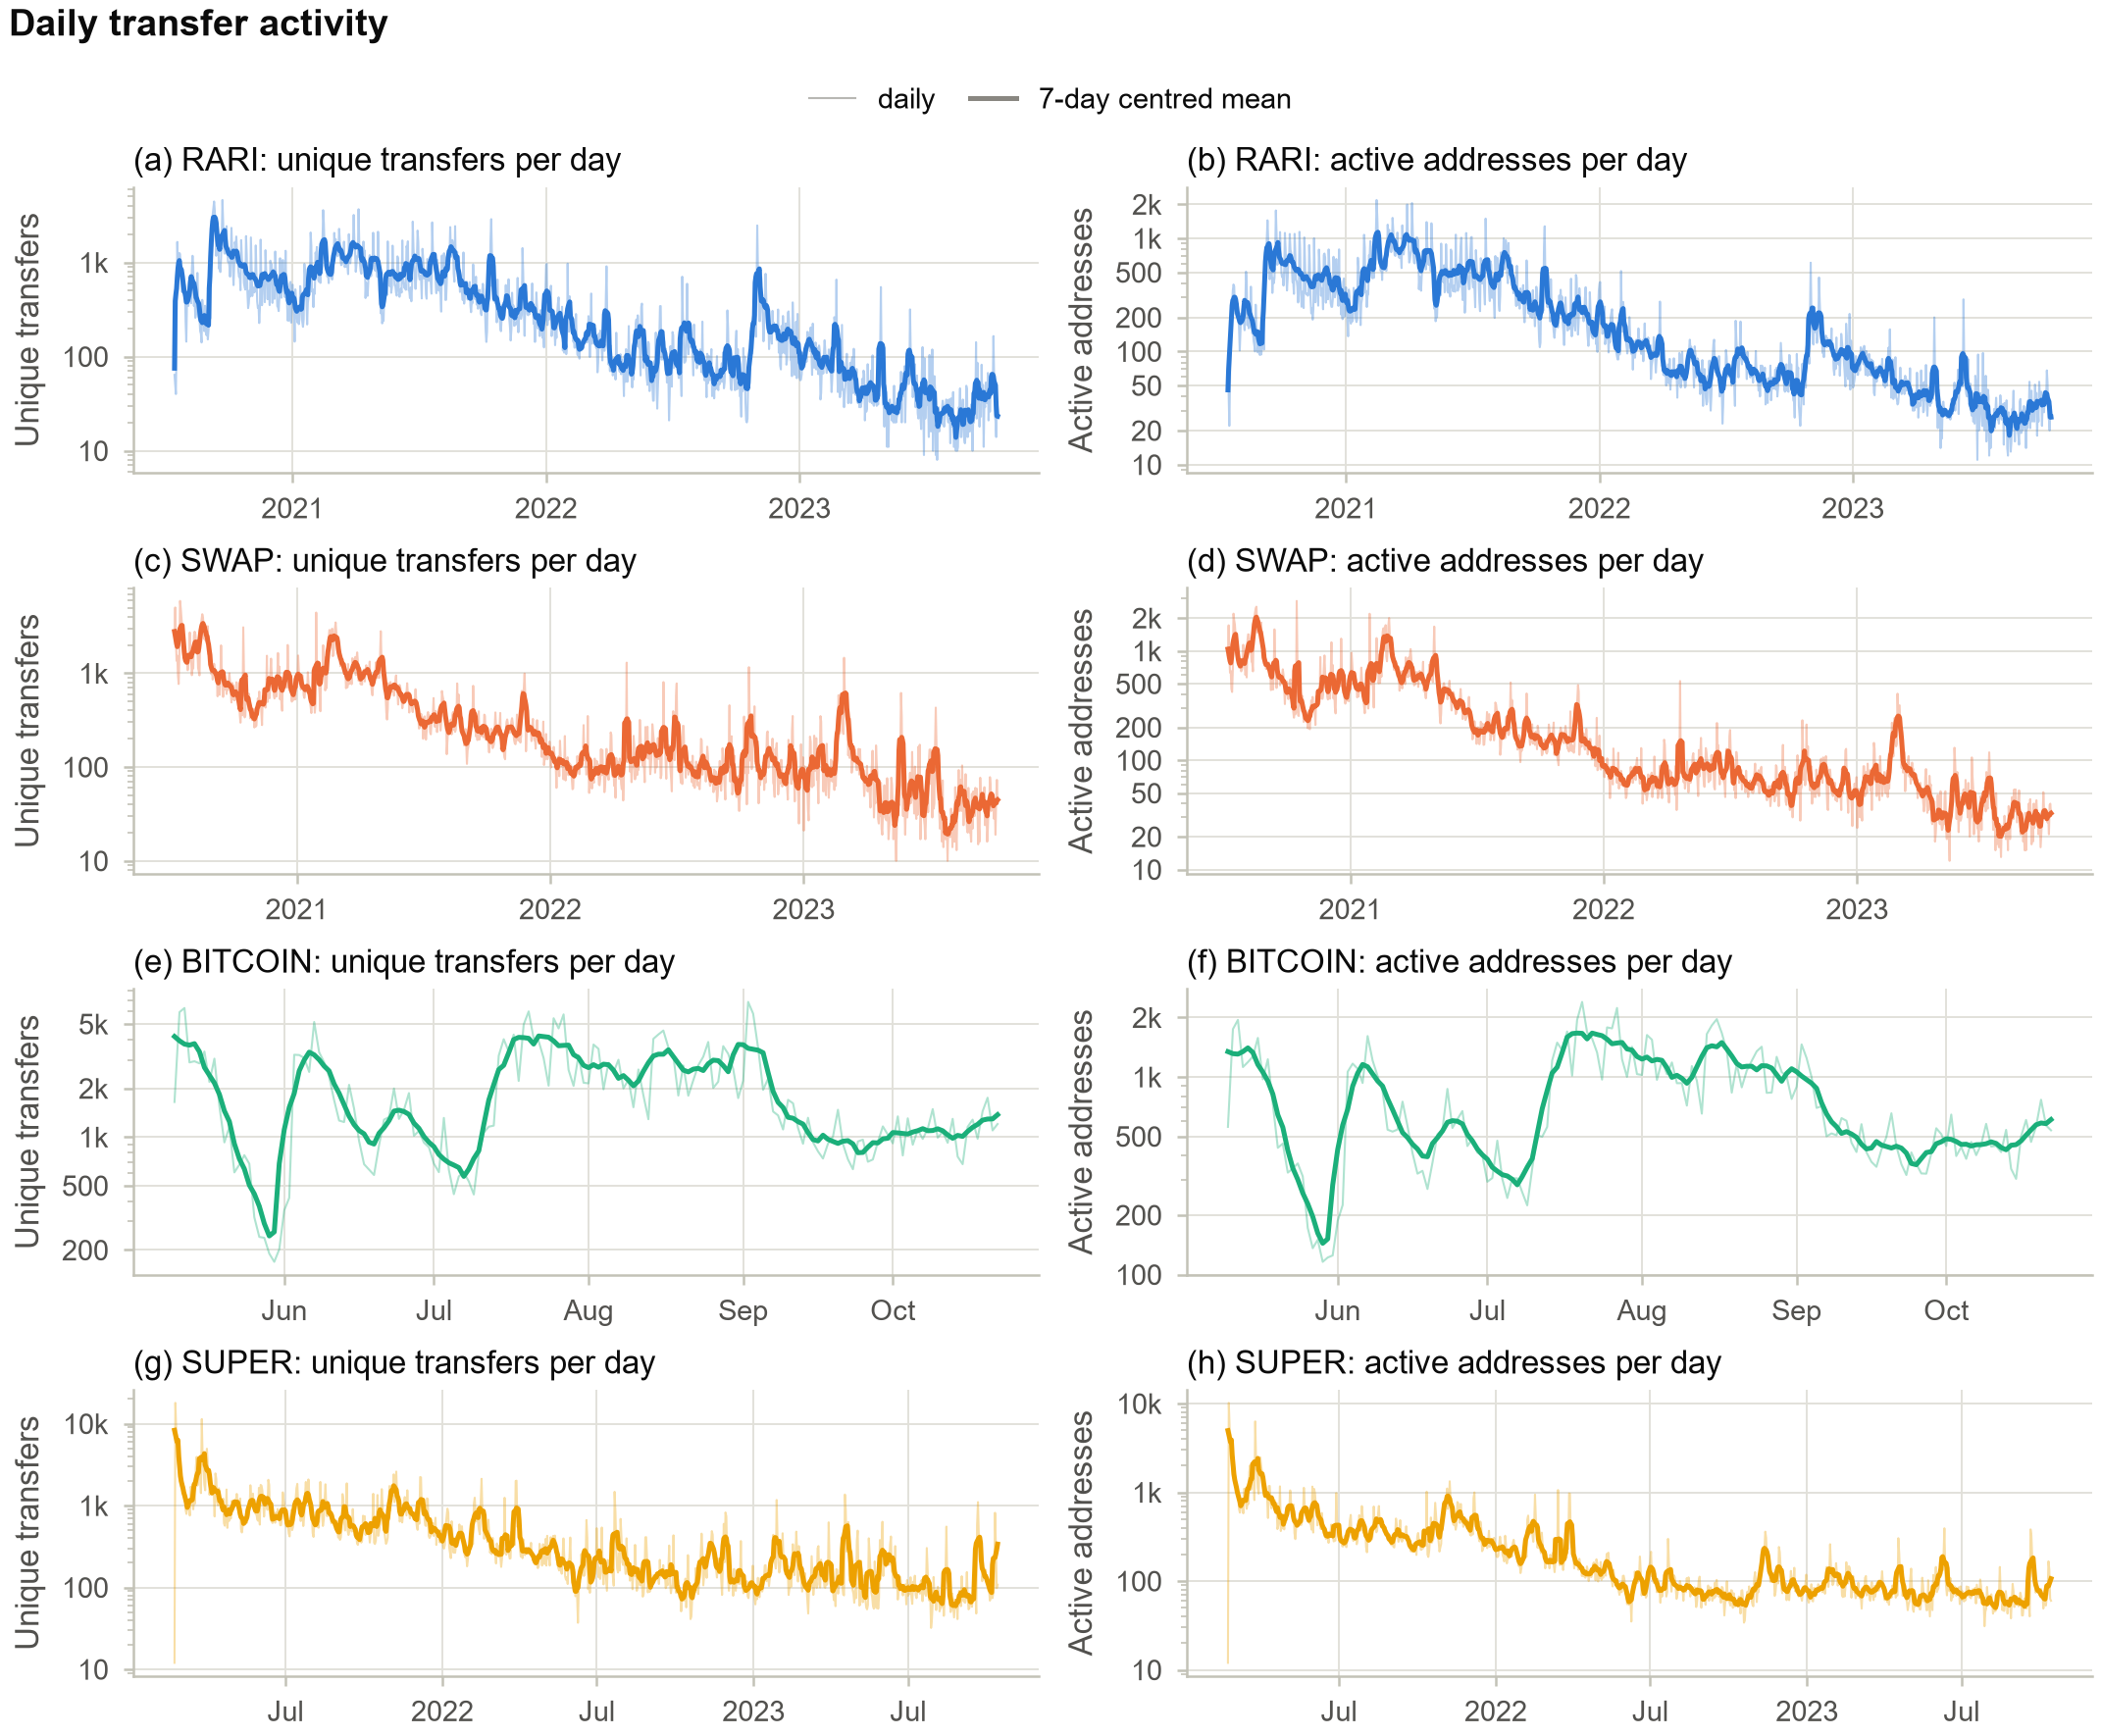
\includegraphics[width=\linewidth]{../../reports/study_A/runs/SNA/figures/fig01_daily_activity}
    \caption{Attività giornaliera per token: trasferimenti unici (sinistra) e
    indirizzi attivi (destra), in scala logaritmica. Linea sottile: valore
    giornaliero; linea spessa: media mobile centrata a 7 giorni.}
    \label{fig:fig01_daily_activity}
\end{figure}

RARI, SWAP e SUPER coprono circa tre anni e mostrano un declino di quasi due
ordini di grandezza: da circa $10^3$ trasferimenti al giorno nel 2020--2021 a
poche decine nel 2023, interrotto da picchi isolati (RARI a fine 2022, SWAP a
inizio 2023). SUPER parte da un picco iniziale vicino a $10^4$ e si assesta
attorno a $10^2$. BITCOIN copre solo cinque mesi del 2023, con un livello di
attività più alto (circa $10^3$ trasferimenti al giorno) e oscillazioni ampie,
fino a un minimo di circa 200 a fine maggio. Trasferimenti e indirizzi attivi
seguono lo stesso andamento: le variazioni dipendono da quanti indirizzi
partecipano, non da quanto è attivo ciascuno. Le \textbf{reti non} sono quindi
\textbf{stazionarie}. Un grafo aggregato sull'intero periodo mescola fasi molto diverse,
e questo giustifica l'analisi per mesi.

\subsection{Degree Distribution}
Tutte le distribuzioni si estendono su quattro o cinque ordini di grandezza.
\begin{figure}[H]
    \centering
    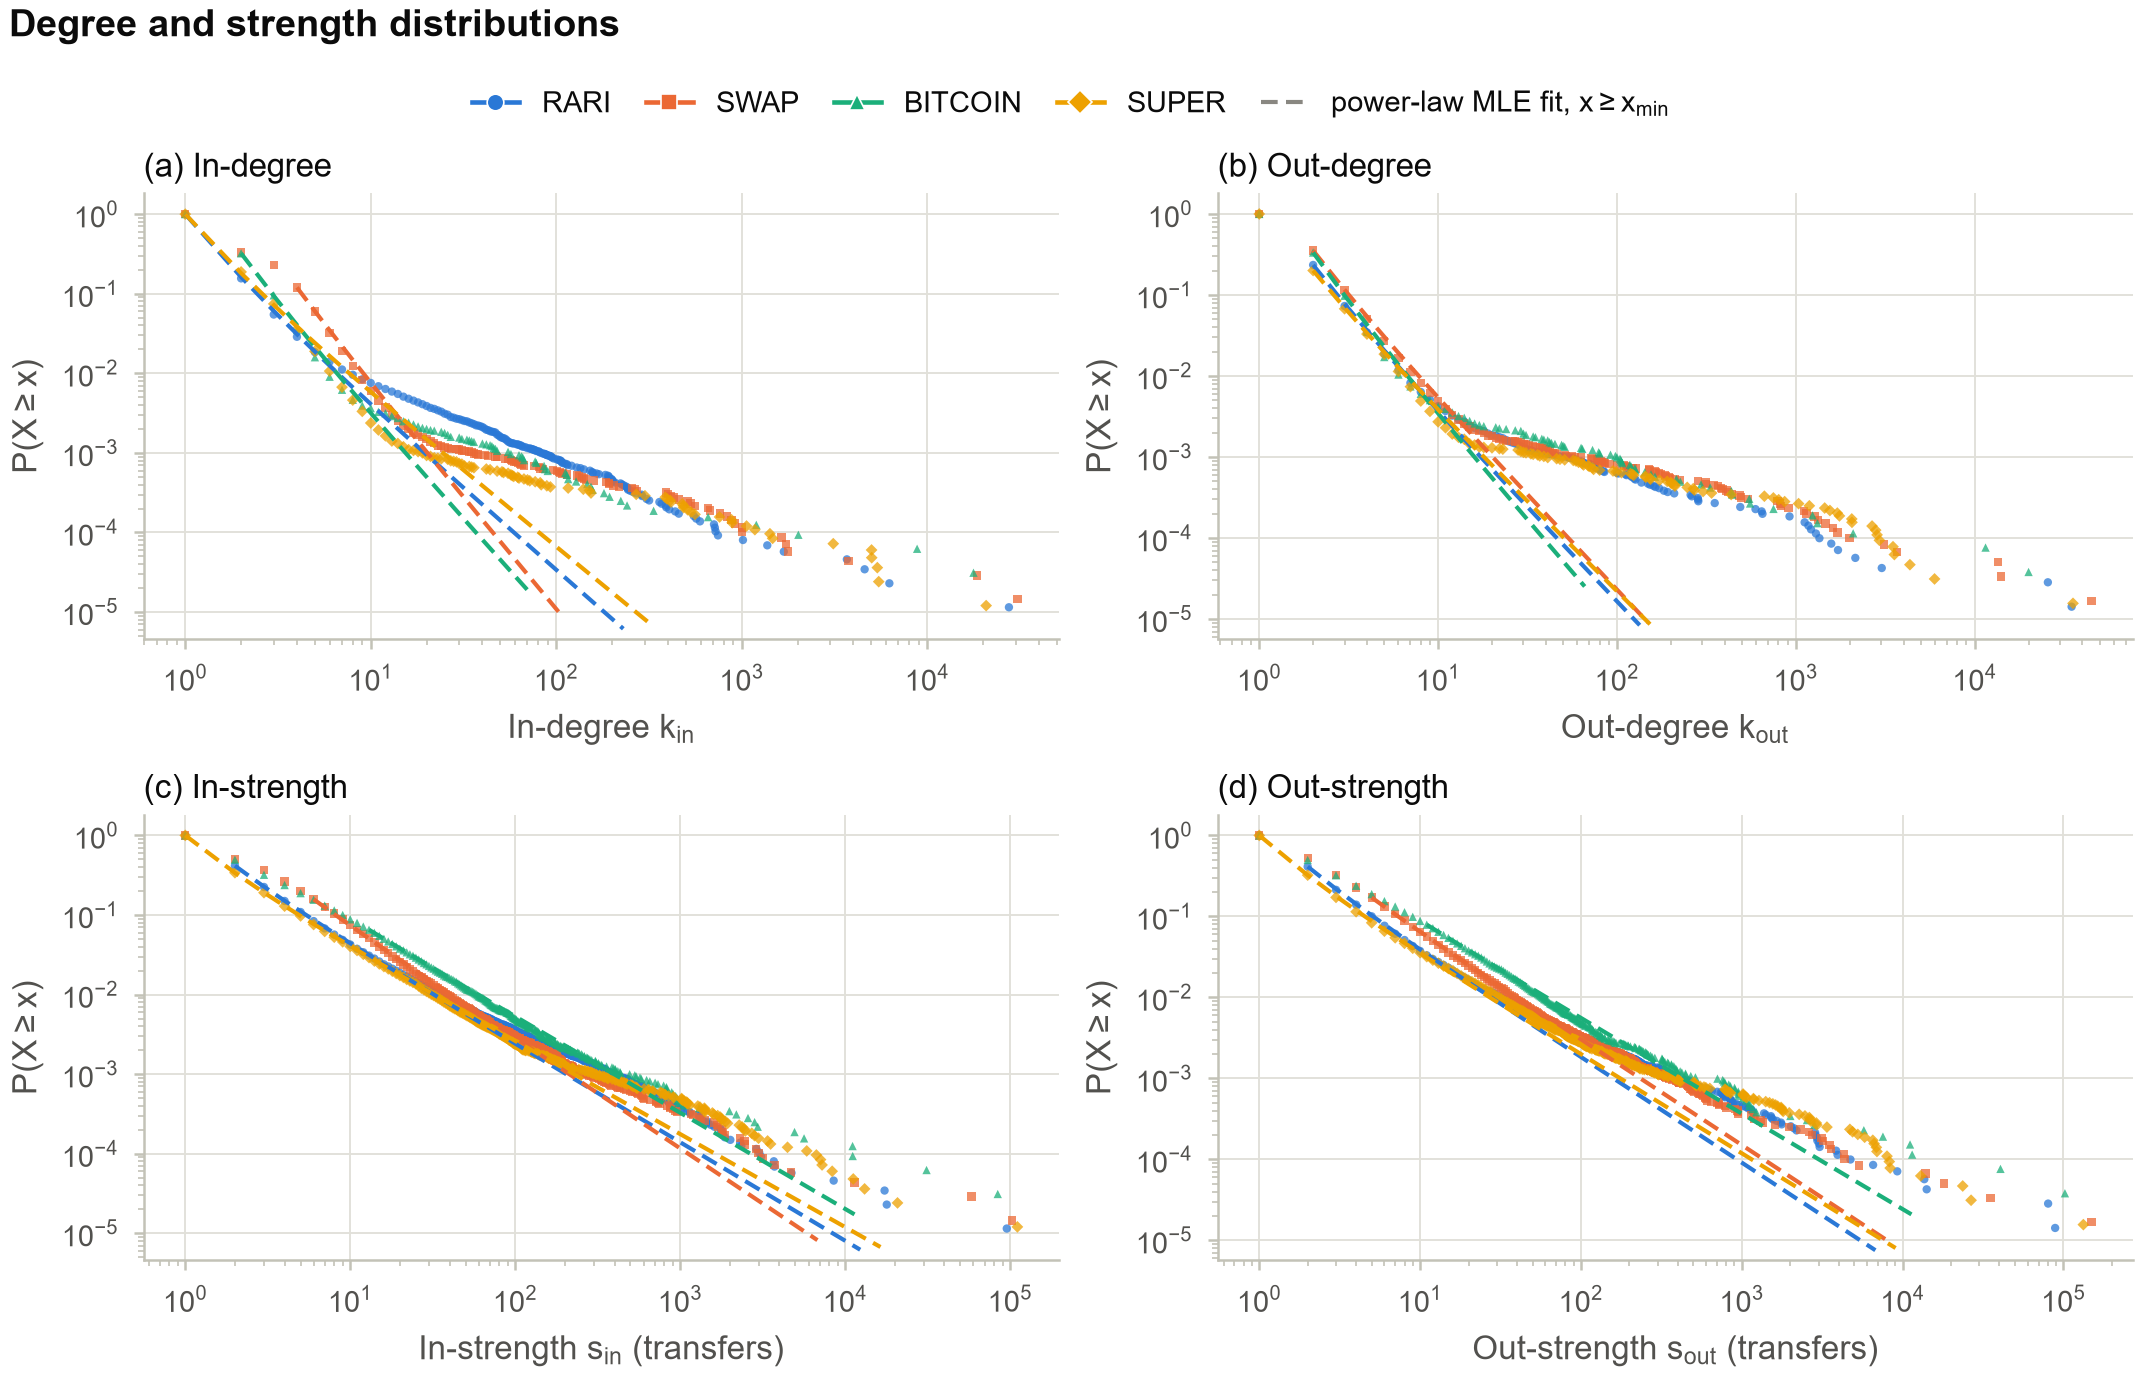
\includegraphics[width=\linewidth]{../../reports/study_A/runs/SNA/figures/fig03_degree_strength_ccdf}
    \caption{Distribuzioni complementari cumulate (CCDF) di grado e forza in
    entrata e in uscita (forza = numero di trasferimenti), sull'intero
    periodo, in scala log-log.}
    \label{fig:fig03_degree_strength_ccdf}
\end{figure}


La grande maggioranza degli indirizzi ha grado 1 o 2, mentre pochi superano
$10^4$ controparti (in-degree massimo tra $17\,778$ e $30\,657$, out-degree
massimo tra $20\,014$ e $44\,934$). Le CCDF dei gradi non sono rettilinee:
scendono ripidamente fino a circa 10 e proseguono poi con una lunga coda quasi
piatta fino a $10^3$--$10^4$, che la legge di potenza stimata non segue. 
Il numero di trasferimenti sono visivamente più vicine a una retta. Il test formale, però, rifiuta
la power-law ($p_{\mathrm{GOF}} < 0{,}1$) in 20 casi su 28 tra grado,
forza e volume \cite{clauset2009powerlaw}, e la lognormale è spesso preferibile. La power-law non
è rifiutata solo in 2 delle 12 distribuzioni di grado (in-degree di RARI e
SUPER), e per RARI anche lì la lognormale descrive meglio i dati. Le reti
hanno quindi code pesanti, ma i dati non giustificano di definirle
\emph{scale-free}.

\begin{figure}[H]
    \centering
    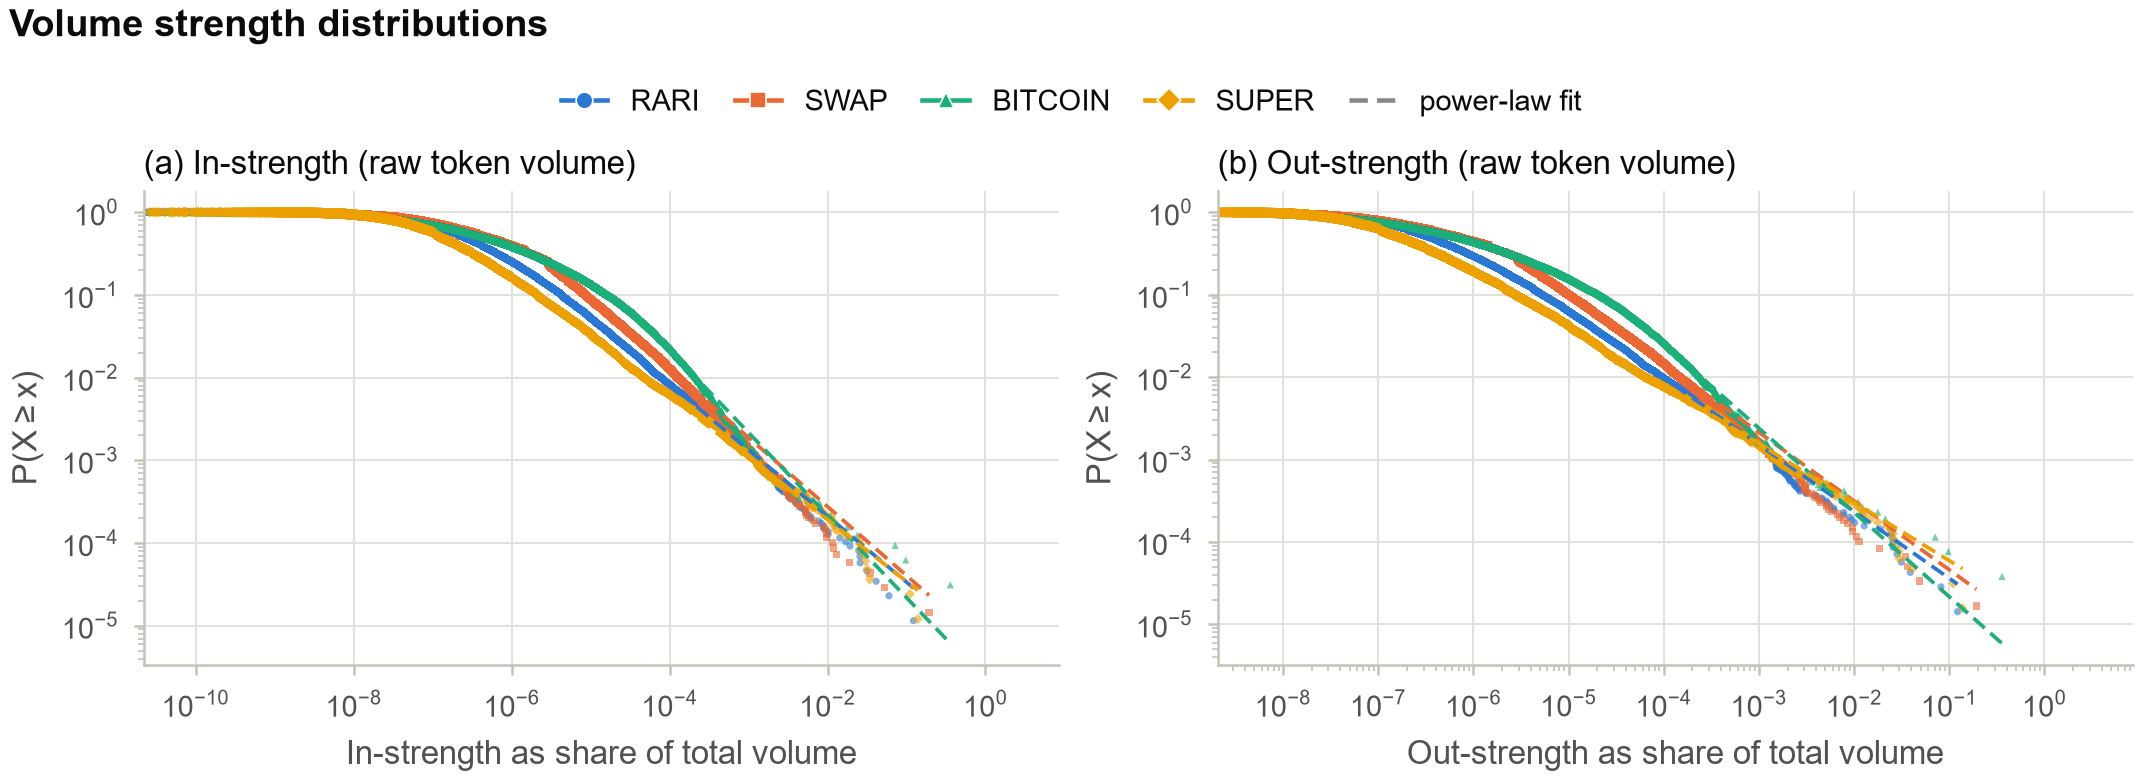
\includegraphics[width=\linewidth]{../../reports/study_A/runs/SNA/figures/fig05_volume_strength_ccdf}
    \caption{CCDF della forza in volume (importi grezzi) ricevuta e inviata,
    espressa come quota del volume totale del token per renderla
    confrontabile tra token diversi.}
    \label{fig:fig05_volume_strength_ccdf}
\end{figure}

Misurata in volume, la concentrazione è molto più estrema che nei conteggi.
La coda arriva a singoli indirizzi che ricevono o inviano dal 10\% al 40\% di
tutto il volume del token. L'indice di Gini dell'out-strength in volume va da
$0{,}95$ (SWAP) a $0{,}99$ (SUPER), e l'1\% degli indirizzi più attivi muove
tra il 76\% e il 92\% del volume. La metà del volume inviato è concentrata in
42 indirizzi per SWAP, 20 per RARI, 12 per SUPER e appena 3 per BITCOIN. Le
quattro curve si sovrappongono quasi del tutto nella coda, quindi il grado di
concentrazione è simile nonostante popolazioni e periodi diversi. 
La power-law non è rifiutata solo per RARI ($p = 0{,}10$ e $0{,}20$).

\subsection{Analisi di diverse metriche }
\begin{figure}[H]
    \centering
    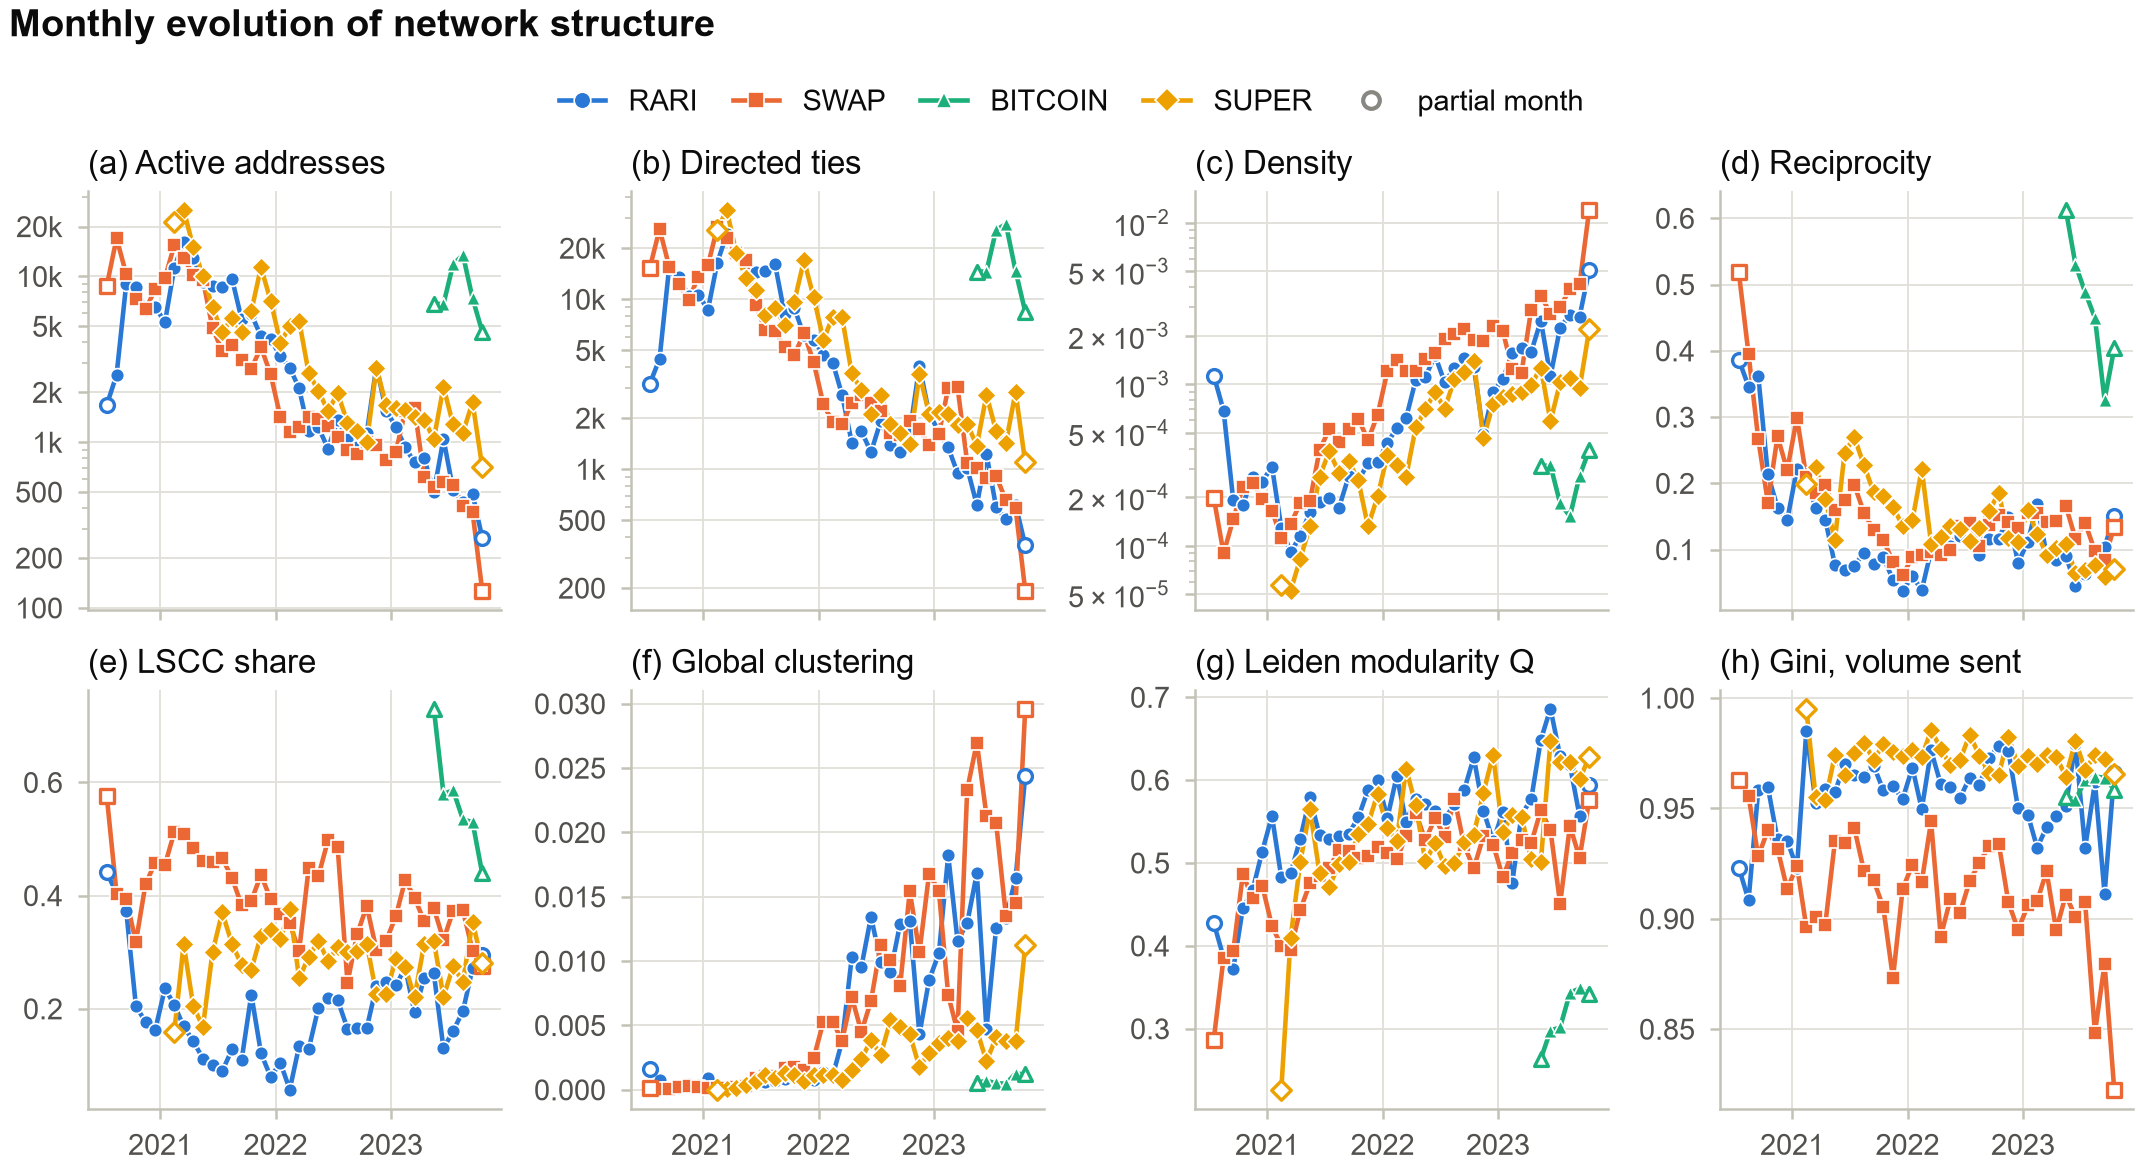
\includegraphics[width=\linewidth]{../../reports/study_A/runs/SNA/figures/fig07_temporal_structure}
    \caption{Evoluzione mensile della struttura attraverso diverse metriche. I marcatori vuoti sono mesi coperti per meno dell'80\%.}
    \label{fig:fig07_temporal_structure}
\end{figure}

Il numero di indirizzi attivi e di legami diretti cala di circa due ordini di
grandezza (a, b). Nello stesso periodo densità (c) e clustering (f) crescono:
è un effetto della dimensione, perché a grado medio costante la densità
scala come $1/n$, e non indica legami più fitti. La reciprocità (d) scende da
$0{,}4$--$0{,}5$ a circa $0{,}1$: i flussi diventano quasi solo
unidirezionali. Su base mensile la componente fortemente connessa raccoglie
solo il 5--50\% degli indirizzi (e), molto meno che sull'intero periodo. Dopo i primi
mesi la modularità (g) \cite{newman2006modularity} resta stabile tra $0{,}45$ e $0{,}65$ per RARI, SWAP e SUPER,
quindi la presenza di community non dipende dalla scala della rete. BITCOIN si
discosta su tutte le misure: reciprocità più alta ($0{,}3$--$0{,}6$),
modularità più bassa ($0{,}26$--$0{,}35$), componente forte più ampia. Il Gini
del volume inviato (h) resta sopra $0{,}85$ in tutti i mesi, e per lo più
sopra $0{,}95$: la concentrazione del volume è una caratteristica permanente,
non legata a una fase particolare.


\subsection{Confronto con Null Model}
\begin{figure}[H]
    \centering
    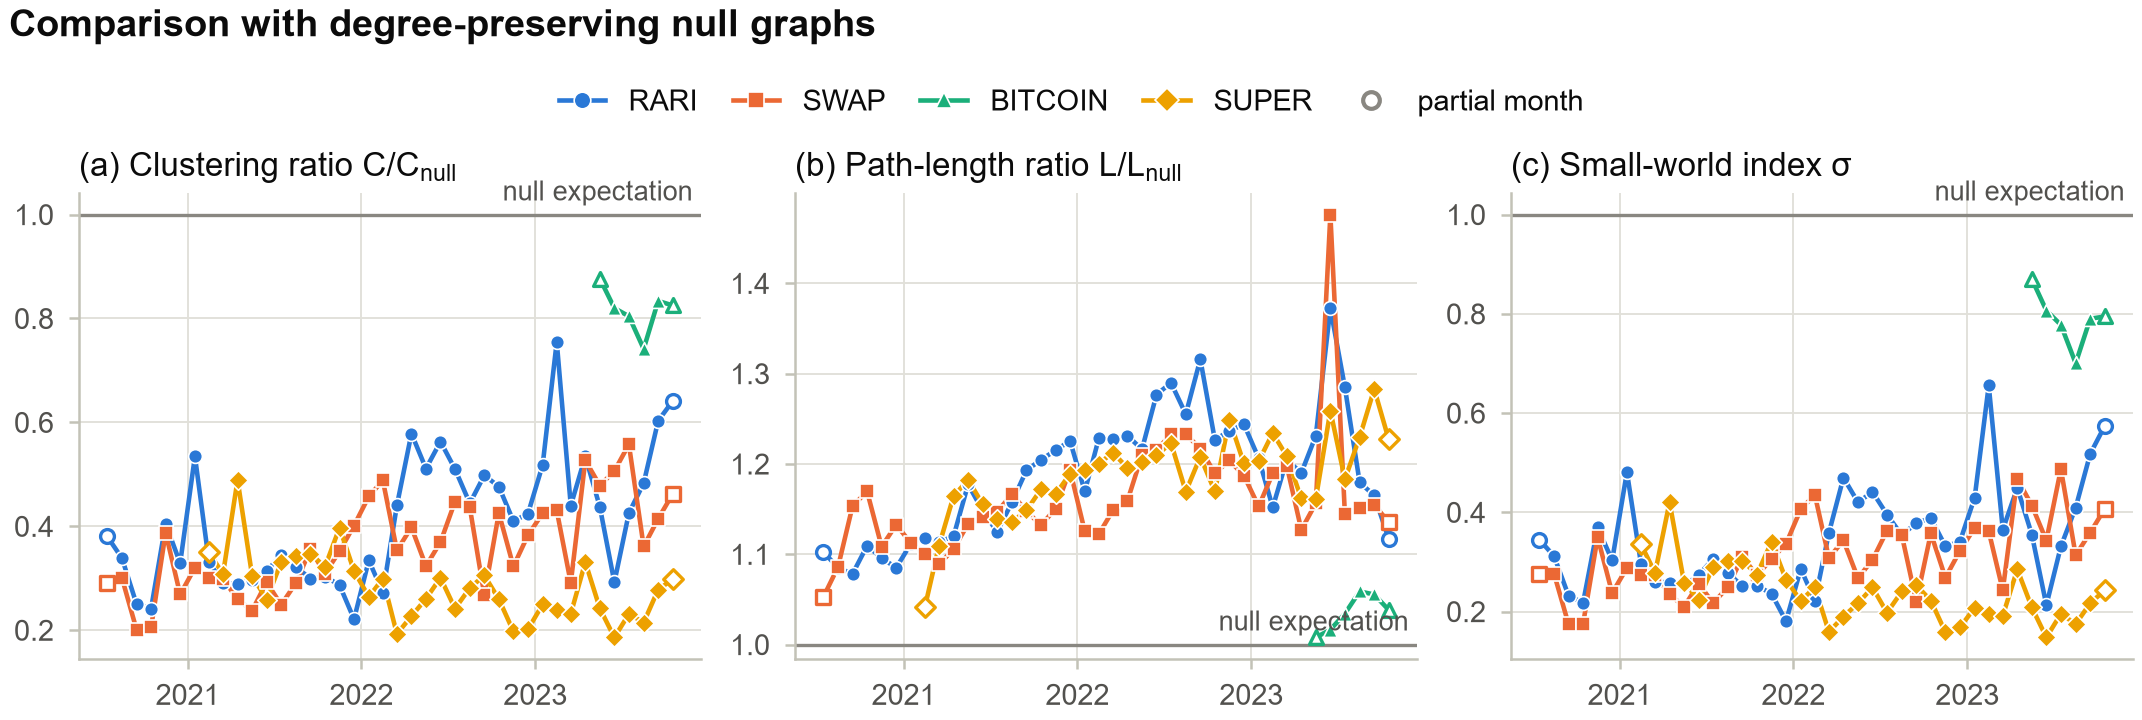
\includegraphics[width=\linewidth]{../../reports/study_A/runs/SNA/figures/fig08_small_world}
    \caption{Confronto mensile con 15 grafi nulli che preservano la sequenza
    dei gradi: rapporto di clustering $C/C_{\mathrm{null}}$ (a), rapporto
    di lunghezza media dei cammini $L/L_{\mathrm{null}}$ (b) e indice
    small-world $\sigma$ (c), sulla proiezione non diretta.}
    \label{fig:fig08_small_world}
\end{figure}

Una rete si considera \textbf{
small-world} quando ha molto \textbf{più clustering del modello nullo} ($C/C_{\mathrm{null}} \gg 1$) e cammini di lunghezza comparabile
($L/L_{\mathrm{null}} \approx 1$) \cite{watts1998smallworld}, cioè
$\sigma = (C/C_{\mathrm{null}})/(L/L_{\mathrm{null}}) > 1$
\cite{humphries2008smallworldness}. In ogni mese e per ogni token accade il
contrario. Il clustering è \emph{inferiore} a quello atteso
($0{,}2$--$0{,}75$ per i token maggiori, $0{,}75$--$0{,}87$ per BITCOIN), i
cammini sono fino al 47\% più lunghi del nullo, e quindi $\sigma$ resta
sempre sotto 1. Sull'intero periodo $\sigma$ va da $0{,}32$ (SUPER) a
$0{,}72$ (BITCOIN). Le distanze medie sono comunque brevi (da $2{,}4$ a
$3{,}2$ passi), ma lo sono già nel modello nullo: si spiegano con la sequenza
dei gradi, non con un'organizzazione small-world. Il deficit di triangoli è
coerente con la forte disassortatività di grado \cite{newman2002assortative} (da $-0{,}25$ a $-0{,}48$). Gli \textbf{
hub} sono \textbf{collegati} soprattutto a indirizzi periferici che non comunicano tra
loro, \textbf{come} in una \textbf{struttura a stella} (\emph{hub-and-spoke}).\\
Vanno però lette come vicinanza nella rete delle interazioni,
indipendentemente dal verso dei trasferimenti, e non come percorsi effettivamente seguibili da un flusso di token.\\
Nel grafo orientato solo gli indirizzi del nucleo fortemente connesso (47--84\% sull'intero periodo, Figura~\ref{fig:fig10_bowtie})
si raggiungono reciprocamente, e per molte coppie non esiste alcun cammino diretto.
Il \textbf{rifiuto} dell'\textbf{ipotesi small-world} è evidente: la proiezione aggiunge cammini e quindi favorisce $\sigma > 1$ e dunque stiamo anche sovrastimando il vero valore.
Mentre il vero valore di $\sigma$ è determinato soprattutto dal deficit di triangoli,
che la proiezione può solo sovrastimare rispetto al grafo diretto.\\
In generale ci si aspettava tale esito poiché si tratta di un grafo reale che rappresenta un comportamento come definito Hub-centric. 

\subsection{Struttura Bow-tie del grafo}
Sfruttiamo la decomposizione bow-tie \cite{broder2000bowtie} per dividere gli indirizzi in:
\begin{figure}[H]
    \centering
    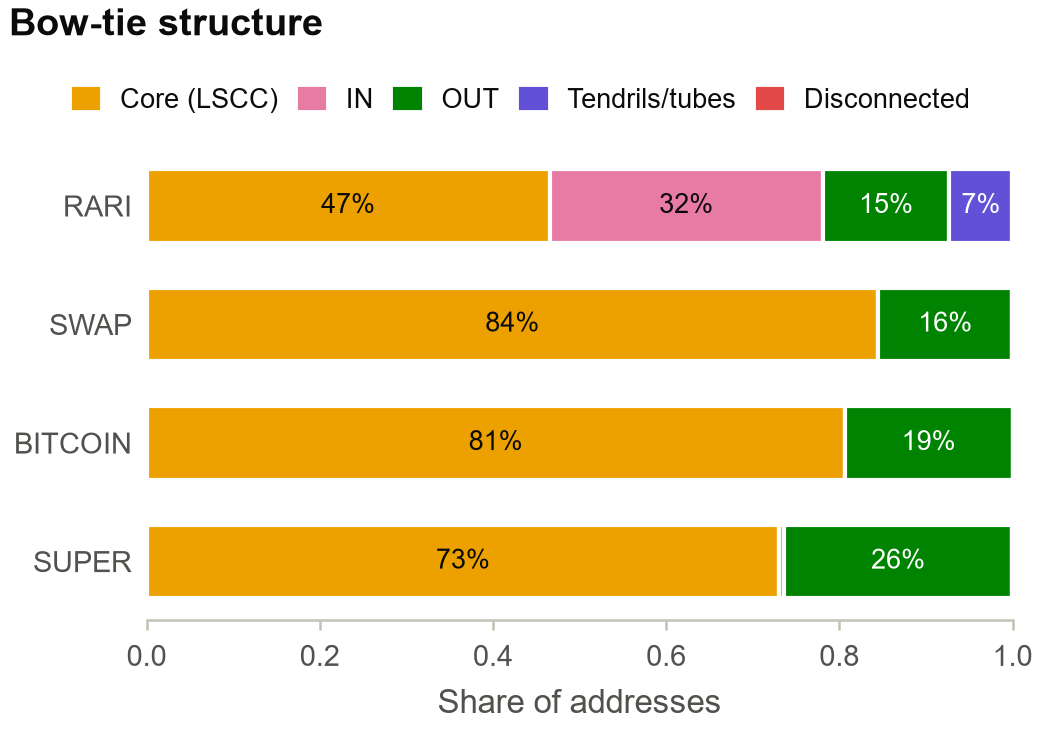
\includegraphics[width=0.65\linewidth]{../../reports/study_A/runs/SNA/figures/fig10_bowtie}
    \caption{Decomposizione bow-tie del grafo diretto sull'intero periodo
    attorno alla componente fortemente connessa più grande (\emph{core}).}
    \label{fig:fig10_bowtie}
\end{figure}

nucleo, IN (indirizzi che raggiungono il nucleo senza esserne raggiunti), OUT
(raggiunti dal nucleo senza raggiungerlo), tendrils/tubes (collegati a IN o
OUT ma non al nucleo) e componenti scollegate.
In SWAP, BITCOIN e SUPER il grafo si divide quasi interamente in due parti:
un nucleo fortemente connesso (73--84\% degli indirizzi) e un insieme OUT
(16--26\%) di indirizzi raggiunti dal nucleo da cui non riparte alcun flusso
verso di esso. L'insieme OUT corrisponde in larga parte agli indirizzi che si
limitano a ricevere (dal 14\% al 23\% del totale). L'insieme \textbf{IN è assente},
\textbf{coerentemente} con il fatto che per inviare un token bisogna \textbf{prima} averlo
\textbf{ricevuto}. RARI ha un nucleo molto più piccolo (47\%) e una struttura più
articolata: il 32\% degli indirizzi appartiene a IN, cioè invia verso il
nucleo senza esserne raggiungibile, e il 7\% sta in tendrils/tubes. In RARI,
quindi, una parte rilevante dei flussi entra nel nucleo da una periferia che
il nucleo stesso non alimenta.
Dunque una caratteristica particolare, che invoglia ovviamente ad analizzare la struttura in se del Token.
Così da capire chi sono gli indirizzi che generano questi flussi entranti di moneta.


\subsection{Grafo statico o in evoluzione?}
Come ci si aspetta da una rete che analizza transizioni block-chain, il ricambio è molto alto.
\begin{figure}[H]
    \centering
    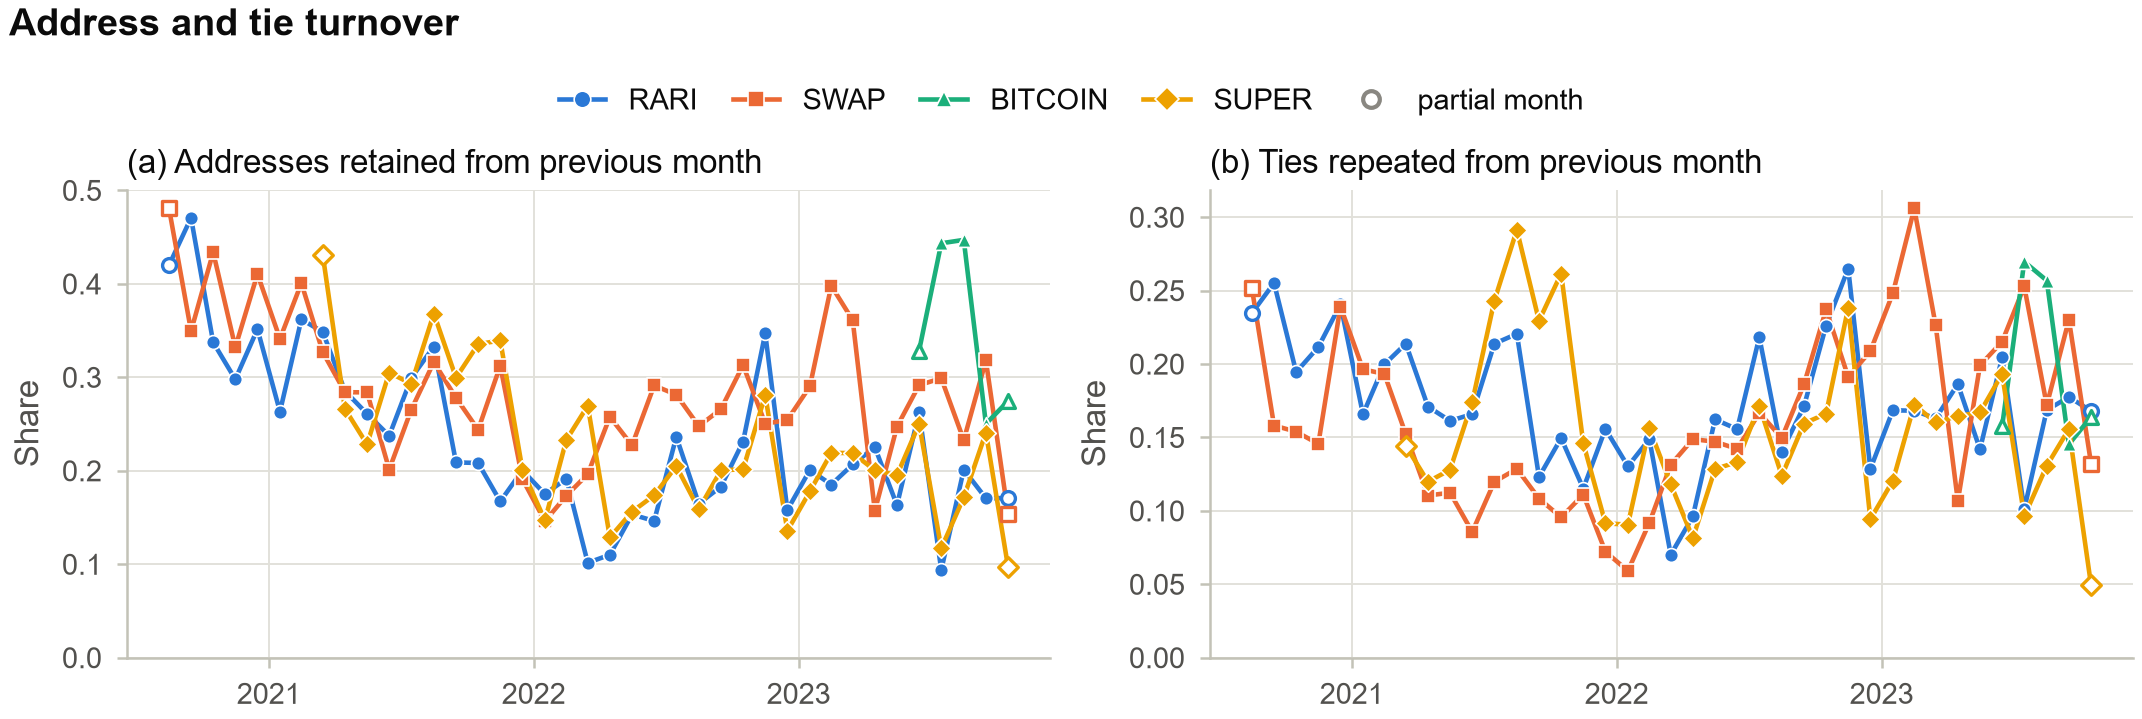
\includegraphics[width=\linewidth]{../../reports/study_A/runs/SNA/figures/fig13_turnover}
    \caption{Ricambio mensile: quota degli indirizzi attivi nel mese
    precedente che sono di nuovo attivi (a) e quota dei legami diretti del
    mese precedente che si ripetono (b).}
    \label{fig:fig13_turnover}
\end{figure}

Da un mese al successivo resta attivo solo il
10--48\% degli indirizzi, con un calo da circa il 40\% nel 2020 al 10--30\%
nel 2023, e si ripete solo il 5--30\% dei legami diretti. La maggior parte
dell'attività di ogni mese coinvolge quindi indirizzi o coppie nuovi rispetto
al mese precedente. Questo ha due conseguenze. Le misure calcolate su un mese
descrivono una popolazione in larga parte diversa da quella del mese prima.
La piccola quota di indirizzi e legami persistenti suggerisce l'esistenza di un nucleo stabile di partecipanti ricorrenti.
Questo \textbf{nucleo} è compatibile con \textbf{entità ad attività continuativa}, come \textbf{contratti} di protocollo, \textbf{exchange} o trader automatizzati o non.
Senza etichette esterne, però, non è possibile attribuire questi indirizzi a una specifica tipologia di entità reale.

\subsection{Community Detection}
Attraverso Leiden sono state identificate diverse community\cite{traag2019leiden} (risoluzione 1, seed fisso) sulla proiezione non diretta del grafo dei trasferimenti.
% Griglia 2x2 dei grafi quoziente delle community
\begin{figure}[H]
    \centering
    \begin{subfigure}[b]{0.49\linewidth}
        \centering
        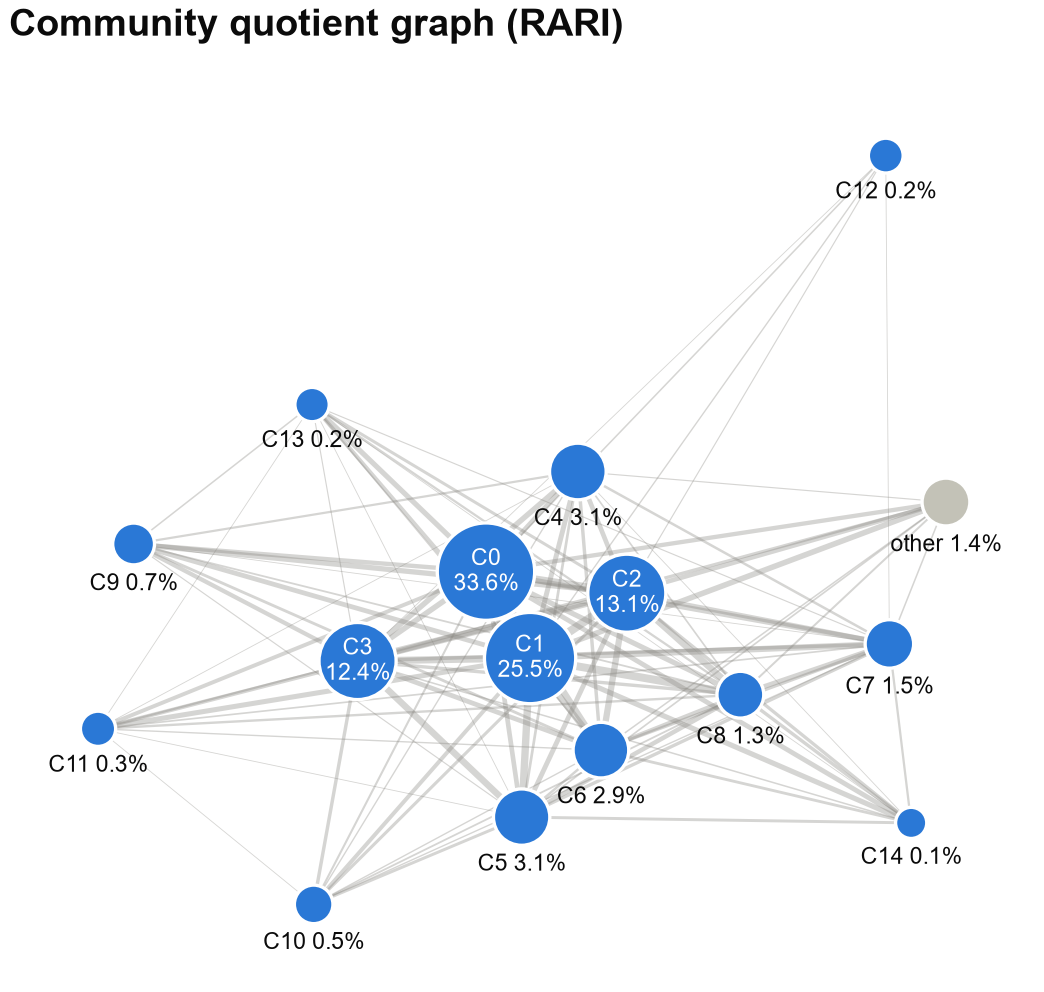
\includegraphics[width=\linewidth]{../../reports/study_A/runs/SNA/figures/fig16_1_community_quotient_RARI}
        \label{fig:fig16_1_community_quotient_rari}
    \end{subfigure}\hfill
    \begin{subfigure}[b]{0.49\linewidth}
        \centering
        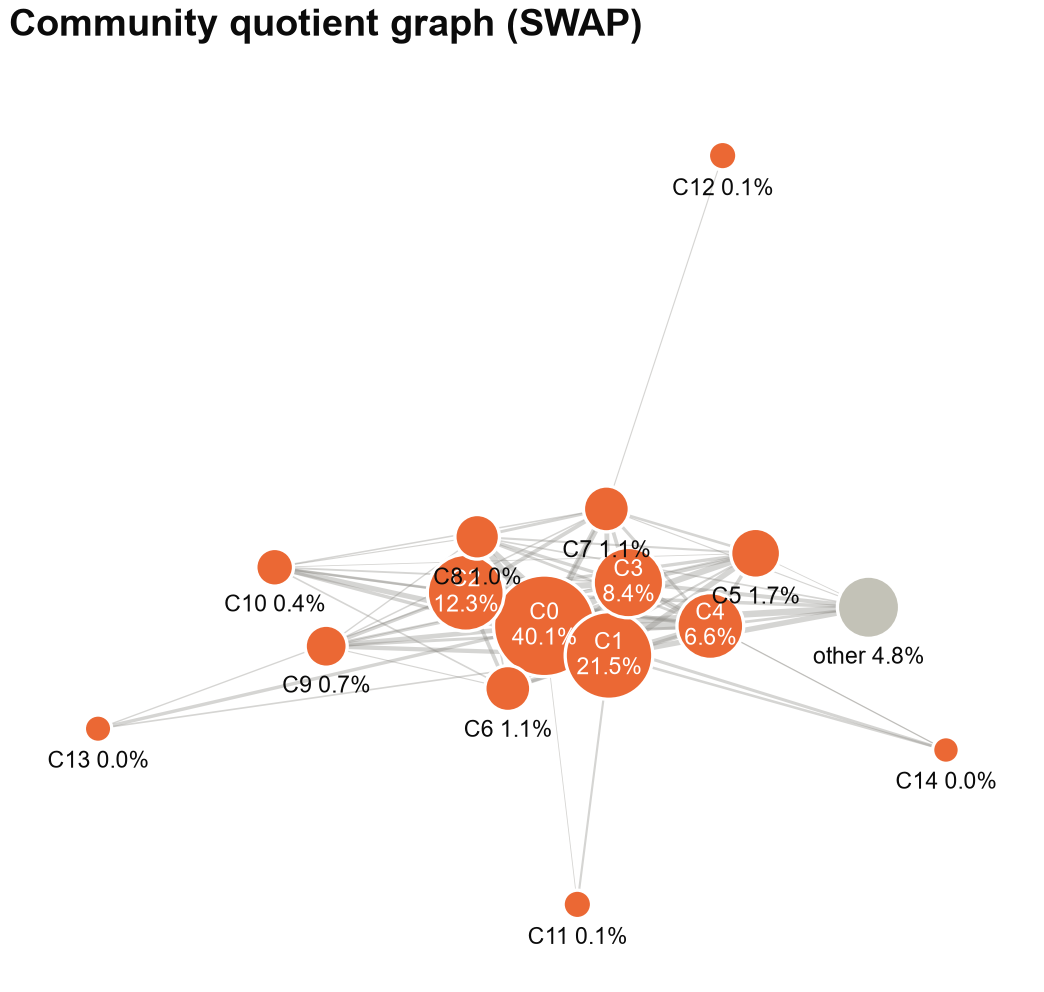
\includegraphics[width=\linewidth]{../../reports/study_A/runs/SNA/figures/fig16_2_community_quotient_SWAP}
        \label{fig:fig16_2_community_quotient_swap}
    \end{subfigure}

    \vspace{0.5em}
    \begin{subfigure}[b]{0.49\linewidth}
        \centering
        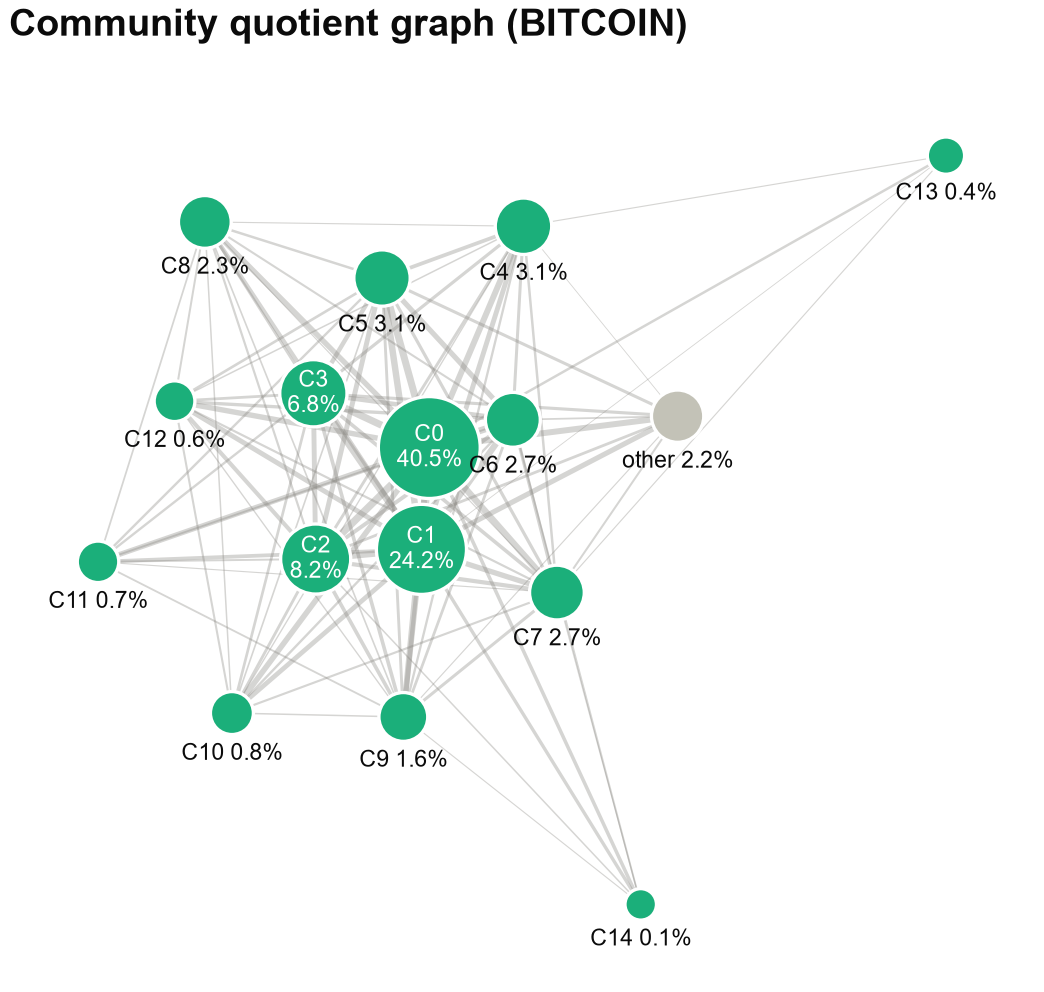
\includegraphics[width=\linewidth]{../../reports/study_A/runs/SNA/figures/fig16_3_community_quotient_BITCOIN}
        \label{fig:fig16_3_community_quotient_bitcoin}
    \end{subfigure}\hfill
    \begin{subfigure}[b]{0.49\linewidth}
        \centering
        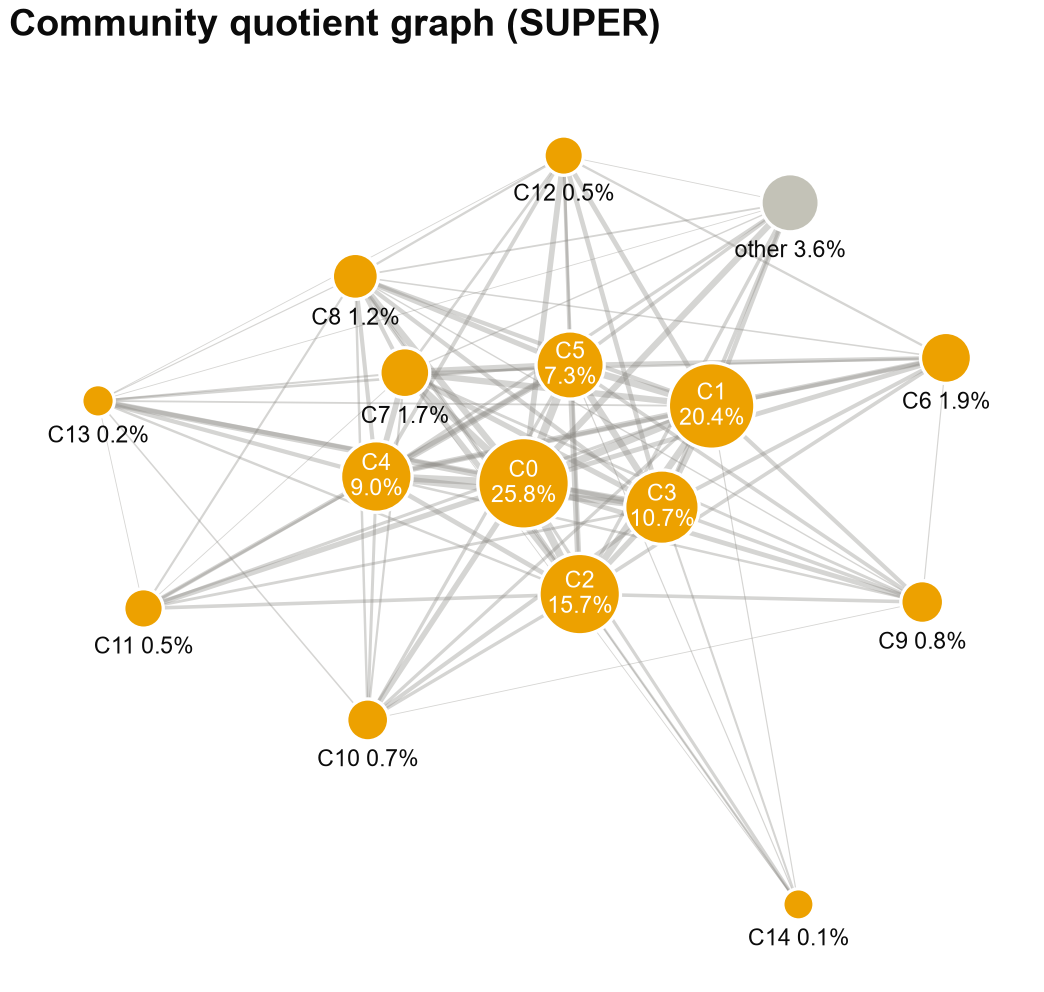
\includegraphics[width=\linewidth]{../../reports/study_A/runs/SNA/figures/fig16_4_community_quotient_SUPER}
        \label{fig:fig16_4_community_quotient_super}
    \end{subfigure}
    \caption{Grafi quoziente delle community Leiden sull'intero periodo. Ogni nodo è una delle 15
    community più grandi (area e etichetta = quota di indirizzi), le restanti
    sono riunite in \emph{other}. Lo spessore degli archi è proporzionale a
    $\log(1 + \text{trasferimenti tra community})$. La disposizione è
    arbitraria: le distanze non hanno significato.}
    \label{fig:fig16_community_quotient}
\end{figure}

Il peso di ogni coppia è il numero totale di trasferimenti nei due versi.
La direzione dei flussi quindi non entra nella partizione.
In tutti i token poche community grandi raccolgono la maggior parte degli
indirizzi. La community maggiore ne contiene dal 26\% (SUPER) al 41\% (SWAP,
BITCOIN), e le prime dieci ne coprono il 94--97\%, a fronte di un numero
totale di community che va da 251 (BITCOIN) a $1\,371$ (SWAP). Si tratta per
lo più di gruppi minuscoli (mediana di 2--3 indirizzi). Le community
principali sono però collegate tutte con tutte da archi spessi: la \textbf{rete} non è
divisa in blocchi isolati, ma è un insieme di \textbf{gruppi densi} con molti \textbf{scambi
tra loro}. Lo confermano modularità intermedie, da $0{,}30$ (BITCOIN) a
$0{,}52$ (RARI). BITCOIN ha la struttura meno separata, come già indicato
dalla sua modularità mensile più bassa (Figura~\ref{fig:fig07_temporal_structure}g).
Ovviamente le community sono raggruppamenti di indirizzi che si scambiano
molti trasferimenti, non gruppi di utenti del mondo reale.

\subsection{Community e PageRank}
I campioni rendono visibile la \textbf{struttura a stella} individuata dalle misure
aggregate.
% Griglia 2x2 dei campioni di rete
\begin{figure}[H]
    \centering
    \begin{subfigure}[b]{0.49\linewidth}
        \centering
        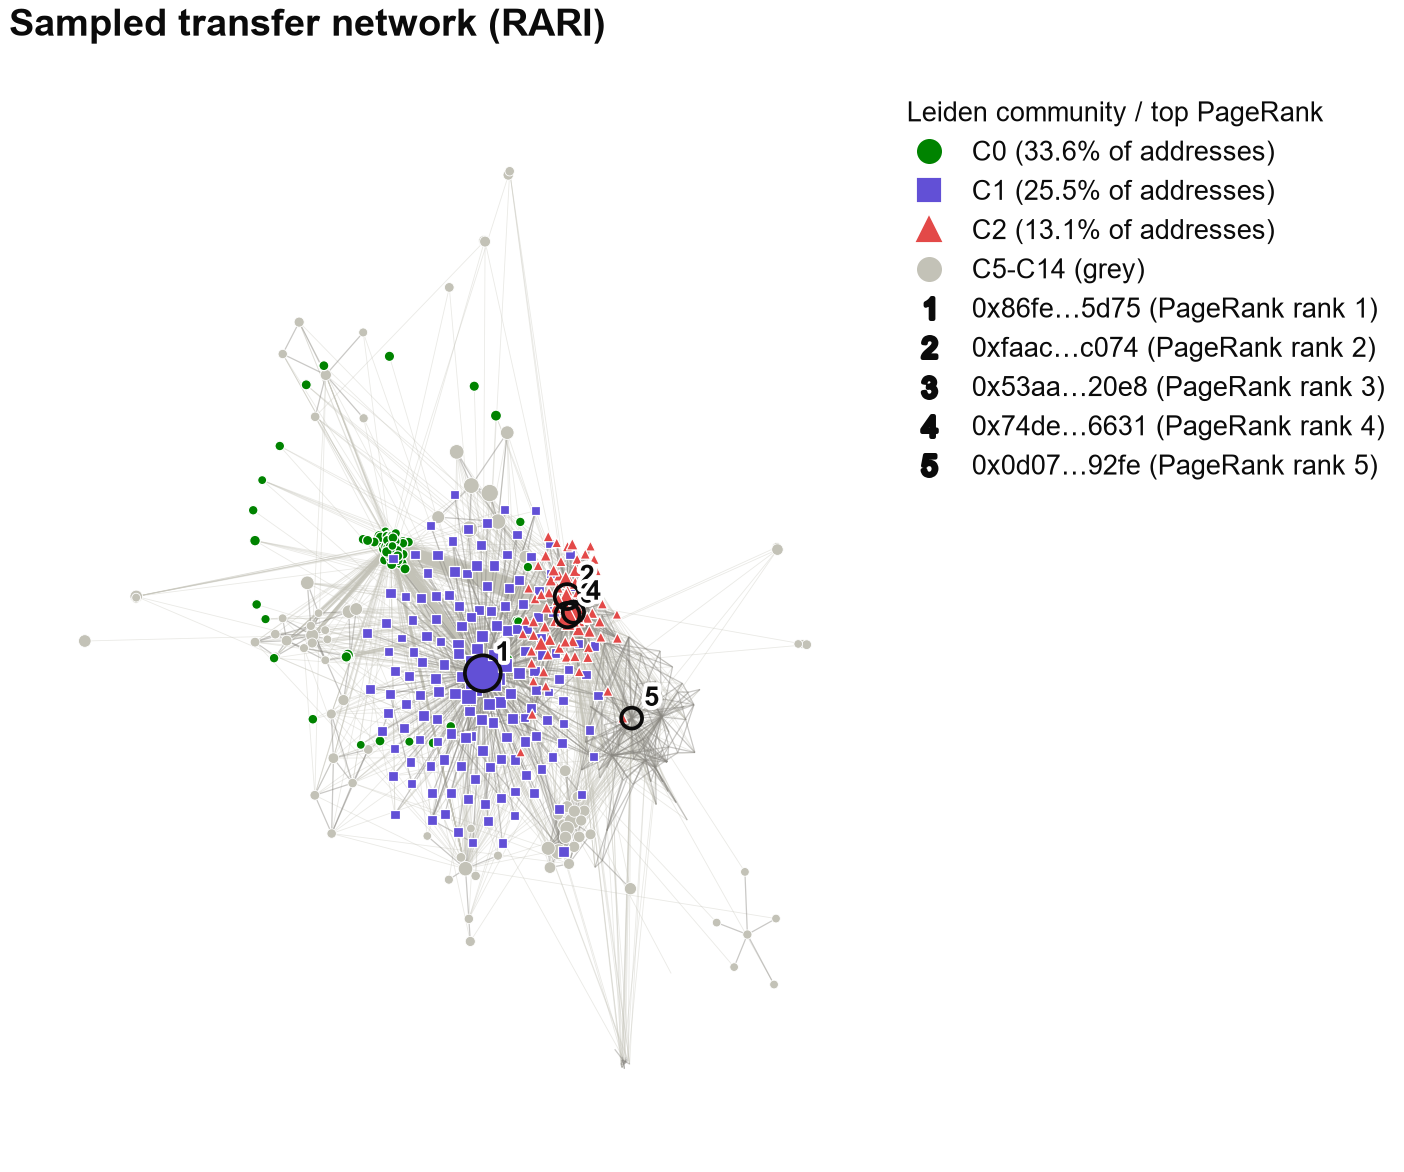
\includegraphics[width=\linewidth]{../../reports/study_A/runs/SNA/figures/fig17_1_network_sample_RARI}
        \caption{RARI ($616$ di $87\,031$ indirizzi)}
        \label{fig:fig17_1_network_sample_rari}
    \end{subfigure}\hfill
    \begin{subfigure}[b]{0.49\linewidth}
        \centering
        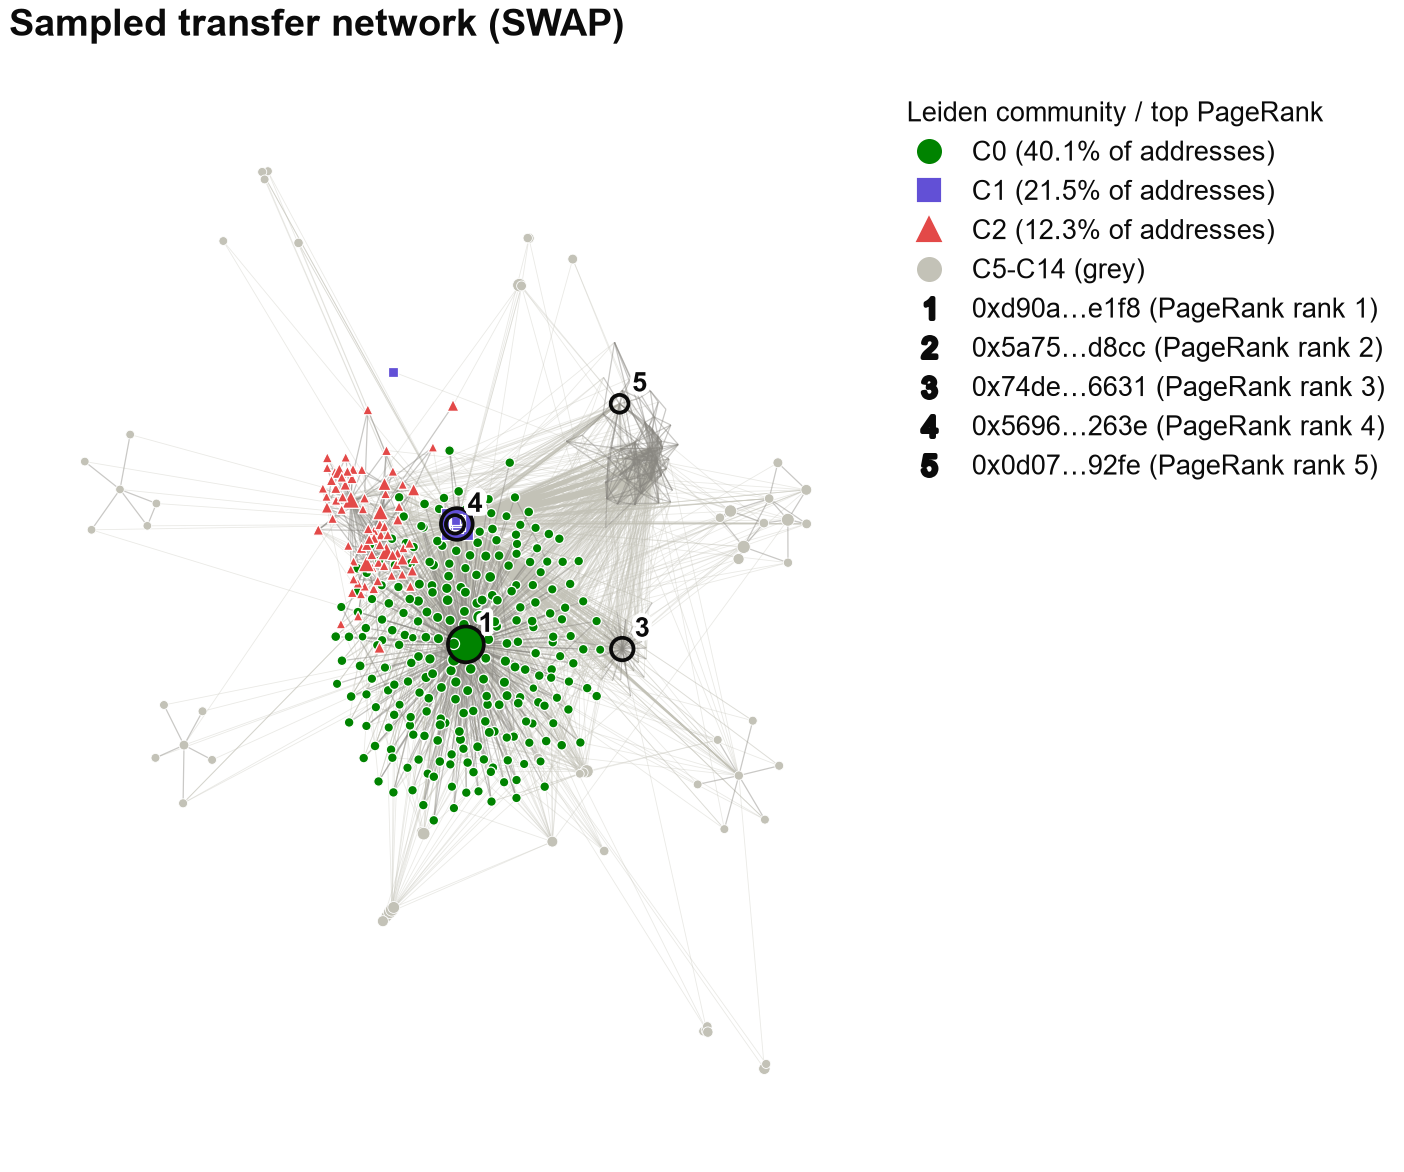
\includegraphics[width=\linewidth]{../../reports/study_A/runs/SNA/figures/fig17_2_network_sample_SWAP}
        \caption{SWAP ($619$ di $69\,121$ indirizzi)}
        \label{fig:fig17_2_network_sample_swap}
    \end{subfigure}

    \vspace{0.5em}
    \begin{subfigure}[b]{0.49\linewidth}
        \centering
        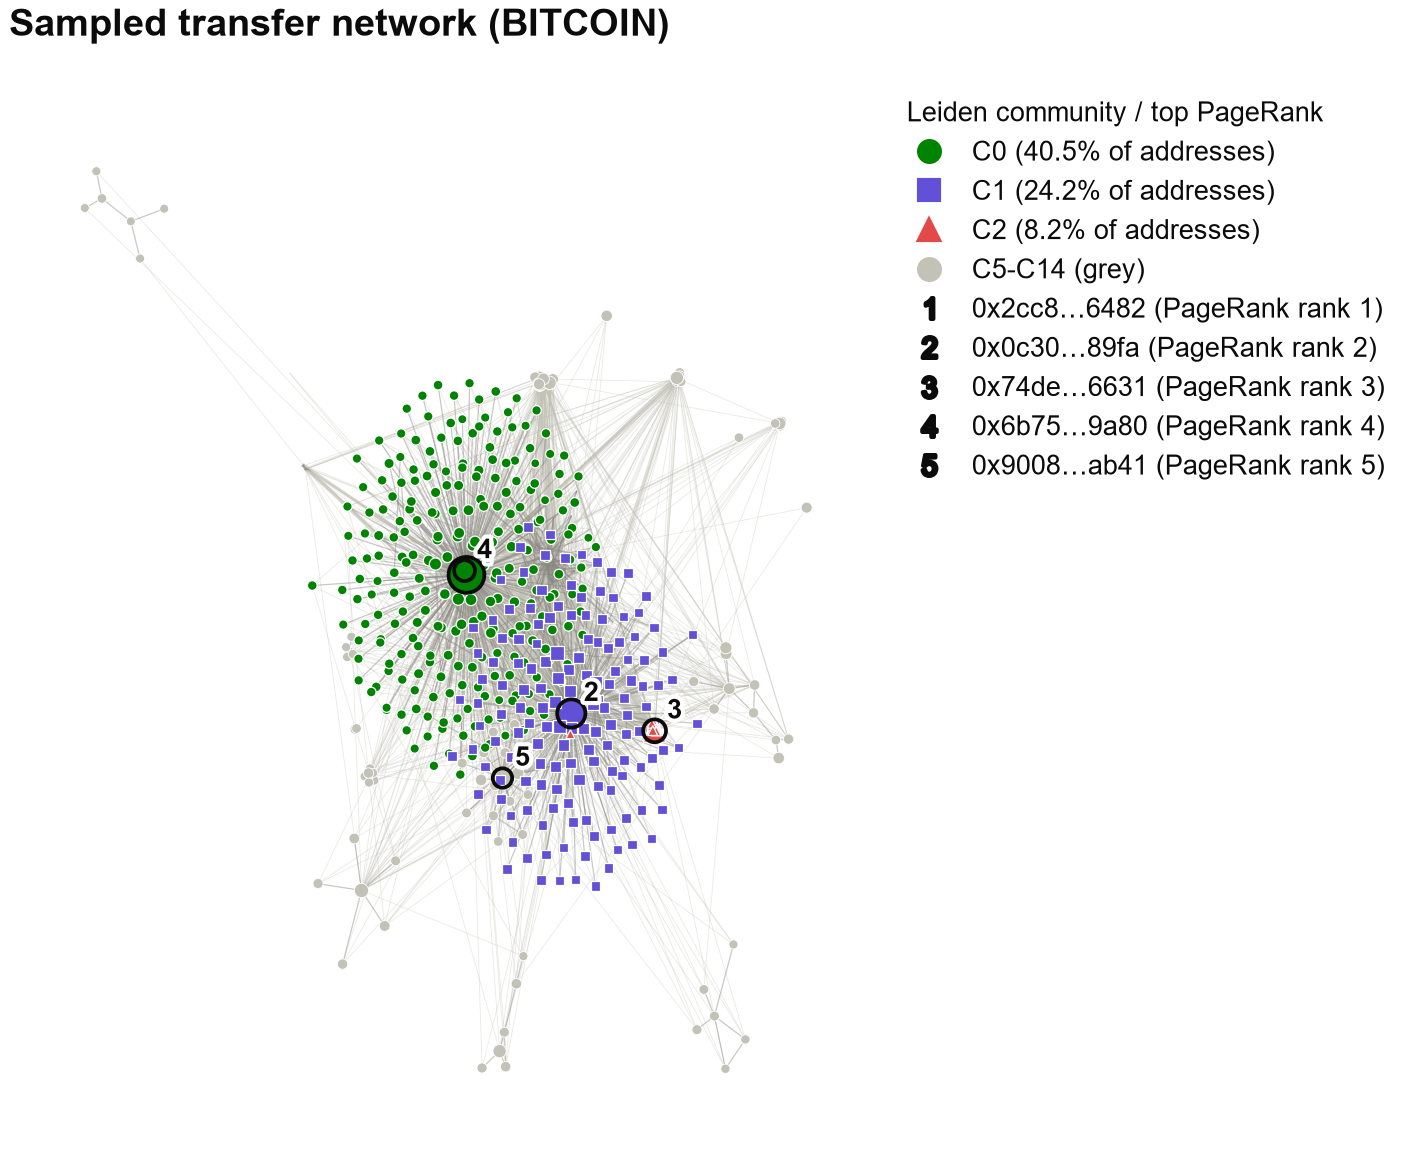
\includegraphics[width=\linewidth]{../../reports/study_A/runs/SNA/figures/fig17_3_network_sample_BITCOIN}
        \caption{BITCOIN ($613$ di $32\,047$ indirizzi)}
        \label{fig:fig17_3_network_sample_bitcoin}
    \end{subfigure}\hfill
    \begin{subfigure}[b]{0.49\linewidth}
        \centering
        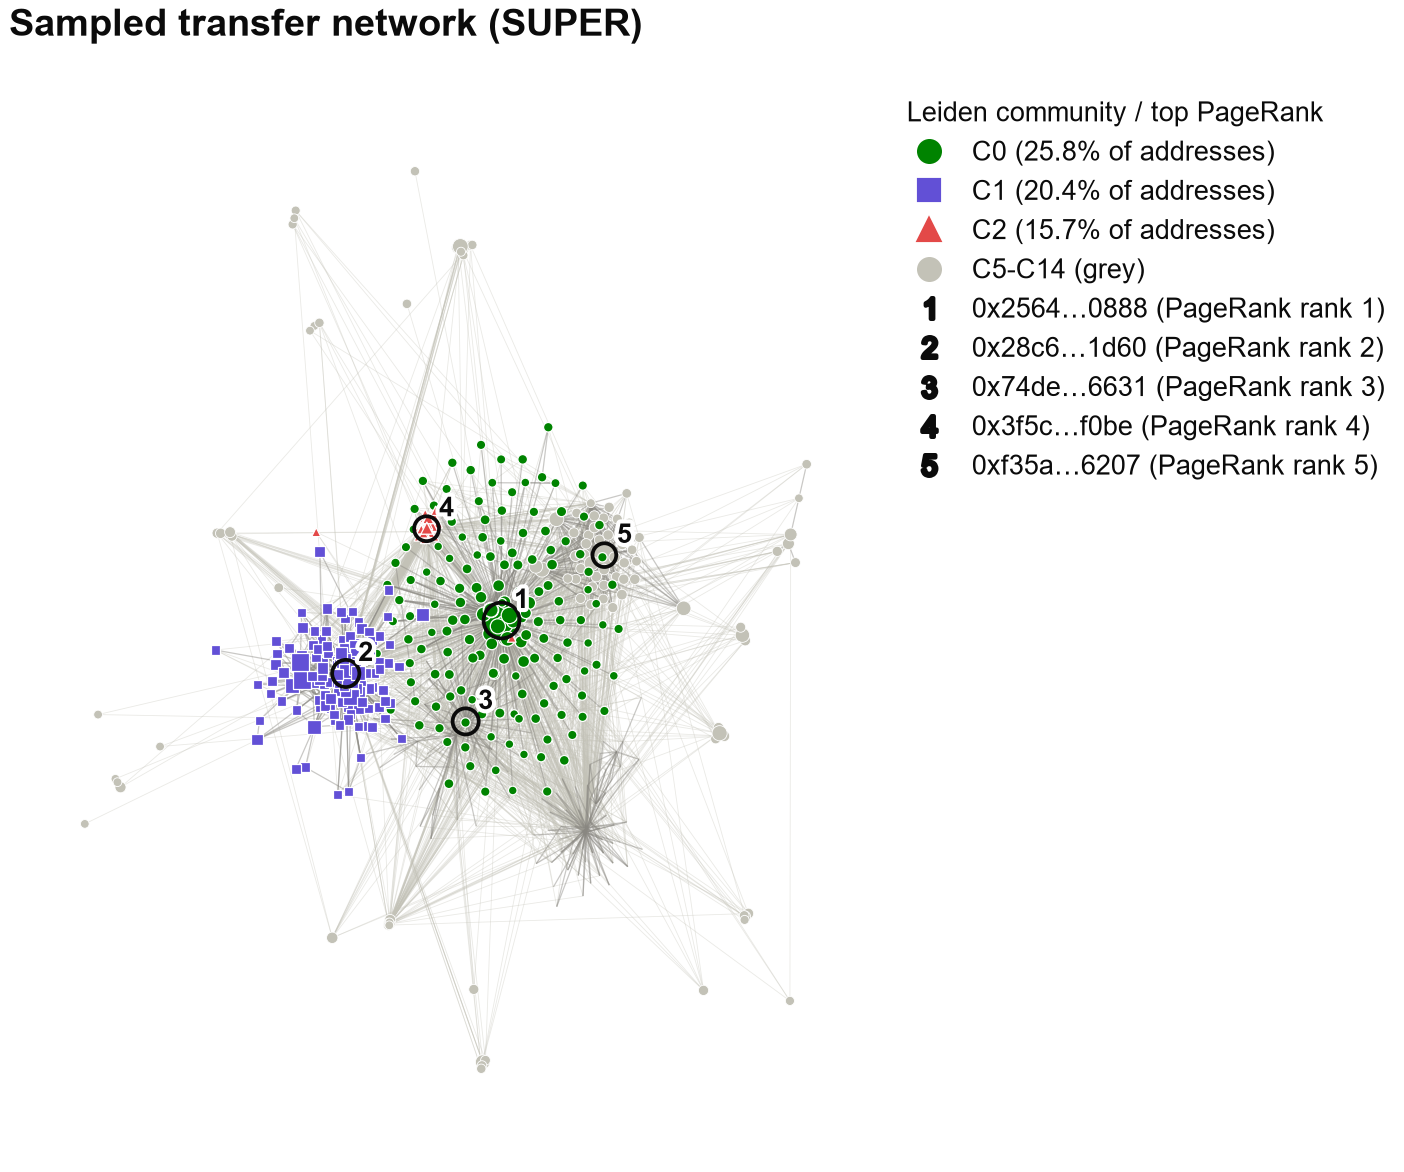
\includegraphics[width=\linewidth]{../../reports/study_A/runs/SNA/figures/fig17_4_network_sample_SUPER}
        \caption{SUPER ($614$ di $82\,994$ indirizzi)}
        \label{fig:fig17_4_network_sample_super}
    \end{subfigure}
    \caption{Sottografi campionati in modo deterministico: gli indirizzi
    con forza maggiore delle 15 community Leiden più grandi, in proporzione
    alla dimensione di ciascuna. Colori: community principali; area dei nodi
    $\propto \sqrt{\text{PageRank}}$; numerati i cinque indirizzi con
    PageRank più alto.}
    \label{fig:fig17_network_sample}
\end{figure}

Ogni \textbf{community} principale si \textbf{raccoglie attorno} a uno o \textbf{pochi
indirizzi} con \textbf{PageRank }\cite{page1999pagerank} molto \textbf{alto}, collegati a molti nodi periferici che hanno
pochi legami tra loro. È la configurazione che produce \textbf{disassortatività e
deficit di triangoli} (Figura~\ref{fig:fig08_small_world}). In SUPER le due
community maggiori formano blocchi ben separati, ciascuno con un proprio hub; in
SWAP e BITCOIN le community si sovrappongono di più attorno ai loro hub.
L'indirizzo \texttt{0x74de\ldots6631} compare tra i primi cinque per PageRank
in tutti e quattro i token (terzo in SWAP, BITCOIN e SUPER, quarto in RARI); si tratta del \textbf{router di scambio} ufficiale di \textbf{MetaMask} (noto come MetaMask Swap Router)\footnote{Secondo l'etichetta pubblica di
Etherscan dell'indirizzo \texttt{0x74de5d4fcbf63e00296fd95d33236b9794016631}.
L'attribuzione si basa su questa sola fonte esterna e non è verificata
indipendentemente.}, che gestisce le operazioni di conversione
dei token e l'instradamento della liquidità tramite aggregatori decentralizzati. Dunque se dovessimo fare un analisi degli indirizzi potremmo tranquillamente andare a verificare quali di questi sono ben conosciuti nella block-chain.
Alcuni indirizzi occupano quindi posizioni centrali in più reti di token.

\subsection{Condivisione degli indirizzi}
Per capire se gli stessi indirizzi compaiono in più token, è stata effettuata questa analisi, che mostra come
le popolazioni dei token si sovrappongono poco.
\begin{figure}[H]
    \centering
    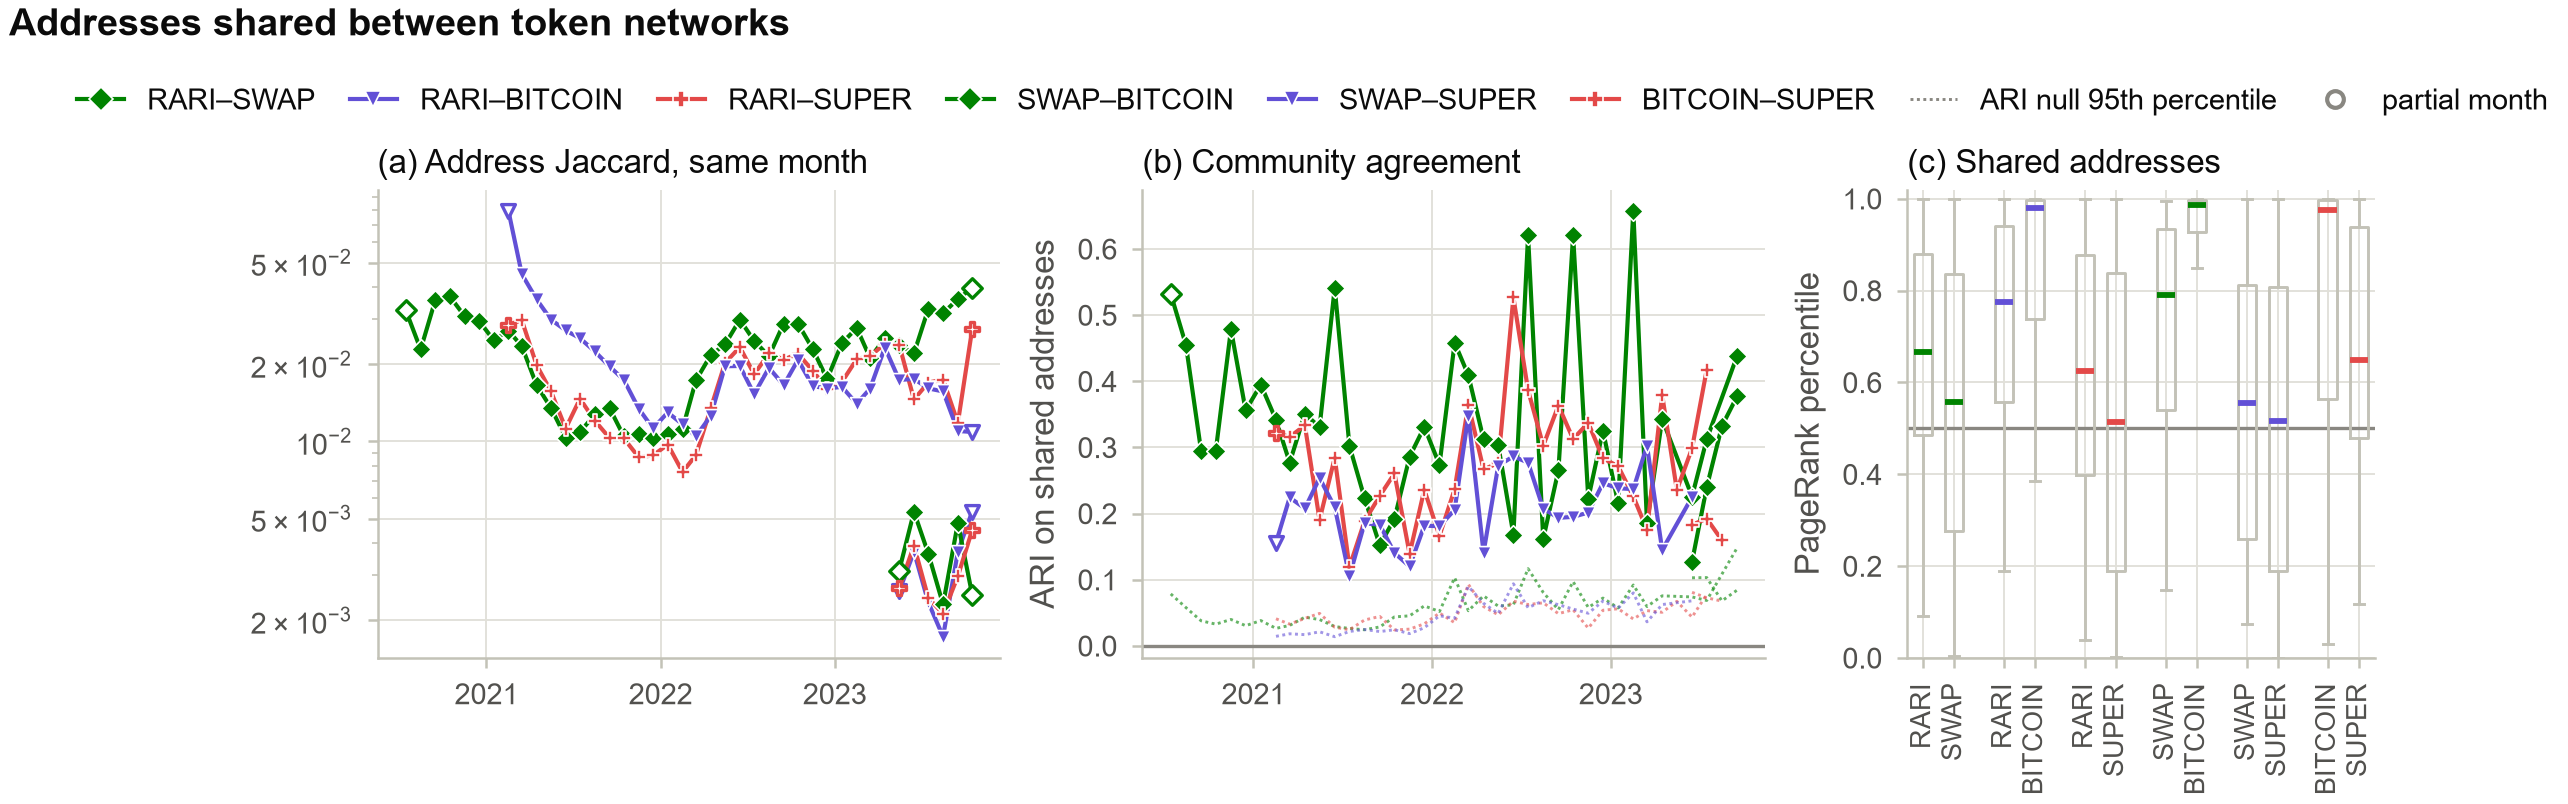
\includegraphics[width=\linewidth]{../../reports/study_A/runs/SNA/figures/fig18_cross_token_overlap}
    \caption{Indirizzi condivisi tra coppie di token: similarità di Jaccard
    degli insiemi di indirizzi nello stesso mese (a); ARI tra le partizioni
    Leiden ristrette agli indirizzi condivisi, con il 95° percentile di 200
    permutazioni (punteggiato) (b); percentile di PageRank degli indirizzi
    condivisi in ciascun token (c).}
    \label{fig:fig18_cross_token_overlap}
\end{figure}
Nello stesso mese la similarità di Jaccard (indirizzi in comune diviso indirizzi nell'unione dei due token) tra RARI, SWAP e SUPER è tra lo $0{,}8\%$ e il 7\%,
e con BITCOIN scende allo $0{,}2$--$0{,}5\%$ (a). Gli indirizzi condivisi, però, non sono
distribuiti a caso. Quando due di essi stanno nella stessa community in un
token, tendono a stare insieme anche nell'altro: l'Adjusted Rand Index
(ARI) \cite{hubert1985ari}, che vale 0 per partizioni indipendenti e 1 per
partizioni identiche, va da $0{,}1$ a
$0{,}65$, quasi sempre sopra il 95° percentile delle permutazioni (b). Inoltre
occupano posizioni più centrali della media: la mediana del loro percentile
di PageRank è sopra $0{,}5$ in tutte le coppie e vicina a $0{,}98$ nella rete
BITCOIN (c). Gli indirizzi attivi su più token sono quindi una minoranza
strutturalmente centrale, e si può idealmente pensare a degli attori precisi come exchange o router.

\subsection{Condivisione delle community}
Le matrici seguenti precisano il risultato della Figura~\ref{fig:fig18_cross_token_overlap}b.
\begin{figure}[H]
    \centering
    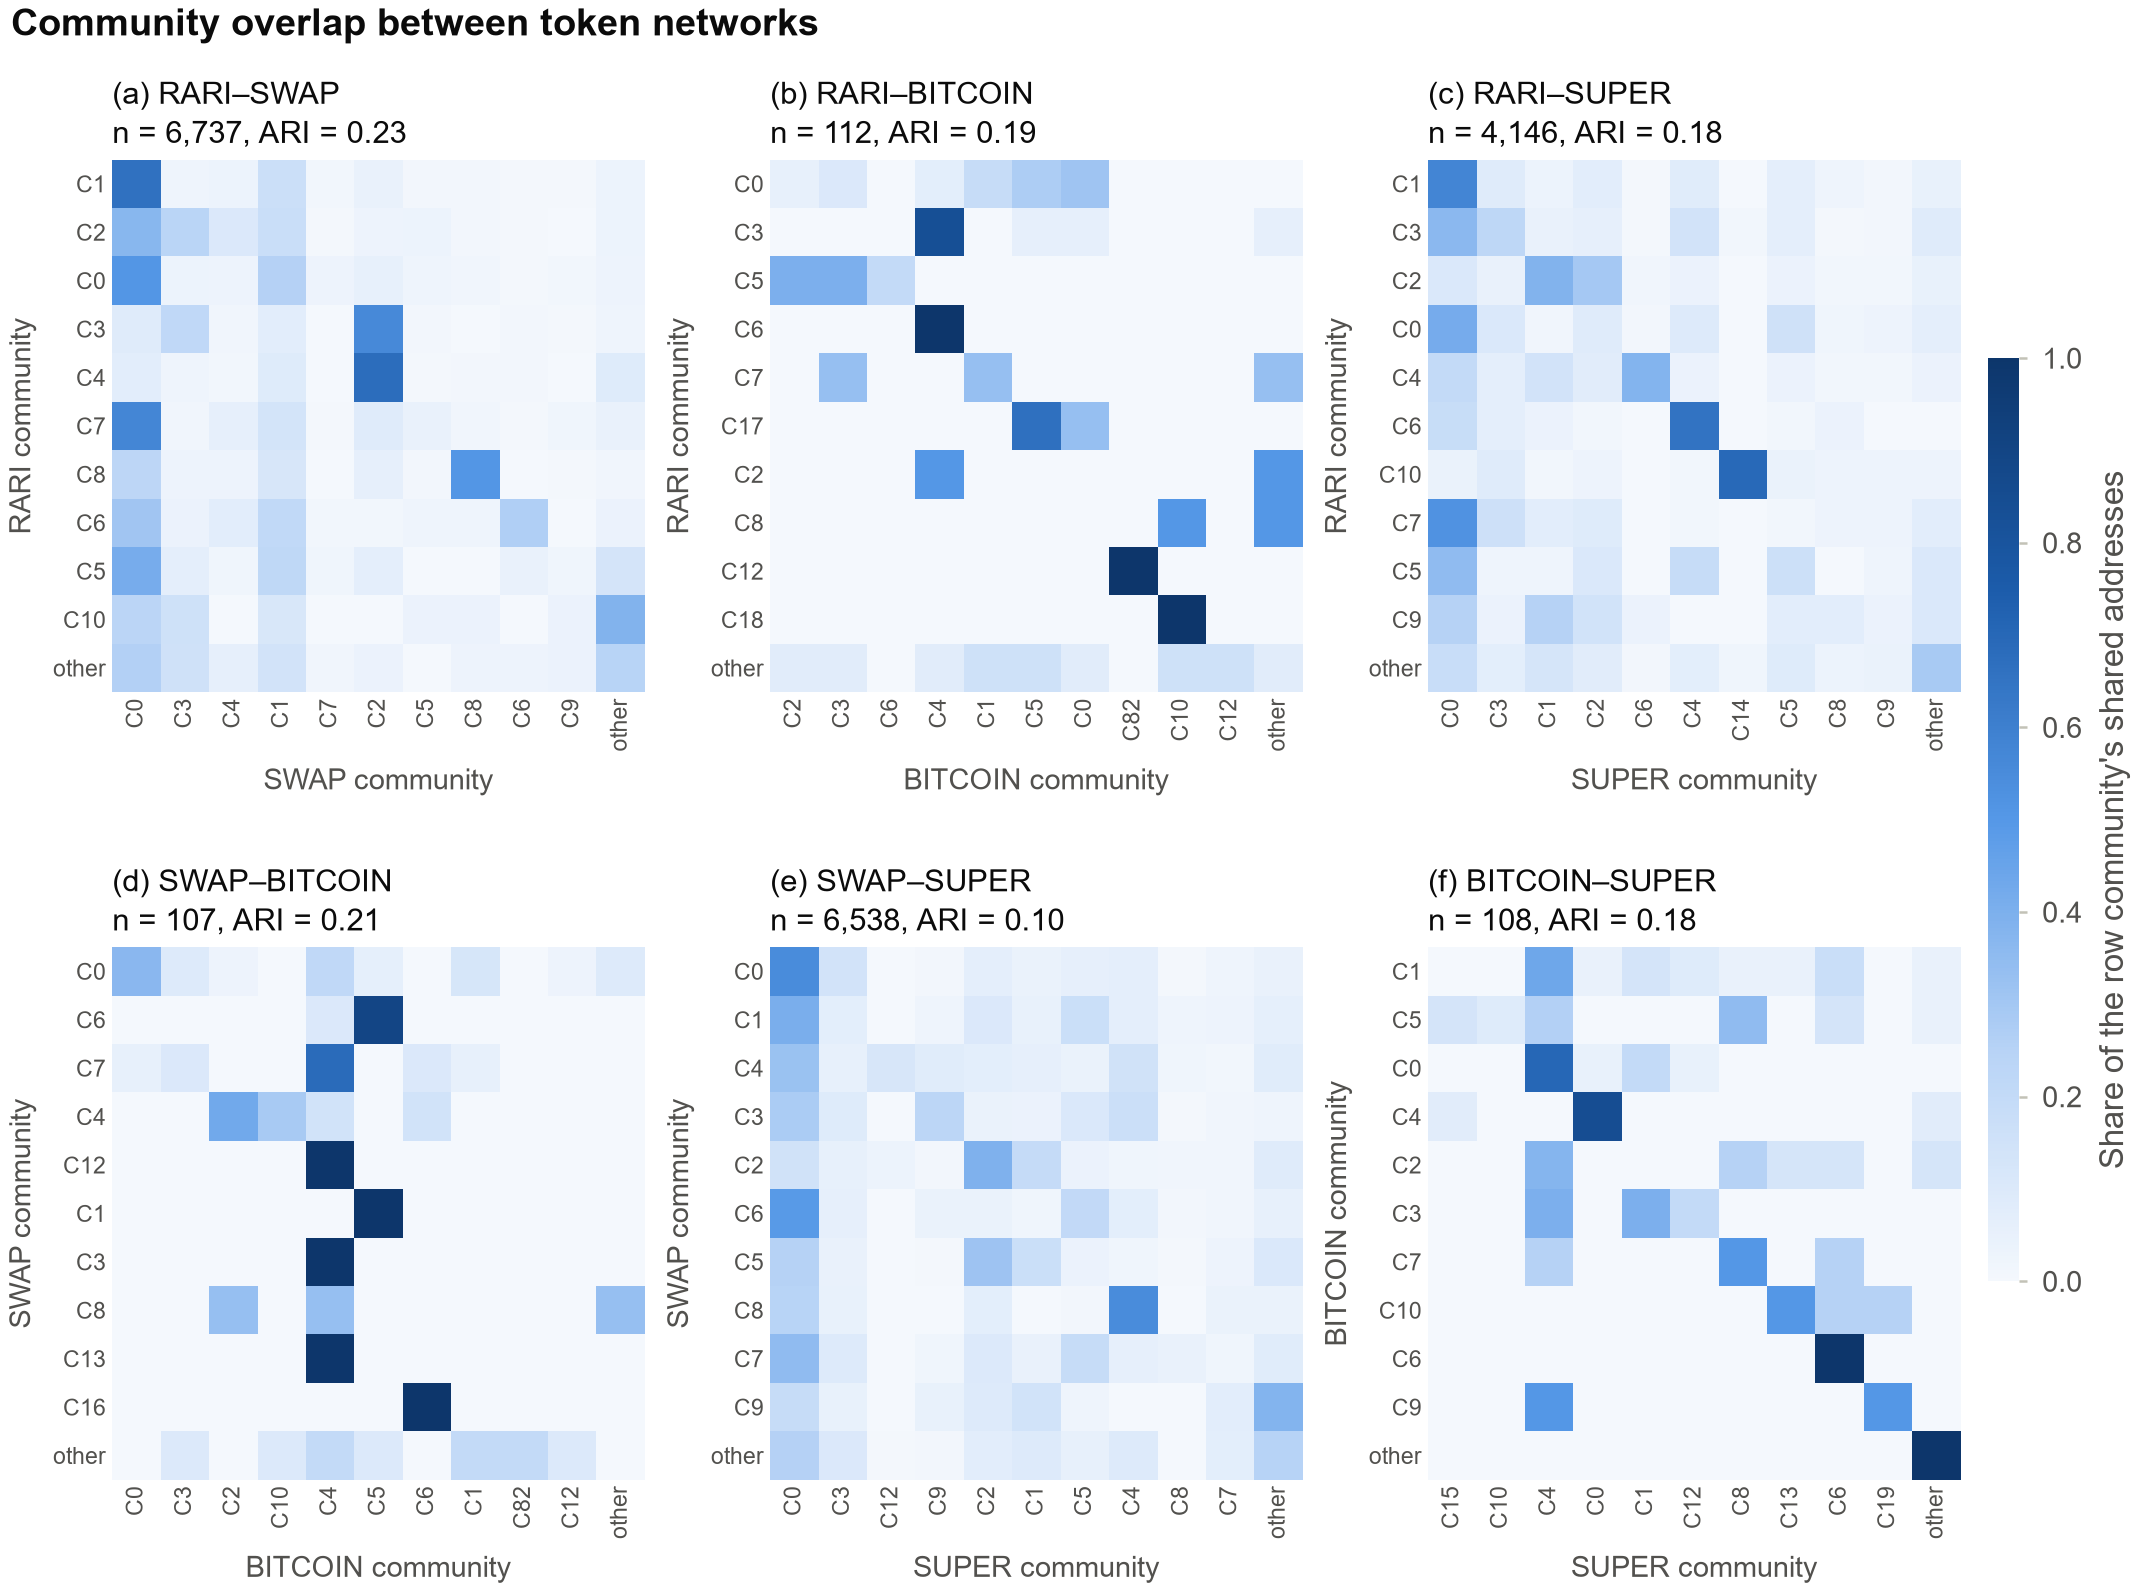
\includegraphics[width=\linewidth]{../../reports/study_A/runs/SNA/figures/fig19_community_overlap}
    \caption{Corrispondenza tra community per ogni coppia di token, sugli
    indirizzi attivi in entrambe nel periodo comune. Ogni cella è la quota
    degli indirizzi condivisi della community di riga che cade nella community
    di colonna (le righe sommano a 1). $n$ = indirizzi condivisi; ARI
    calcolato su tutti.}
    \label{fig:fig19_community_overlap}
\end{figure}

Nelle coppie tra RARI, SWAP e SUPER ($n$, numero di indirizzi condivisi, tra $4\,146$ e $6\,737$) molte righe
si concentrano su un'unica colonna, quasi sempre la community maggiore
dell'altro token: buona parte degli indirizzi condivisi confluisce nel gruppo
principale di entrambe le reti. Accanto a questo compaiono alcune
corrispondenze uno-a-uno nette tra community minori, ad esempio
RARI~C3/C4 $\to$ SWAP~C2 e RARI~C10 $\to$ SUPER~C14. La concordanza
complessiva è moderata (ARI tra $0{,}10$ per SWAP--SUPER e $0{,}23$ per
RARI--SWAP). Le coppie con BITCOIN mostrano diagonali più marcate, ma su
appena 107--112 indirizzi condivisi, quindi vanno lette con cautela.


%-------------- CAPITOLO 3 LINK PREDICTION ---------------------------------


\newpage
\section{Link prediction sul token SWAP}\label{sec:studioB}
Questo studio ha l'obiettivo di comprendere la risposta a un'unica domanda: \emph{quanta parte
della capacità di prevedere un nuovo legame deriva dal sapere solo
chi è attivo, e quanta dalla struttura che lega una specifica
sorgente ai suoi destinatari}.\\
Ogni analisi isola un aspetto diverso di questa distinzione: costruzione del compito, confronto con una baseline di
sola popolarità, difficoltà dei negativi, stabilità dell'addestramento e
distribuzione del rango.

Per ogni settimana target $t$ il \emph{grafo della storia} contiene tutte
le coppie dirette $(u, v)$ con almeno un trasferimento in una settimana
precedente a $t$, e gli \emph{indirizzi della storia} sono quelli attivi
prima di $t$. Un \textbf{positivo} è una coppia il cui primo trasferimento
cade in $t$, con entrambi gli indirizzi già nella storia. I modelli
assegnano un punteggio a ogni coppia ordinata usando solo il grafo della
storia:
\begin{itemize}
    \item \emph{Dst popularity}: trasferimenti ricevuti da $v$ nelle 4
    settimane precedenti, indipendentemente da $u$;
    \item \emph{Preferential Attachment}: grado uscente di $u$ per grado
    entrante di $v$;
    \item \emph{Common Neighbours}: numero di vicini comuni
    nella proiezione non diretta \cite{libennowell2007linkprediction};
    \item \emph{Node2Vec} \cite{grover2016node2vec}: prodotto scalare tra
    gli embedding dei due nodi, appresi con random walk biased e
    ricalcolati ogni 4 settimane. La coppia $(p, q)$ è scelta per AP sui
    negativi uniformi di validazione tra $(0{,}25;\,1)$, $(1;\,1)$,
    $(0{,}25;\,4)$, $(1;\,4)$ e $(4;\,4)$, dove $(1;\,1)$ equivale a DeepWalk;
    è stata selezionata $p = 0{,}25$, $q = 4$, cioè walk che restano vicine
    al nodo di partenza;
    \item \emph{GraphSAGE} \cite{hamilton2017graphsage} e \emph{GAT}
    \cite{velickovic2018gat}: 3 strati che aggregano i vicini separatamente
    lungo gli archi in entrata e in uscita, partendo da 12 feature di nodo
    calcolate sulla storia (gradi, conteggi e volumi inviati e ricevuti,
    PageRank, clustering, età, tempo dall'ultima attività, attività
    recente). Un \textbf{MLP} sulla concatenazione ordinata degli embedding di $u$ e
    $v$ \textbf{produce} il \textbf{punteggio}, per cui $(u, v)$ e $(v, u)$ hanno punteggi
    diversi. Entrambi sono addestrati con 5 negativi uniformi per positivo
    ed early stopping sull'AP dei negativi uniformi di validazione;
    \item \emph{GraphSAGE} e \emph{GAT} \emph{con negativi misti}: stessa
    architettura, ma ogni negativo di addestramento è estratto con
    probabilità $1/2$ dal pool uniforme o da quello recente, e l'early
    stopping usa la media dell'AP di validazione sui due tipi di negativi
    (Sezione~\ref{sec:negativi_misti}).
\end{itemize}
Le metriche per l'analisi dei risultati sono:
\begin{itemize}
    \item L'\textbf{Average Precision} (AP) è l'area sotto la
    curva precision--recall calcolata su tutte le coppie insieme, e quindi
    confronta anche coppie con sorgenti diverse.
    \item Il \emph{rango} del positivo è la sua posizione tra i 51 candidati della stessa sorgente (il positivo e
    i suoi 50 negativi), con le parità contate per metà.
    \item  Il \textbf{Mean Reciprocal Rank} (MRR) è la media di $1/\text{rango}$, e
    \textbf{Hits@K} è la quota di \textbf{positivi} con \textbf{rango $\le K$}.
\end{itemize}
\subsection{Analisi}
Il compito è prevedere, per ogni settimana $t$, quali coppie dirette
$(u, v)$ mai osservate prima compaiono in $t$, usando solo i trasferimenti
delle settimane precedenti.

\begin{figure}[H]
    \centering
    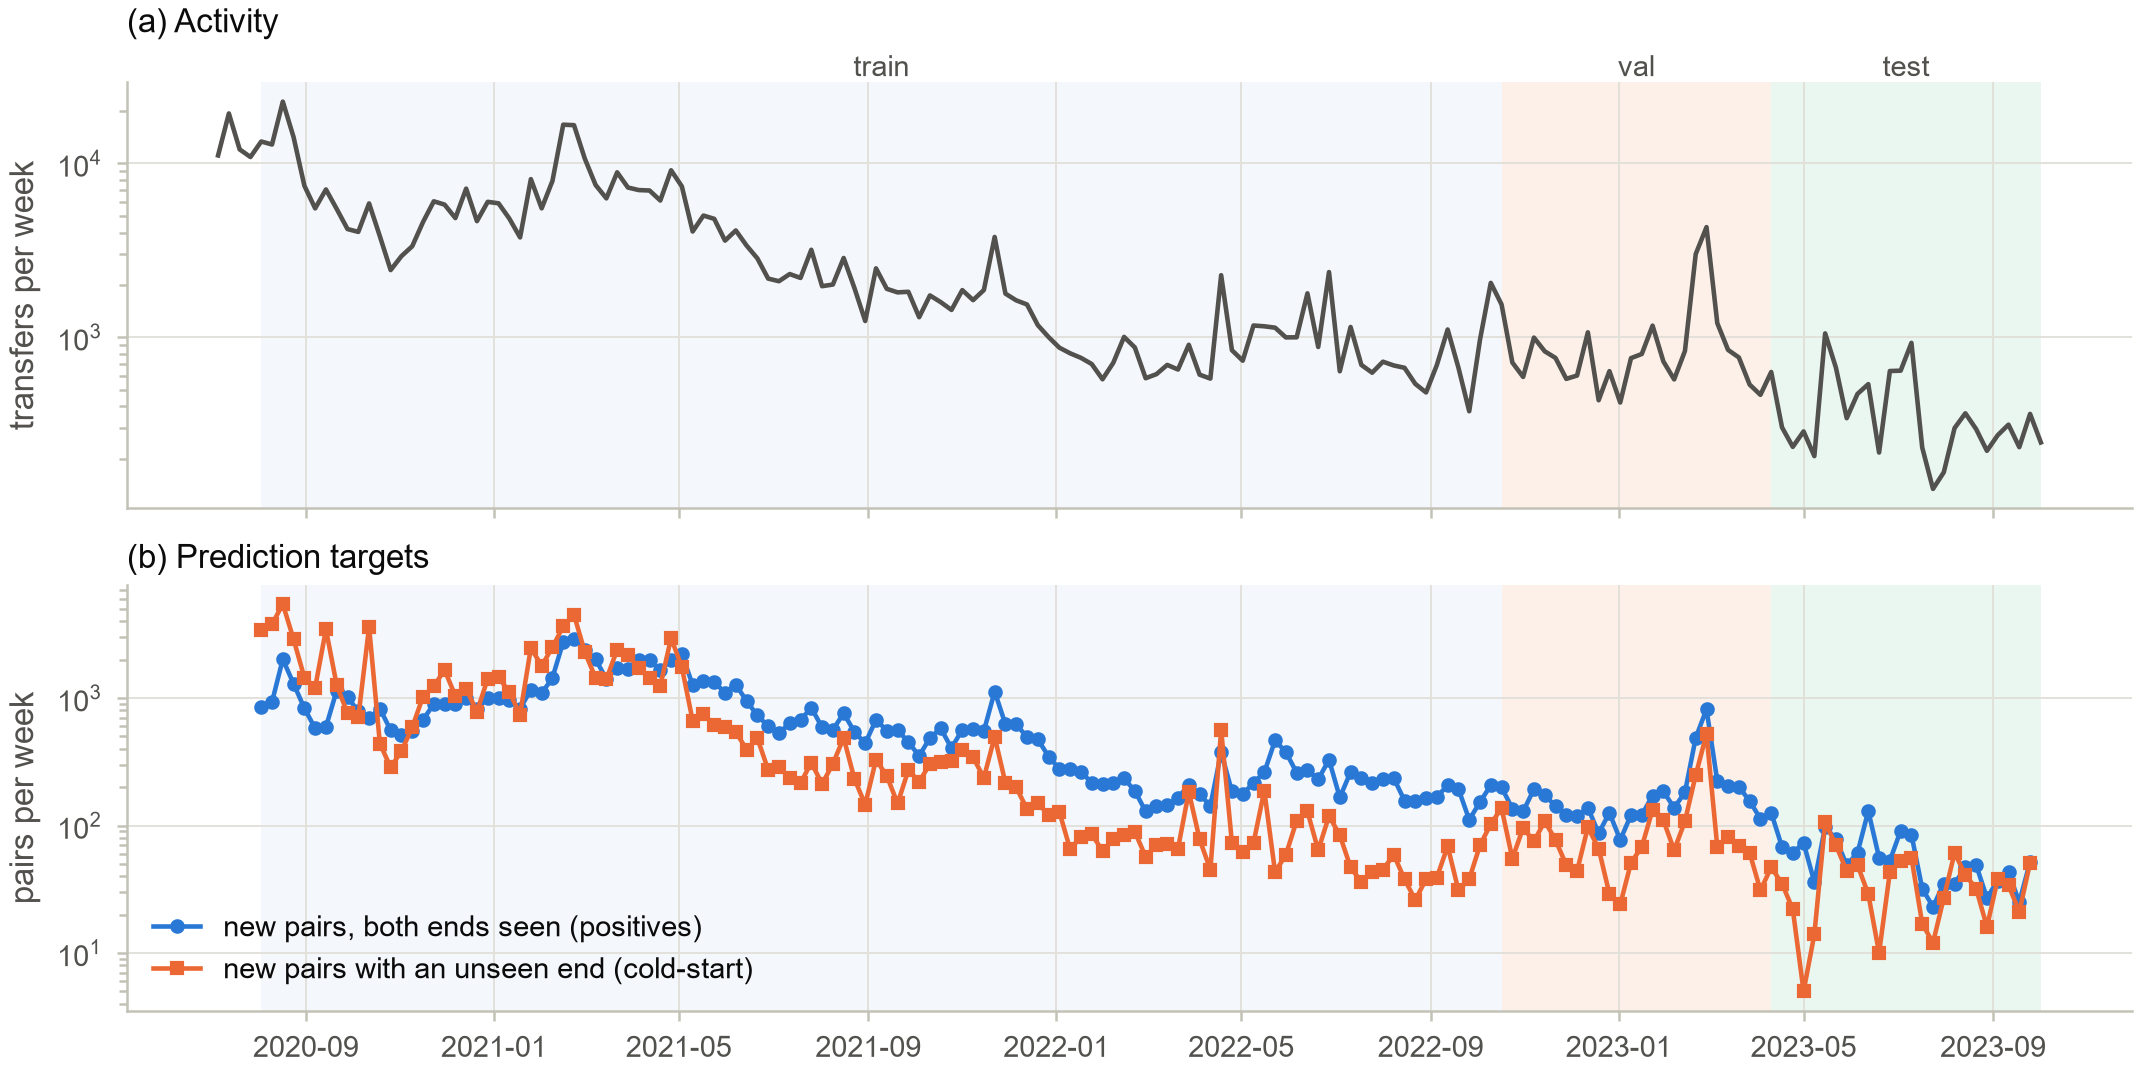
\includegraphics[width=\linewidth]{../../reports/study_B/runs/COMPLETO_2_all/figures/fig1_windows}
    \caption{Settimane disgiunte del token SWAP e split cronologico.
    (a) Trasferimenti unici per settimana (scala logaritmica). (b) Per ogni
    settimana target, nuove coppie dirette con entrambi gli estremi già
    osservati nella storia (positivi) e nuove coppie con almeno un estremo mai
    visto (\emph{cold start}, escluse).}
    \label{fig:fig1_windows}
\end{figure}

Le 170 settimane sono divise in ordine
cronologico: le prime 4 servono solo da storia, seguono 115 settimane di
addestramento (agosto 2020 -- ottobre 2022), 25 di validazione (ottobre
2022 -- aprile 2023) e 25 di test (aprile -- settembre 2023); l'ultima
settimana, coperta solo in parte, è esclusa. L'attività cala da oltre
$10^4$ a poche centinaia di trasferimenti a settimana (a), per cui il test
conta $1\,470$ positivi contro gli $83\,333$ dell'addestramento: i modelli
sono addestrati su un regime molto più denso di quello su cui sono
valutati. Le nuove coppie con un estremo mai visto sono il 51\% del totale
(39\% nel test) e non hanno alcuna rappresentazione nella storia; i
risultati valgono quindi solo per coppie tra indirizzi già attivi. È la
conseguenza diretta dell'alto ricambio osservato nello Studio A
(Figura~\ref{fig:fig13_turnover}). Ogni positivo $(u, v)$ è confrontato con
50 negativi $(u, v')$ con la stessa sorgente, estratti uniformemente tra gli
indirizzi della storia (\emph{uniform}) oppure tra quelli che hanno ricevuto
almeno un trasferimento nelle 4 settimane precedenti (\emph{recent}).\\ \emph{Le
metriche misurano quindi se il modello ordina il vero destinatario di $u$
sopra 50 alternative.}

\begin{figure}[H]
    \centering
    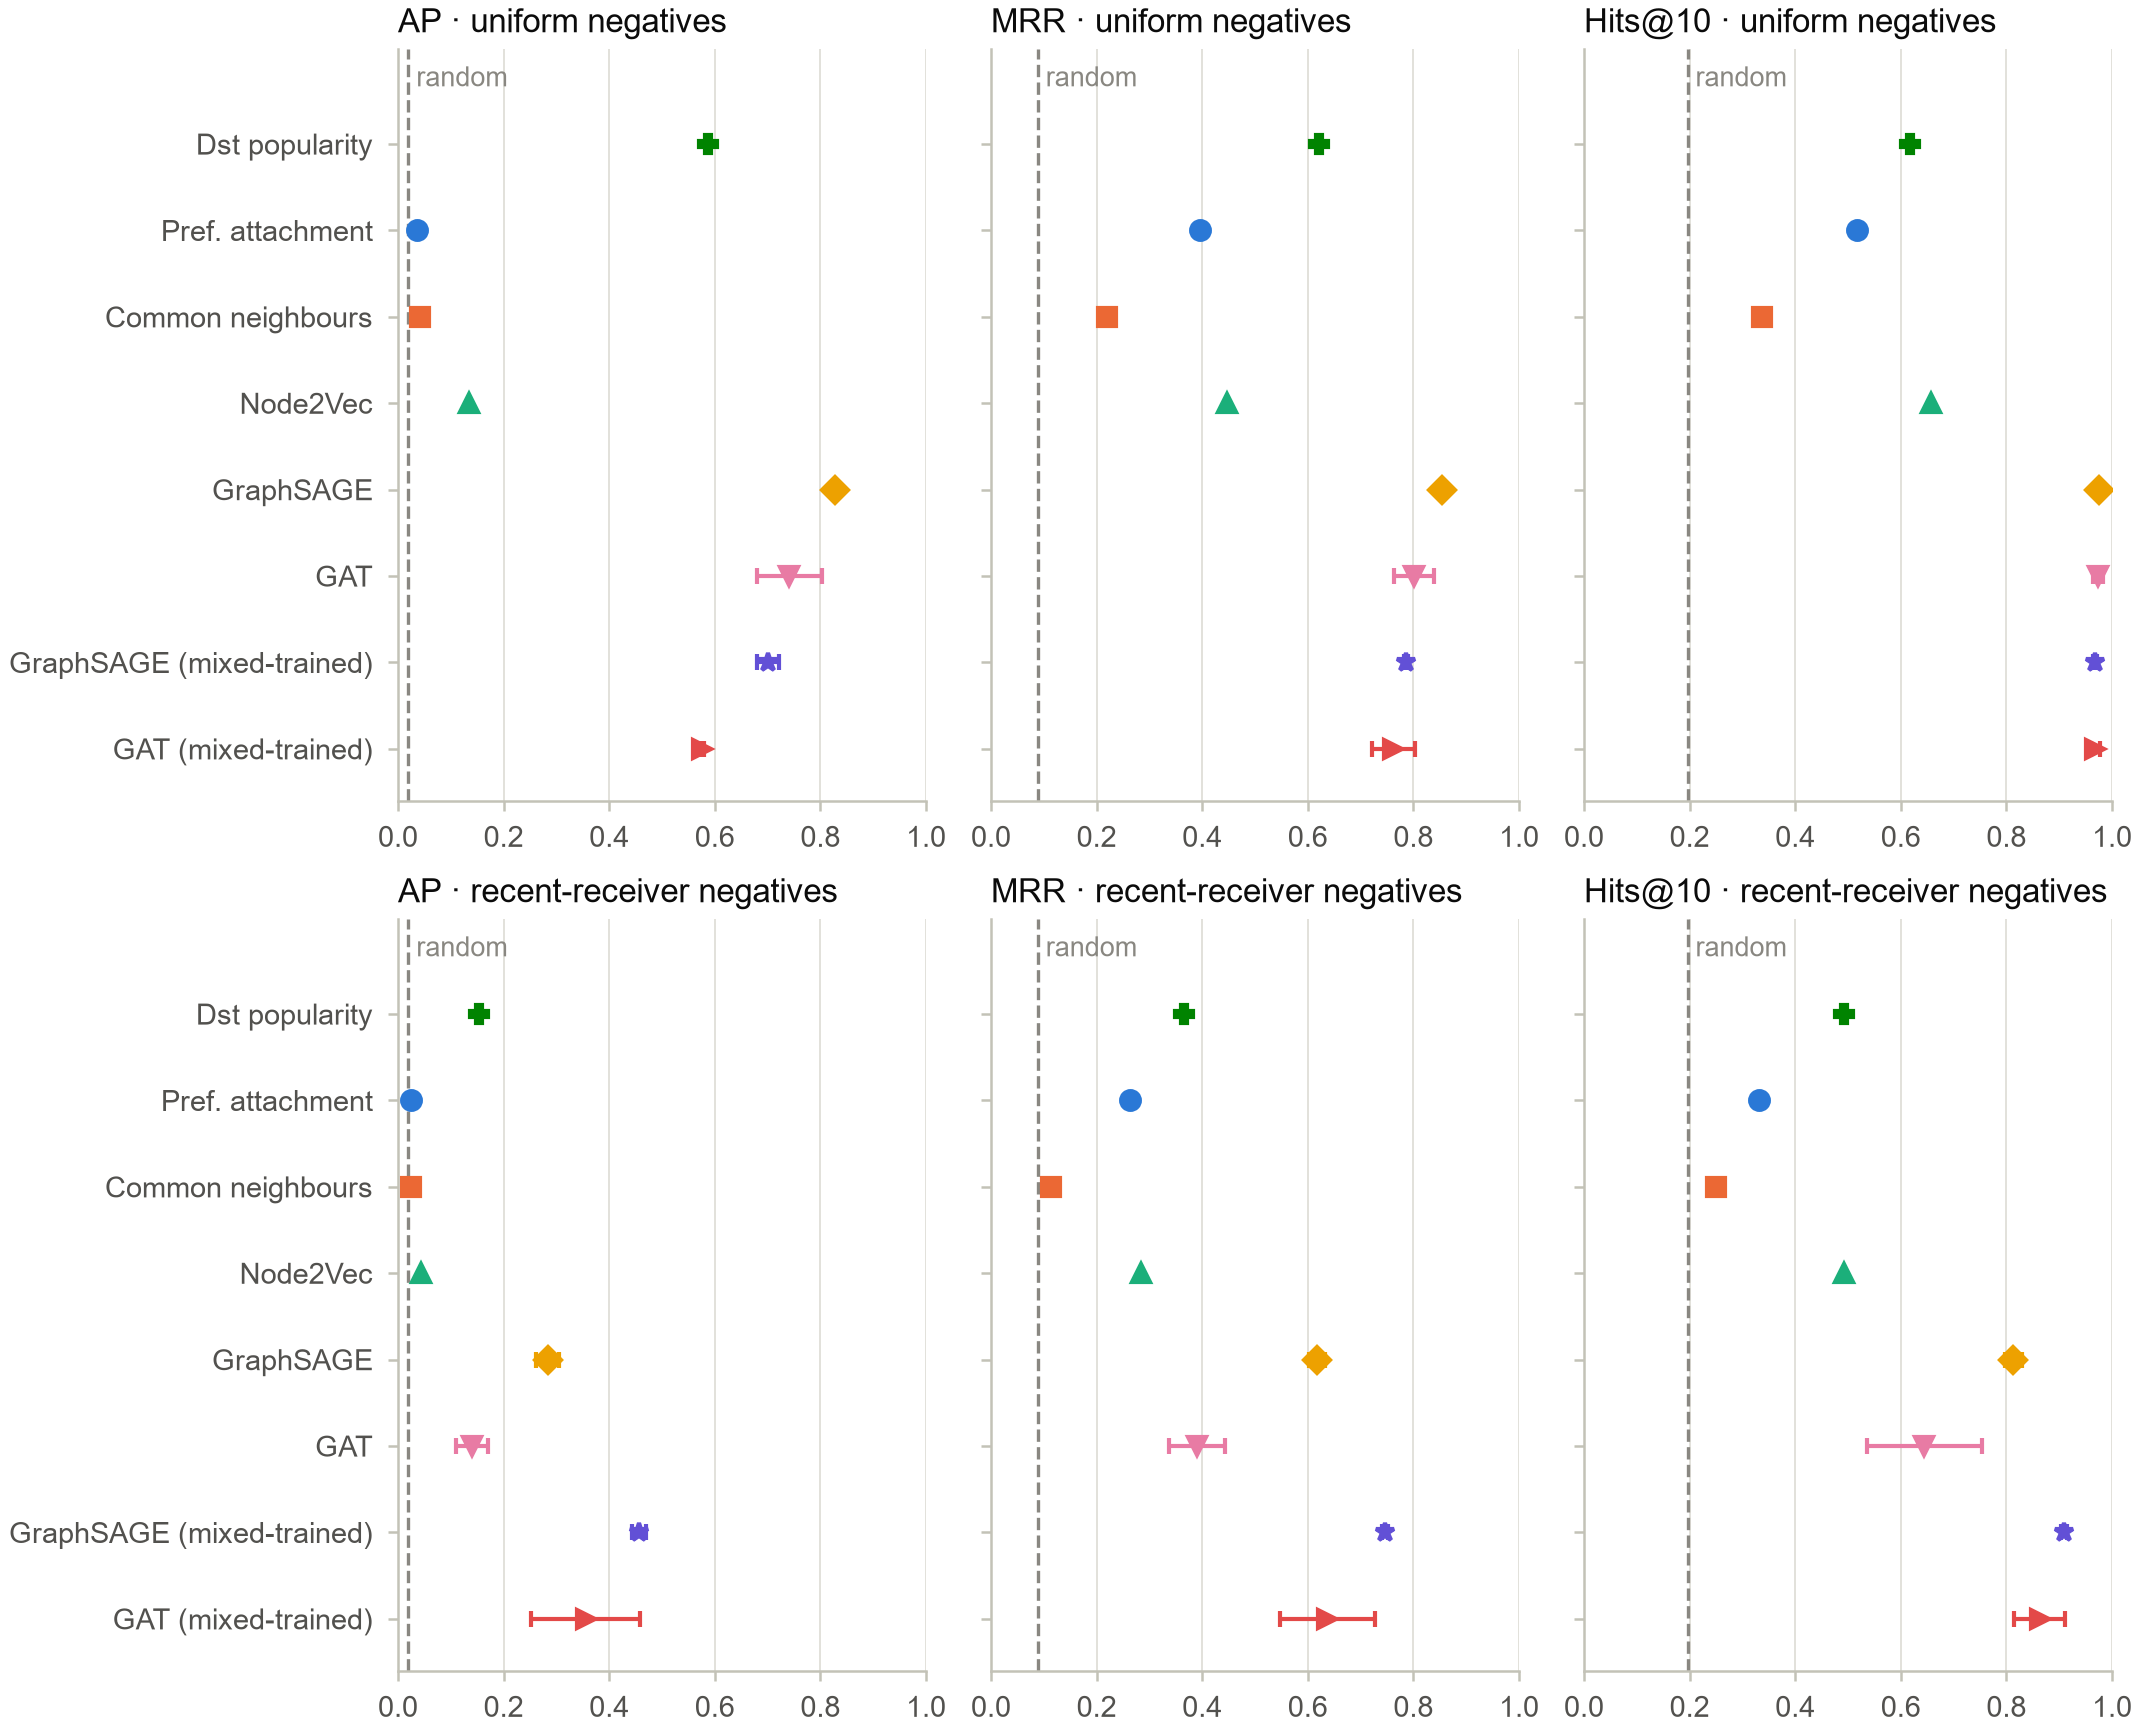
\includegraphics[width=\linewidth]{../../reports/study_B/runs/COMPLETO_2_all/figures/fig2_model_comparison}
    \caption{Prestazioni sul test con negativi uniformi (sopra) e recenti
    (sotto): AP, MRR e Hits@10. Per GraphSAGE e GAT, anche nelle varianti con
    negativi misti (Sezione~\ref{sec:negativi_misti}), media $\pm$ deviazione
    standard su 3 seed. Linea tratteggiata: valore atteso di un ordinamento
    casuale (AP $= 1/51 \approx 0{,}02$, MRR $\approx 0{,}09$, Hits@10
    $= 10/51 \approx 0{,}20$).}
    \label{fig:fig2_model_comparison}
\end{figure}

Il \textbf{riferimento} da battere è \textbf{Dst popularity}, che assegna a $(u, v)$ il
numero di trasferimenti ricevuti da $v$ nelle 4 settimane precedenti e
ignora $u$: misura quanto si ottiene sapendo solo \emph{chi} è attivo. Con
negativi uniformi questa baseline raggiunge già AP $0{,}59$ e MRR $0{,}62$,
mentre preferential attachment, common neighbours e Node2Vec restano sotto
(AP $\le 0{,}14$, MRR tra $0{,}22$ e $0{,}45$). Rispetto alle walk uniformi
($p = q = 1$), le walk biased di Node2Vec alzano l'AP (da $0{,}09$ a
$0{,}14$) ma abbassano la MRR (da $0{,}55$ a $0{,}45$), senza cambiare il
quadro. Common neighbours è vicino
al caso perché nella struttura a stella descritta nello Studio A sorgente e
destinatario hanno raramente vicini in comune.\\ Tra i modelli addestrati
con negativi uniformi, solo GraphSAGE (AP $0{,}83$, MRR $0{,}86$, Hits@10
$0{,}98$) e GAT (AP $0{,}74$, MRR $0{,}80$) superano la baseline. Con negativi recenti tutte le metriche calano: GraphSAGE scende
ad AP $0{,}28$ e MRR $0{,}62$ ma resta sopra Dst popularity ($0{,}15$ e
$0{,}37$), mentre GAT si porta al livello della baseline (AP $0{,}14$, MRR
$0{,}39$) con ampia variabilità tra seed. Ne seguono due conclusioni: gran
parte delle prestazioni con negativi uniformi deriva dal distinguere
destinatari attivi da indirizzi dormienti, e solo GraphSAGE dimostra di
sapere qualcosa su \emph{a chi} una sorgente invierà. Le varianti con
negativi misti, discusse nella Sezione~\ref{sec:negativi_misti}, spostano
questo equilibrio: perdono qualcosa sui negativi uniformi e guadagnano su
quelli recenti.

Il vantaggio di GraphSAGE è stabile nel tempo. Supera Dst
popularity in tutte le 25 settimane di test con entrambi i tipi di negativi,
con un guadagno medio di AP di $+0{,}24$ (uniformi) e $+0{,}13$ (recenti) e
di MRR di $+0{,}25$ e $+0{,}24$. GAT la supera in tutte le settimane con
negativi uniformi, ma con negativi recenti solo in 7 settimane su 25 per AP
e in 10 su 25 per MRR (guadagno medio di AP $-0{,}03$): il suo vantaggio non
regge ai negativi difficili.

\begin{figure}[H]
    \centering
    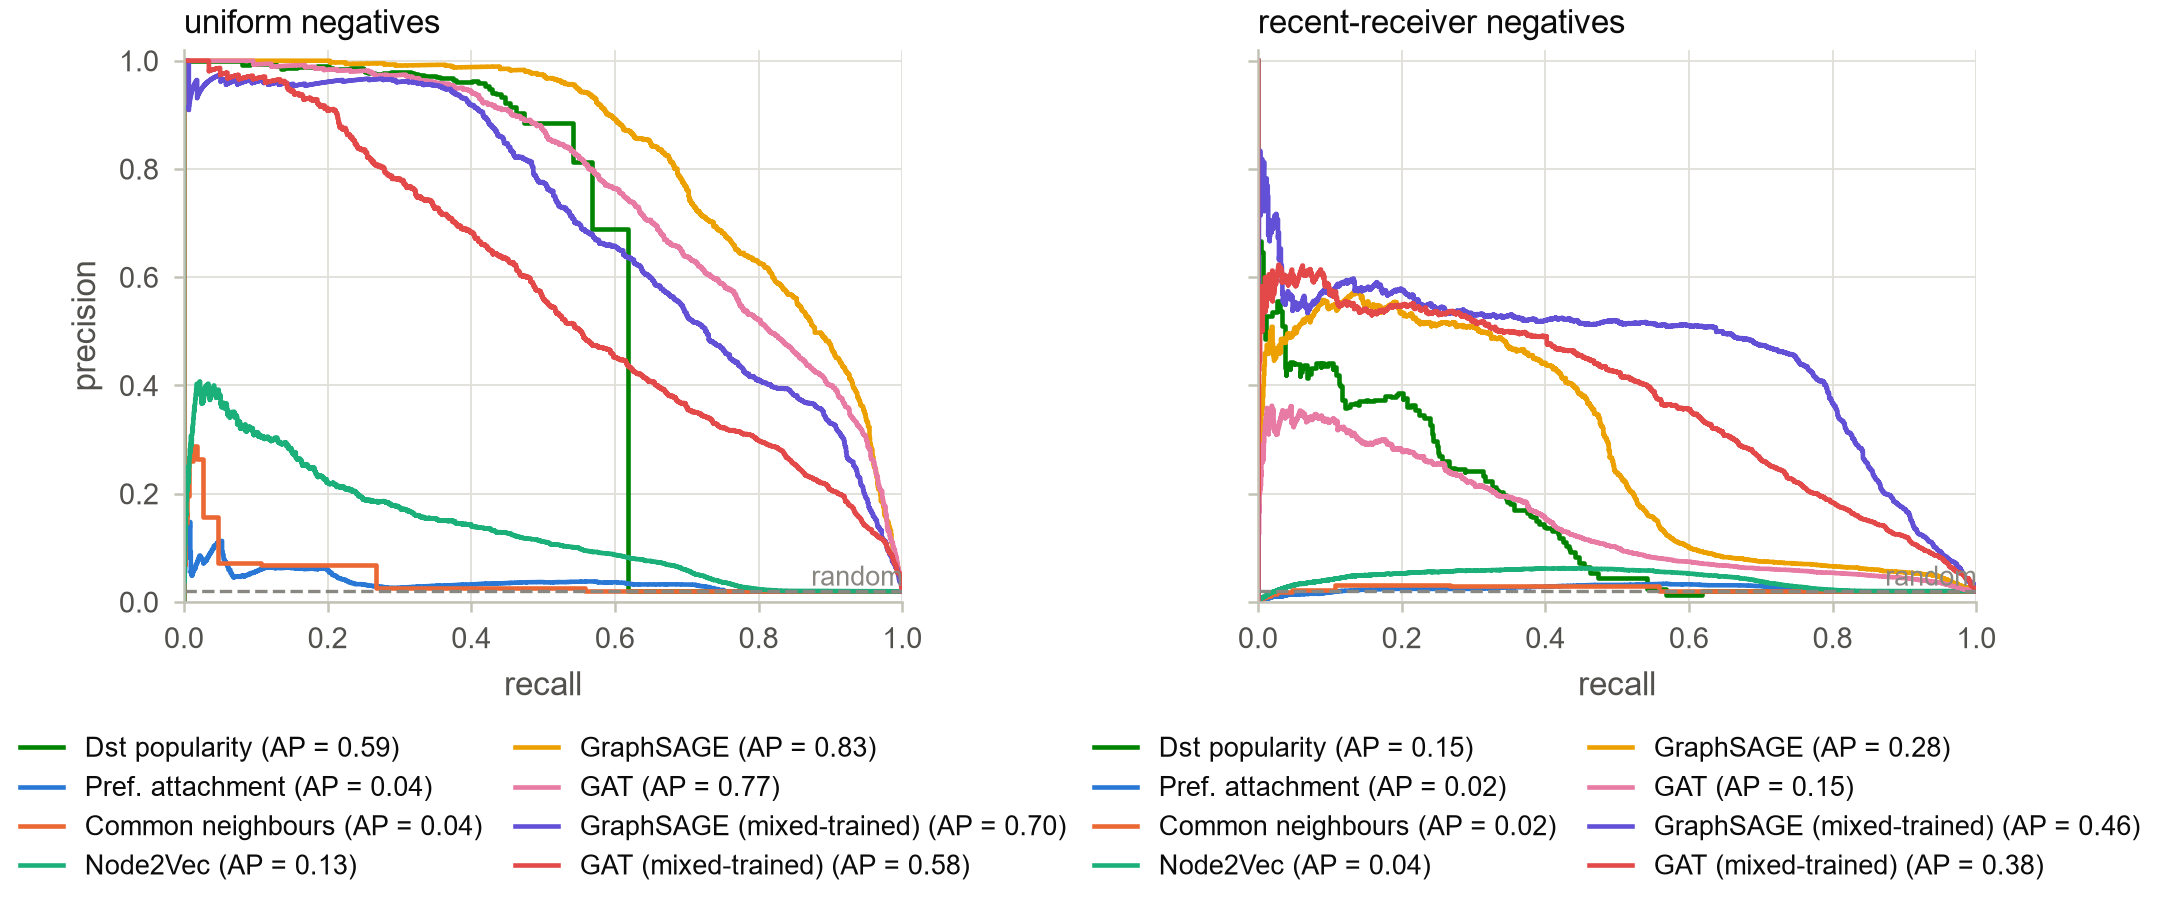
\includegraphics[width=\linewidth]{../../reports/study_B/runs/COMPLETO_2_all/figures/fig3_pr_curves}
    \caption{Curve precision--recall sul test, calcolate su tutte le coppie
    (un positivo ogni 51 coppie). Per GraphSAGE e GAT, anche con negativi
    misti, è mostrato il seed con AP mediana. Linea tratteggiata: precisione di un classificatore casuale.}
    \label{fig:fig3_pr_curves}
\end{figure}

Con negativi uniformi GraphSAGE e GAT, addestrati con negativi uniformi,
mantengono una precisione alta fino a un recall di $0{,}5$ (circa $0{,}97$
e $0{,}87$). Dst popularity ha precisione quasi
perfetta fino a un recall di $0{,}62$ e poi crolla al livello casuale: il
38\% dei positivi ha un destinatario che non ha ricevuto nulla nelle 4
settimane precedenti, ottiene punteggio zero ed è indistinguibile dai
negativi. Con negativi recenti nessun modello supera una precisione di
circa $0{,}65$. GraphSAGE la mantiene sopra $0{,}4$ fino a un recall di
circa $0{,}4$, mentre le varianti con negativi misti restano sopra $0{,}4$
fino a un recall di $0{,}5$ (GraphSAGE misto $0{,}52$, GAT misto $0{,}43$);
le euristiche restano sulla linea casuale.

La \textbf{differenza tra} i due\textbf{ negativi si spiega} con l'\textbf{attività} dei \textbf{destinatari}
candidati. Il vero destinatario era attivo in mediana una settimana prima, i negativi uniformi 117 settimane
prima e quelli recenti 2 settimane prima.
\begin{itemize}
    \item I \textbf{negativi uniformi} sono quasi
    tutti indirizzi \textbf{dormienti }da oltre due\textbf{ anni}, e riconoscerli non richiede di
    capire la struttura: è il problema dei negativi facili descritto da
    Poursafaei et al.\ \cite{poursafaei2022better}.
    \item I \textbf{negativi recenti} hanno
    invece un'attività\textbf{ comparabile} a quella dei \textbf{veri destinatari} e rimuovono
    questa scorciatoia. Circa il 30\% dei veri destinatari era però inattivo da
    più di 20 settimane: per queste coppie anche i \textbf{negativi recenti} sono \textbf{più
    attivi del positivo}, il che spiega parte del \textbf{calo} delle \textbf{prestazioni}.
\end{itemize}

Per entrambi i modelli la loss di addestramento scende rapidamente e si
stabilizza attorno a $0{,}11$ entro circa 50 epoche. GraphSAGE raggiunge un
AP di validazione di circa $0{,}76$ entro 50 epoche e si stabilizza attorno a
$0{,}78$ in tutti e tre i seed, con curve quasi sovrapposte. GAT sale più lentamente e con
forti oscillazioni da un'epoca all'altra; arriva a $0{,}73$--$0{,}78$ solo
dopo 150--350 epoche, con epoche selezionate molto diverse tra i seed. Le
varianti con negativi misti hanno una loss più alta (circa $0{,}14$) e un AP
di validazione più basso ($0{,}66$ GraphSAGE, $0{,}59$--$0{,}65$ GAT),
perché metà dei negativi è difficile; GAT resta instabile e in un seed
raggiunge il limite di 500 epoche senza fermarsi. Come osservabile nel grafico seguente.
\begin{figure}[H]
    \centering
    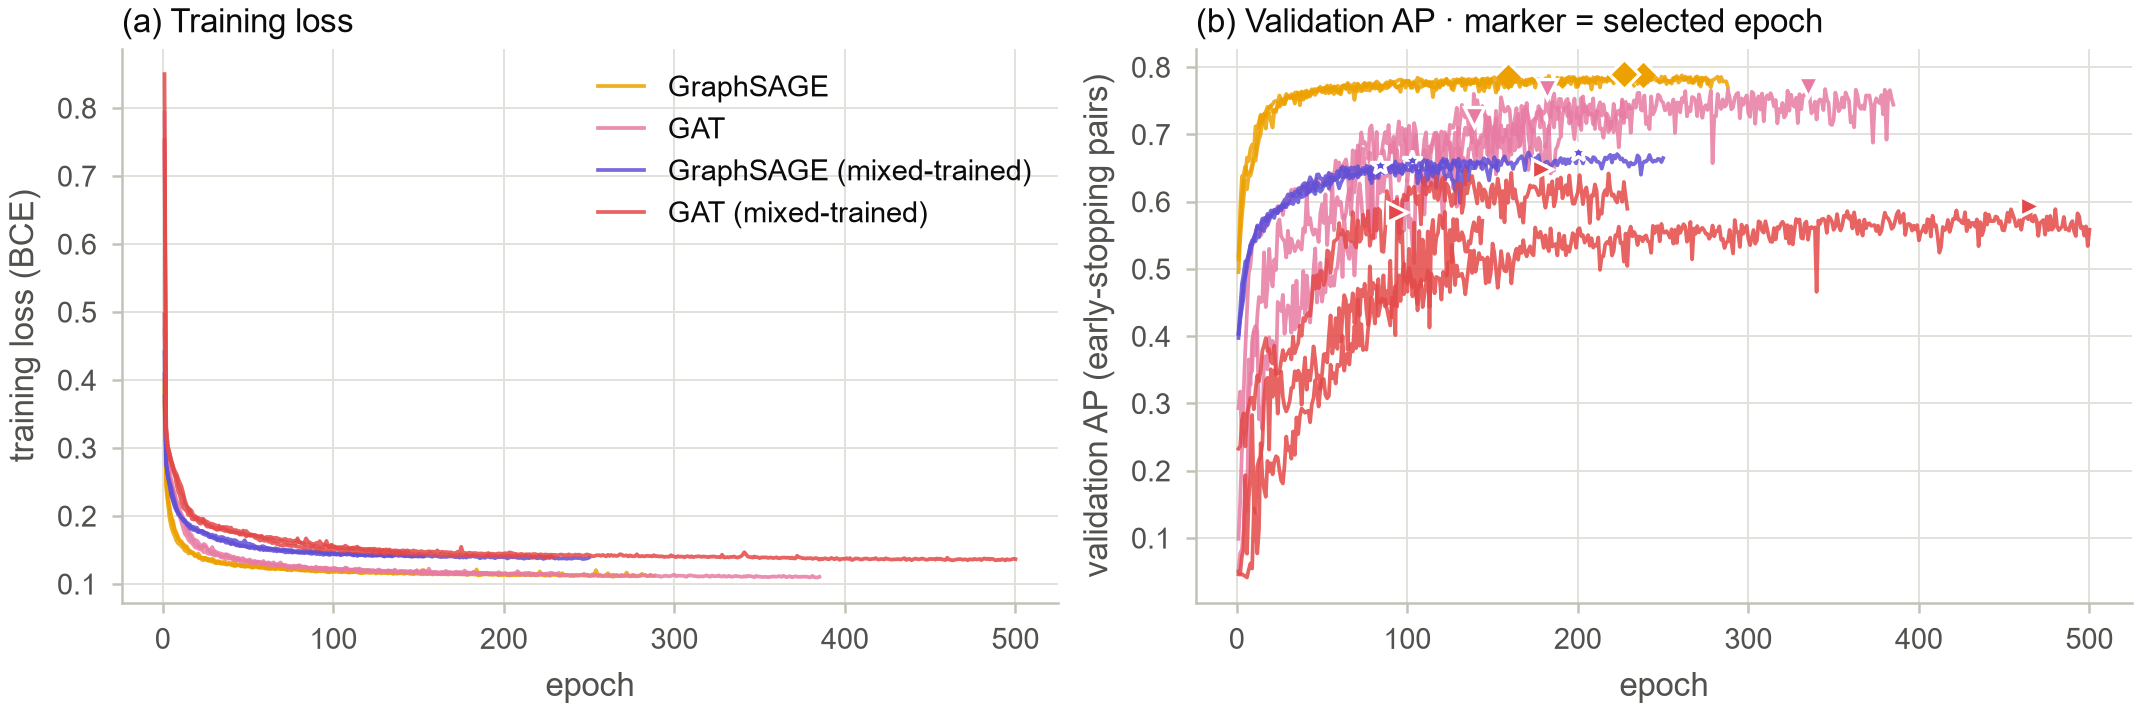
\includegraphics[width=\linewidth]{../../reports/study_B/runs/COMPLETO_2_all/figures/fig6_training_curves}
    \caption{Addestramento di GraphSAGE e GAT, una linea per seed. (a) Loss
    di addestramento (entropia incrociata binaria). (b) AP di validazione
    sulle coppie usate per l'early stopping (negativi uniformi; media di
    uniformi e recenti per le varianti con negativi misti); il marcatore
    indica l'epoca selezionata dall'early stopping (pazienza 50 epoche).}
    \label{fig:fig6_training_curves}
\end{figure}

Poiché  la loss di addestramento resta piatta mentre l'AP di validazione oscilla,
l'instabilità di GAT sembra legata all'ottimizzazione più che a un
sovradattamento, ed è all'origine della sua variabilità tra seed in
Figura~\ref{fig:fig2_model_comparison}.

\begin{figure}[H]
    \centering
    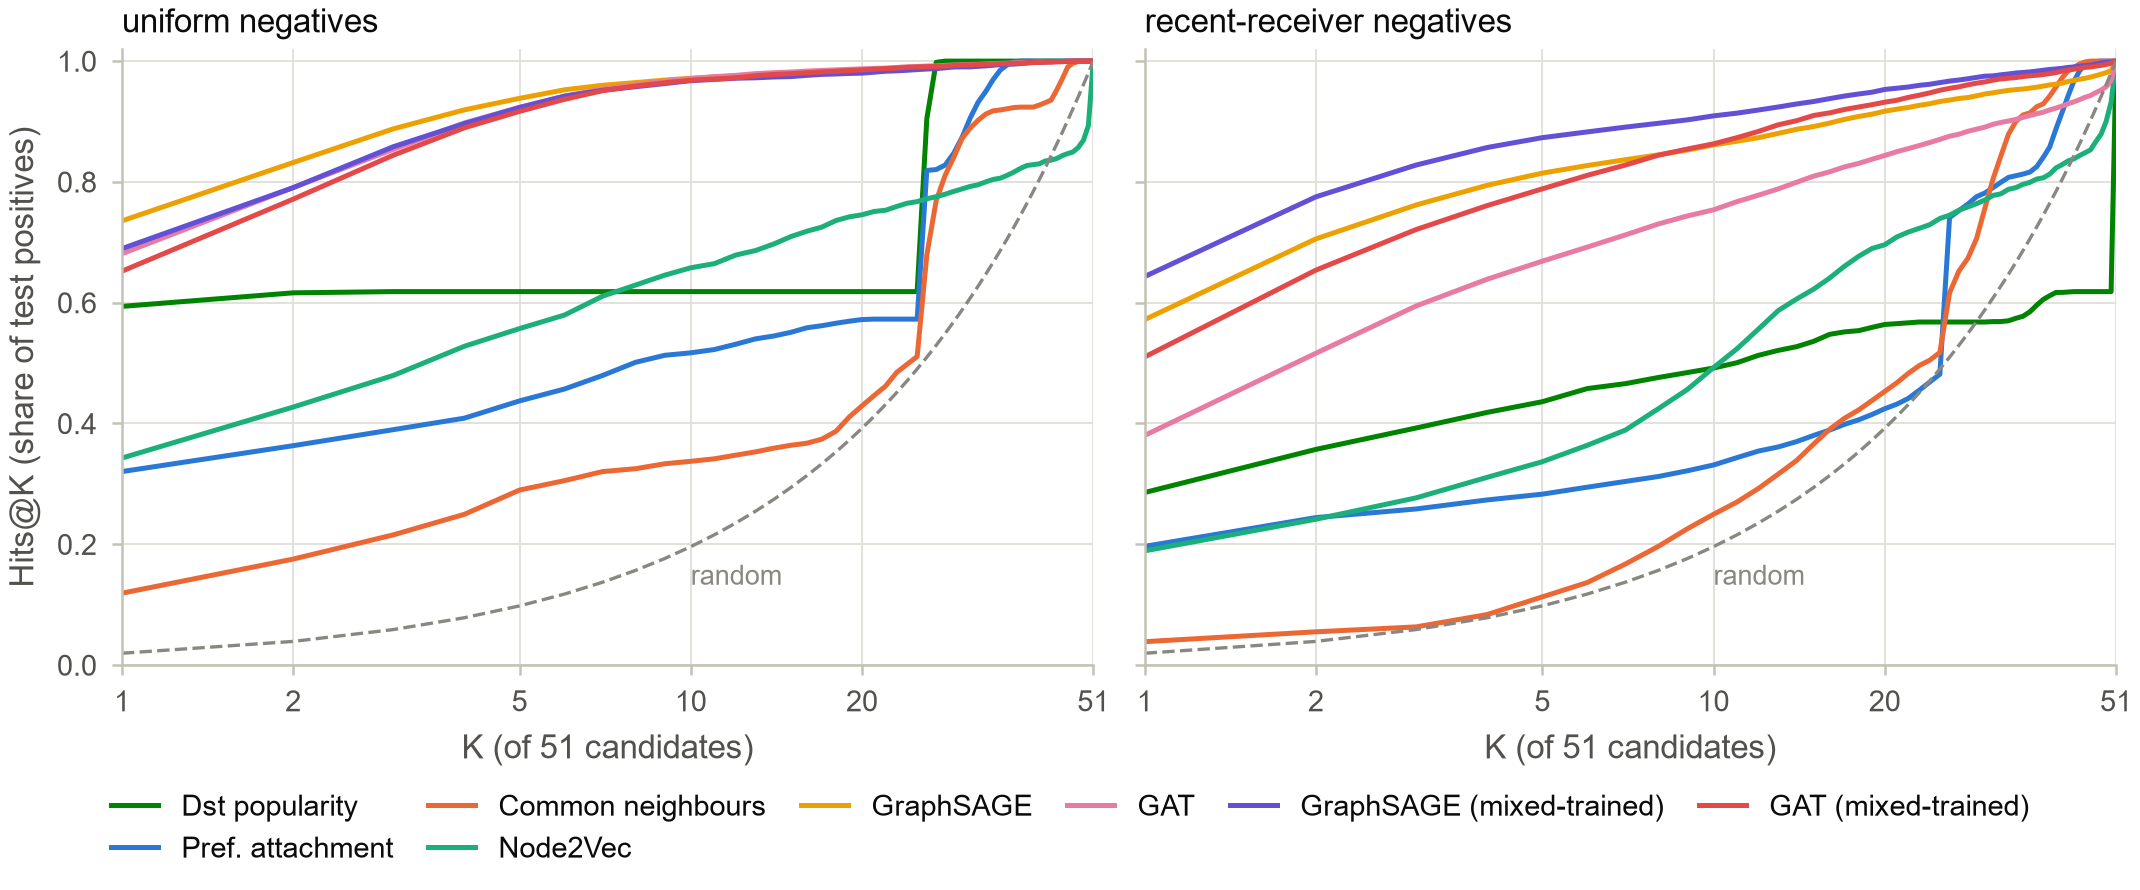
\includegraphics[width=\linewidth]{../../reports/study_B/runs/COMPLETO_2_all/figures/fig7_hits_at_k}
    \caption{Hits@K sul test per ogni $K$ da 1 a 51: quota di positivi
    ordinati entro le prime $K$ posizioni tra 51 candidati (il positivo e i
    suoi 50 negativi). Per GraphSAGE e GAT, anche con negativi misti, sono
    riuniti i tre seed. In caso
    di parità il positivo riceve il rango medio. Linea tratteggiata:
    ordinamento casuale ($K/51$).}
    \label{fig:fig7_hits_at_k}
\end{figure}

La curva mostra l'intera distribuzione del rango del positivo, di cui MRR
e Hits@10 sono riassunti. Con negativi \textbf{uniformi GraphSAGE} mette il \textbf{vero}
destinatario al \textbf{primo} posto nel \textbf{78\% dei casi} e\textbf{ GAT} nel\textbf{ 71\%}. La
curva di Dst popularity è piatta a $0{,}62$ fino a $K \approx 26$ e poi
salta a 1: è lo stesso 38\% di positivi a punteggio zero, che pareggiano con
tutti i negativi e ricevono il rango medio 26. Lo stesso salto, più
contenuto, compare per preferential attachment e common neighbours.\\ Con
negativi recenti GraphSAGE resta nettamente sopra i modelli addestrati con
negativi uniformi a ogni $K$ (Hits@1 $0{,}50$, Hits@10 $0{,}81$), ed è
superato solo da GraphSAGE con negativi misti (Hits@1 $0{,}64$, Hits@10
$0{,}91$); GAT misto arriva a Hits@1 $0{,}51$. GAT (con negativi uniformi) e Dst popularity partono da
circa $0{,}25$--$0{,}29$ a $K = 1$, Node2Vec da $0{,}19$, e common neighbours coincide
con il caso per $K < 10$.

Il \textbf{risultato dipende} anche dal \textbf{grado} della \textbf{sorgente}. Per le \textbf{sorgenti} con
\textbf{grado uscente} nella storia \textbf{inferiore a 5}, che coprono il 52\% dei positivi
di test, Dst popularity è già quasi perfetta con negativi uniformi (AP
$0{,}92$--$0{,}93$): questi indirizzi \textbf{inviano} soprattutto ai \textbf{destinatari
più popolari}, \textbf{coerentemente }con la struttura a \textbf{stella} dello Studio A. Le
sorgenti con almeno 100 controparti (39\% dei positivi) sono il caso
difficile: Dst popularity scende ad AP $0{,}08$, GraphSAGE a $0{,}42$. Con
negativi recenti l'AP dei modelli addestrati con negativi uniformi è vicina
a zero per queste sorgenti, ma GraphSAGE mantiene MRR $0{,}51$ contro
$0{,}04$ della baseline. L'AP bassa nasce dal confronto tra coppie di
sorgenti diverse, la MRR dal confronto con i negativi della stessa
sorgente. \textbf{GraphSAGE ordina} quindi \textbf{bene} i \textbf{destinatari} di un \textbf{hub}, ma con
punteggi non confrontabili con quelli delle sorgenti periferiche. Gli hub
inviano soprattutto a indirizzi \textbf{non attivi di recente} (487 dei loro 574
positivi): per questo i negativi recenti, tutti attivi, li penalizzano più
delle altre sorgenti.

\subsection{Addestramento con negativi difficili}\label{sec:negativi_misti}
I modelli precedenti vedono in addestramento solo negativi uniformi, cioè
quasi sempre indirizzi dormienti, e imparano quindi soprattutto che un
destinatario attivo è probabile. Addestrare invece \textbf{solo} con negativi
recenti produce la \textbf{scorciatoia opposta}: tutti i negativi sono attivi di
recente, mentre il 38\% dei veri destinatari di test (561 su 1\,470) non è
nel pool recente, quindi \emph{non attivo di recente} diventa sinonimo di
positivo. In un esperimento preliminare GraphSAGE addestrato così raggiunge
AP $0{,}78$ con negativi recenti, ma $0{,}999$ sui positivi fuori dal pool
e $0{,}01$ con negativi uniformi. Per questo i negativi di
addestramento sono stati \textbf{mescolati}: ciascuno viene dal pool uniforme
o da quello recente con probabilità $1/2$, così né l'attività né
l'inattività del destinatario bastano da sole a separare le classi.

La Tabella~\ref{tab:negativi_misti} divide inoltre i positivi di test in
base al fatto che il vero destinatario sia nel pool recente. Il gruppo
\emph{destinatario recente} è il confronto alla pari con i negativi
recenti: positivo e negativi sono tutti attivi, e conta solo \emph{verso
chi} invia la sorgente.

\begin{table}[H]
\centering
\caption{AP e MRR di test (media su 3 seed) per tipo di addestramento. Le
ultime due colonne usano i negativi recenti e dividono i positivi in base
al fatto che il vero destinatario sia nel pool recente (909) o no (561).}
\label{tab:negativi_misti}
\begin{tabular}{lcccc}
\toprule
Modello & Uniformi & Recenti & Dest.\ recente & Dest.\ non recente \\
\midrule
Dst popularity       & $0{,}59$ · $0{,}62$ & $0{,}15$ · $0{,}37$ & $0{,}33$ · $0{,}58$ & $0{,}02$ · $0{,}02$ \\
GraphSAGE            & $0{,}83$ · $0{,}86$ & $0{,}28$ · $0{,}62$ & $0{,}43$ · $0{,}70$ & $0{,}04$ · $0{,}49$ \\
GraphSAGE (misti)    & $0{,}70$ · $0{,}79$ & $0{,}46$ · $0{,}75$ & $0{,}47$ · $0{,}71$ & $0{,}61$ · $0{,}81$ \\
GAT                  & $0{,}74$ · $0{,}80$ & $0{,}14$ · $0{,}39$ & $0{,}23$ · $0{,}54$ & $0{,}02$ · $0{,}14$ \\
GAT (misti)          & $0{,}58$ · $0{,}76$ & $0{,}36$ · $0{,}64$ & $0{,}37$ · $0{,}65$ & $0{,}39$ · $0{,}62$ \\
\bottomrule
\end{tabular}
\end{table}

Con negativi misti GraphSAGE perde $0{,}13$ di AP sui negativi uniformi e
ne guadagna $0{,}17$ su quelli recenti, restando sopra Dst popularity in
entrambi i casi. A parità di condizioni (destinatario recente) il guadagno
è però piccolo: AP da $0{,}43$ a $0{,}47$, MRR da $0{,}70$ a $0{,}71$. La
parte maggiore del miglioramento viene dai destinatari non recenti (AP da
$0{,}04$ a $0{,}61$): il modello non premia più l'attività in sé e mette un
destinatario dormiente legato alla sorgente sopra un indirizzo attivo ma
estraneo. Questo gruppo favorisce però qualunque modello che pesi meno
l'attività, per cui il confronto di riferimento resta quello alla pari.
Lo stesso vale per gli hub: con negativi recenti l'AP di GraphSAGE sulle
sorgenti con almeno 100 controparti sale da $0{,}04$ a $0{,}68$, ma il
guadagno viene tutto dai loro destinatari non recenti (AP da $0{,}41$ a
$0{,}78$), mentre sugli 87 positivi con destinatario recente resta
invariato ($0{,}07$ contro $0{,}06$). GAT
segue lo stesso andamento con guadagni maggiori (AP alla pari da $0{,}23$ a
$0{,}37$) ma resta sotto GraphSAGE ed è molto variabile tra i seed (AP
recenti $0{,}36 \pm 0{,}10$).

\subsection{Risultati}
I risultati sono \textbf{buoni}. \textbf{GraphSAGE} è il modello migliore: con negativi
uniformi prevede bene il destinatario del prossimo trasferimento (AP $0{,}83$,
MRR $0{,}86$) e supera nettamente sia le euristiche strutturali (preferential
attachment e common neighbours, AP $< 0{,}05$) sia la baseline Dst popularity
(AP $0{,}59$). Il quadro cambia con i \textbf{negativi difficili}, cioè indirizzi
che hanno ricevuto di recente e sono quindi plausibili quanto quello vero:
l'AP di GraphSAGE scende a $0{,}28$ (MRR $0{,}62$), comunque circa il doppio
della baseline ($0{,}15$). Il motivo è l'\textbf{alto ricambio degli indirizzi}:
nel test il 39\% delle nuove coppie coinvolge indirizzi mai visti, e solo
il 62\% dei destinatari reali era attivo di recente. Addestrare con \textbf{negativi misti} porta GraphSAGE ad AP $0{,}46$
sui negativi recenti, al prezzo di $0{,}13$ di AP su quelli uniformi, ma a
parità di condizioni il guadagno è solo da $0{,}43$ a $0{,}47$. Il modello
impara quindi bene \textbf{chi} è attivo, mentre capire \textbf{verso chi} invia una data
sorgente resta difficile, soprattutto quando la sorgente è molto attiva:
per gli hub che inviano a destinatari attivi l'AP con negativi recenti
resta sotto $0{,}07$ con entrambi gli addestramenti. GAT non migliora
GraphSAGE ed è meno stabile tra i seed.


\newpage
\section{Node classification su BITCOIN}\label{sec:studioC}

Anche in questa task l'obiettivo è capire:\emph{ quanto aggiunge il grafo
rispetto all'informazione già contenuta nelle feature, e quanto di questo
vantaggio regge al cambiamento della distribuzione nel tempo}. Le figure
descrivono, nell'ordine, come cambia la popolazione da classificare, quanto
ottiene ciascun modello e quanto è affidabile la selezione dei modelli.

Ogni modello assegna a una transazione un punteggio di illeceità. Sono
confrontati due insiemi di feature: le 93 feature \emph{locali} della
transazione (l'indice del time step è escluso) e l'insieme \emph{completo}
di 165, che aggiunge le 72 feature aggregate sui vicini a un passo. Attraverso i seguenti modelli: Random
Forest (500 alberi, pesi di classe bilanciati) e MLP vedono solo le
feature. GraphSAGE e GAT (3 strati) aggregano anche le rappresentazioni dei
vicini nel grafo reso non diretto. Ogni fase usa solo il grafo visibile fino
al suo ultimo time step, comprese le transazioni etichettate come \emph{unknown}, che fanno da
contesto ma non entrano nella loss né nelle metriche. MLP e GNN sono
addestrati full-batch con una \emph{binary cross entropy} pesata per classe e
con early stopping sulla PR-AUC di validazione,
ripetuti con 5 seed; il Random Forest usa un solo seed.\\ Le metriche
riguardano la classe illecita: la \emph{PR-AUC} è l'area sotto la curva
precision--recall e non dipende da una soglia; l'\emph{F1} usa la soglia
che la massimizza in validazione, applicata invariata al test.

\begin{figure}[H]
    \centering
    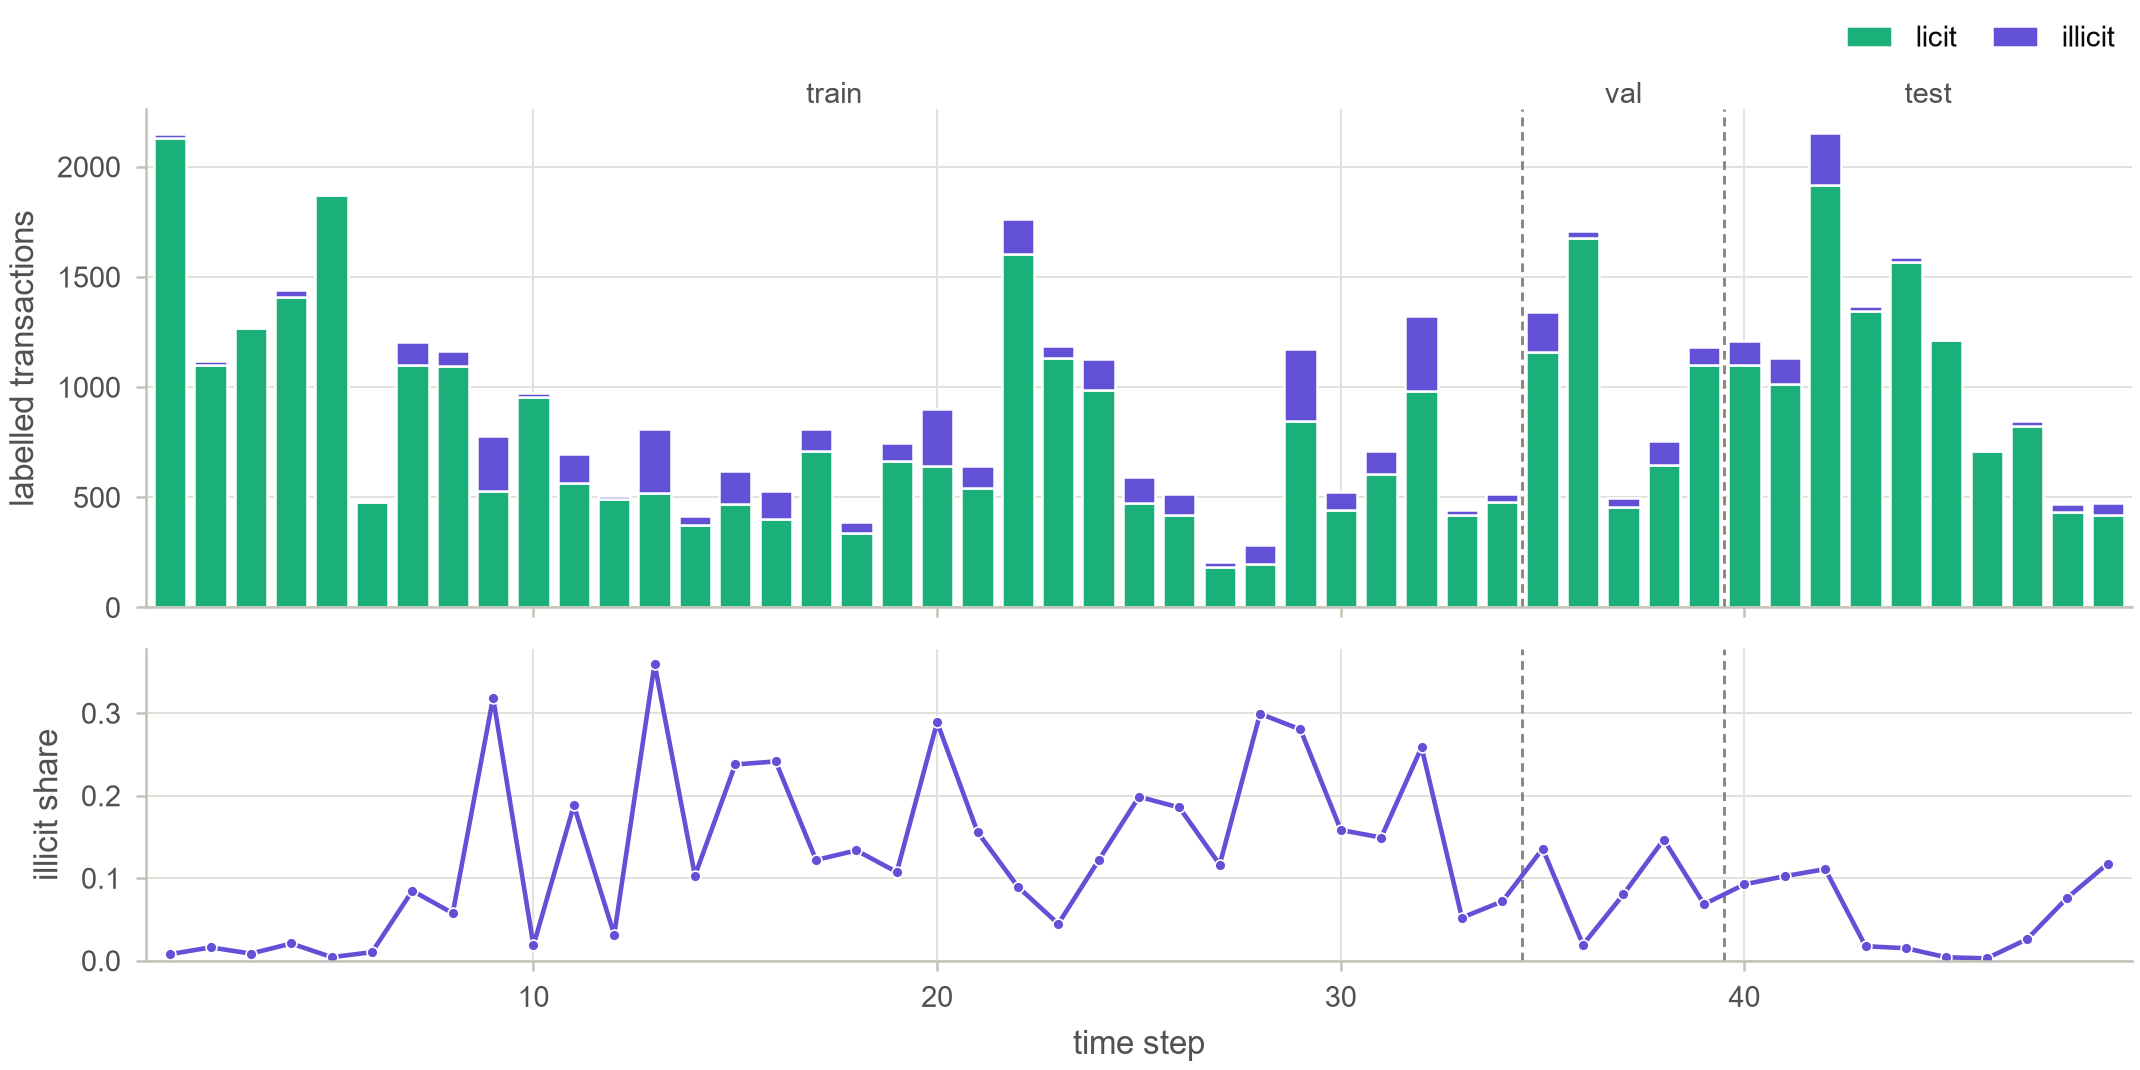
\includegraphics[width=\linewidth]{../../reports/study_C/runs/COMPLETO/figures/fig01_labels_by_step}
    \caption{Transazioni etichettate per time step (sconosciute
    omesse). Sopra: lecite e illecite. Sotto: quota illecita tra le
    etichettate. Le linee tratteggiate separano addestramento (1--34),
    validazione (35--39) e test (40--49).}
    \label{fig:fig01_labels_by_step}
\end{figure}

La quota illecita varia molto da un time step all'altro: è quasi nulla nei
primi sei, supera il 30\% in alcuni step dell'addestramento e scende in
media dall'11,6\% dell'addestramento al 5,7\% del test
(Tabella~\ref{tab:elliptic_split}). Il \textbf{test} è inoltre molto \textbf{disomogeneo}.
Gli step 40--42 contengono 467 delle 636 transazioni illecite (73\%),
mentre dal 43 al 46 se ne contano al più 24, in corrispondenza
dell'evento esterno descritto da Weber et al.\ \cite{weber2019elliptic}, chiusura di un dark market. Le
metriche di test misurano quindi soprattutto la capacità di riconoscere le
illecite dei primi tre step di test, e un modello addestrato su una
distribuzione deve essere valutato su un'altra.

\begin{figure}[H]
    \centering
    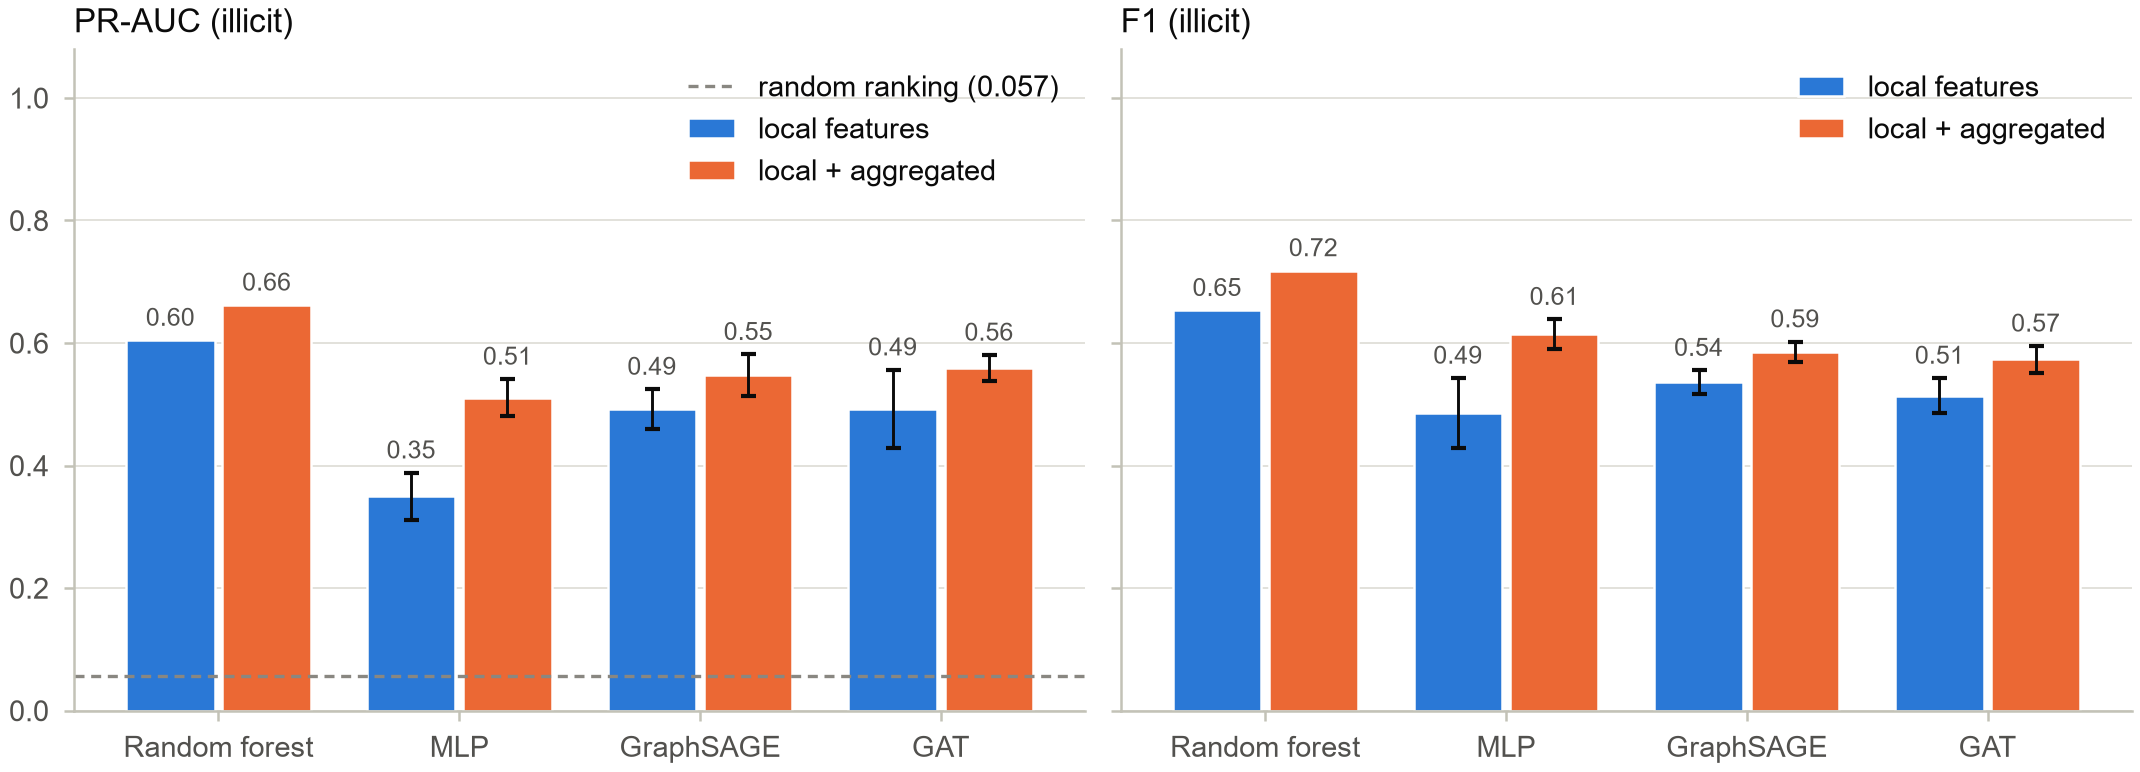
\includegraphics[width=\linewidth]{../../reports/study_C/runs/COMPLETO/figures/fig02_test_metrics}
    \caption{PR-AUC e F1 della classe illecita sul test, per modello e
    insieme di feature. Per MLP, GraphSAGE e GAT media $\pm$ deviazione
    standard. Linea
    tratteggiata: PR-AUC di un ordinamento casuale (prevalenza, $0{,}057$).}
    \label{fig:fig02_test_metrics}
\end{figure}

Il \textbf{Random Forest} è il modello \textbf{migliore} con entrambi gli insiemi di feature
(PR-AUC $0{,}60$ e $0{,}66$, F1 $0{,}65$ e $0{,}72$).
Le feature aggregate migliorano tutti i modelli, quindi \textbf{l'informazione di
vicinato è utile}. Con le sole feature locali le GNN superano nettamente
l'MLP, che ha la stessa architettura senza grafo (PR-AUC $0{,}49$ contro
$0{,}35$): qui il \textbf{grafo fornisce informazione} che le feature non hanno. Con
l'insieme completo il vantaggio si riduce a $0{,}04$--$0{,}05$ di PR-AUC,
dell'ordine di 1--2 deviazioni standard, e per l'F1 si inverte (MLP $0{,}61$,
GraphSAGE $0{,}59$, GAT $0{,}57$). Le \textbf{feature aggregate catturano} quindi gran
parte di \textbf{ciò che le GNN ricavano} dal vicinato, e nessuna GNN raggiunge il
Random Forest. Tutti i modelli hanno precisione alta (da $0{,}74$ a $0{,}97$
con l'insieme completo) e recall bassa (da $0{,}44$ a $0{,}57$). Le illecite
mancate sono soprattutto quelle successive allo step 42: dallo step 43 l'F1
per step scende quasi a zero per tutti i modelli, con la sola eccezione
dello step 46, che contiene 2 illecite.\\

Il motivo per cui il \textbf{grafo} è \textbf{utile} emerge dall'\textbf{omofilia delle etichette}
lungo gli archi. In addestramento il \textbf{vicino di
una transazione illecita} è \textbf{illecito} nel \textbf{58\% dei casi}, contro il \textbf{6\%}
atteso\textbf{ senza omofilia}, mentre quello di una lecita lo è solo nel 3\%;
l'\textbf{assortatività} delle etichette \cite{newman2002assortative} è \textbf{$r =
0{,}55$}. Il segnale resta forte nel test ($0{,}46$, $r = 0{,}45$) ma si
dimezza in validazione ($0{,}30$, $r = 0{,}27$).\emph{ L'omofilia giustifica
l'uso del vicinato.}
Riguarda però \textbf{vicini a un passo}, già \textbf{riassunti} dalle
\textbf{feature aggregate}, e questo \textbf{spiega} perché il \textbf{guadagno} delle \textbf{GNN} sia ampio
solo con le feature \textbf{locali}. Inoltre la validazione, su cui si scelgono
epoca e soglia, ha una struttura di vicinato meno informativa del test, e
quindi seleziona i modelli su un segnale diverso da quello su cui vengono
valutati.

\begin{figure}[H]
    \centering
    % riga più larga del testo (1,25 \textwidth), centrata e sporgente su entrambi i margini
    \makebox[\textwidth][c]{\begin{minipage}{1.25\textwidth}
    \begin{subfigure}[b]{0.32\linewidth}
        \centering
        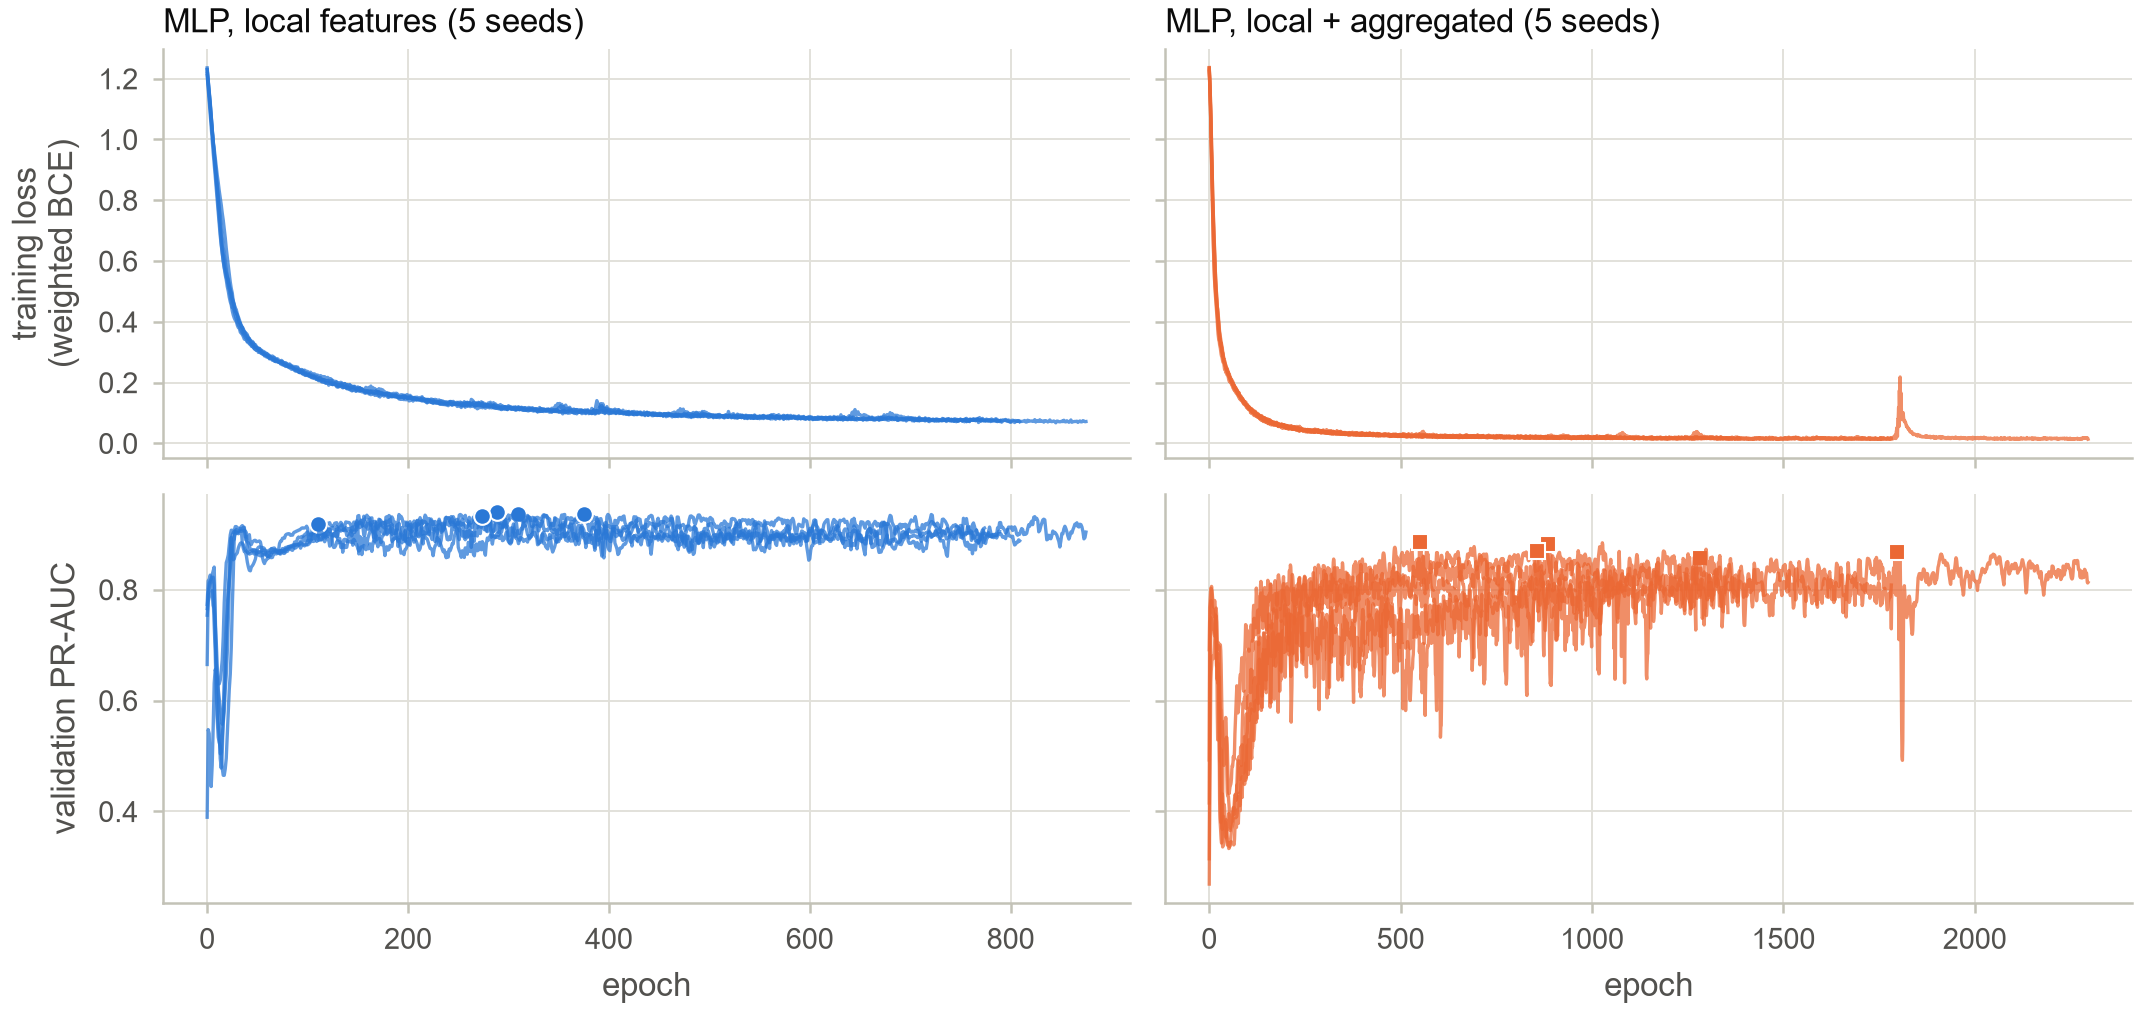
\includegraphics[width=\linewidth]{../../reports/study_C/runs/COMPLETO/figures/fig05_learning_mlp}
        \caption{MLP}
        \label{fig:fig05_learning_mlp}
    \end{subfigure}\hfill
    \begin{subfigure}[b]{0.32\linewidth}
        \centering
        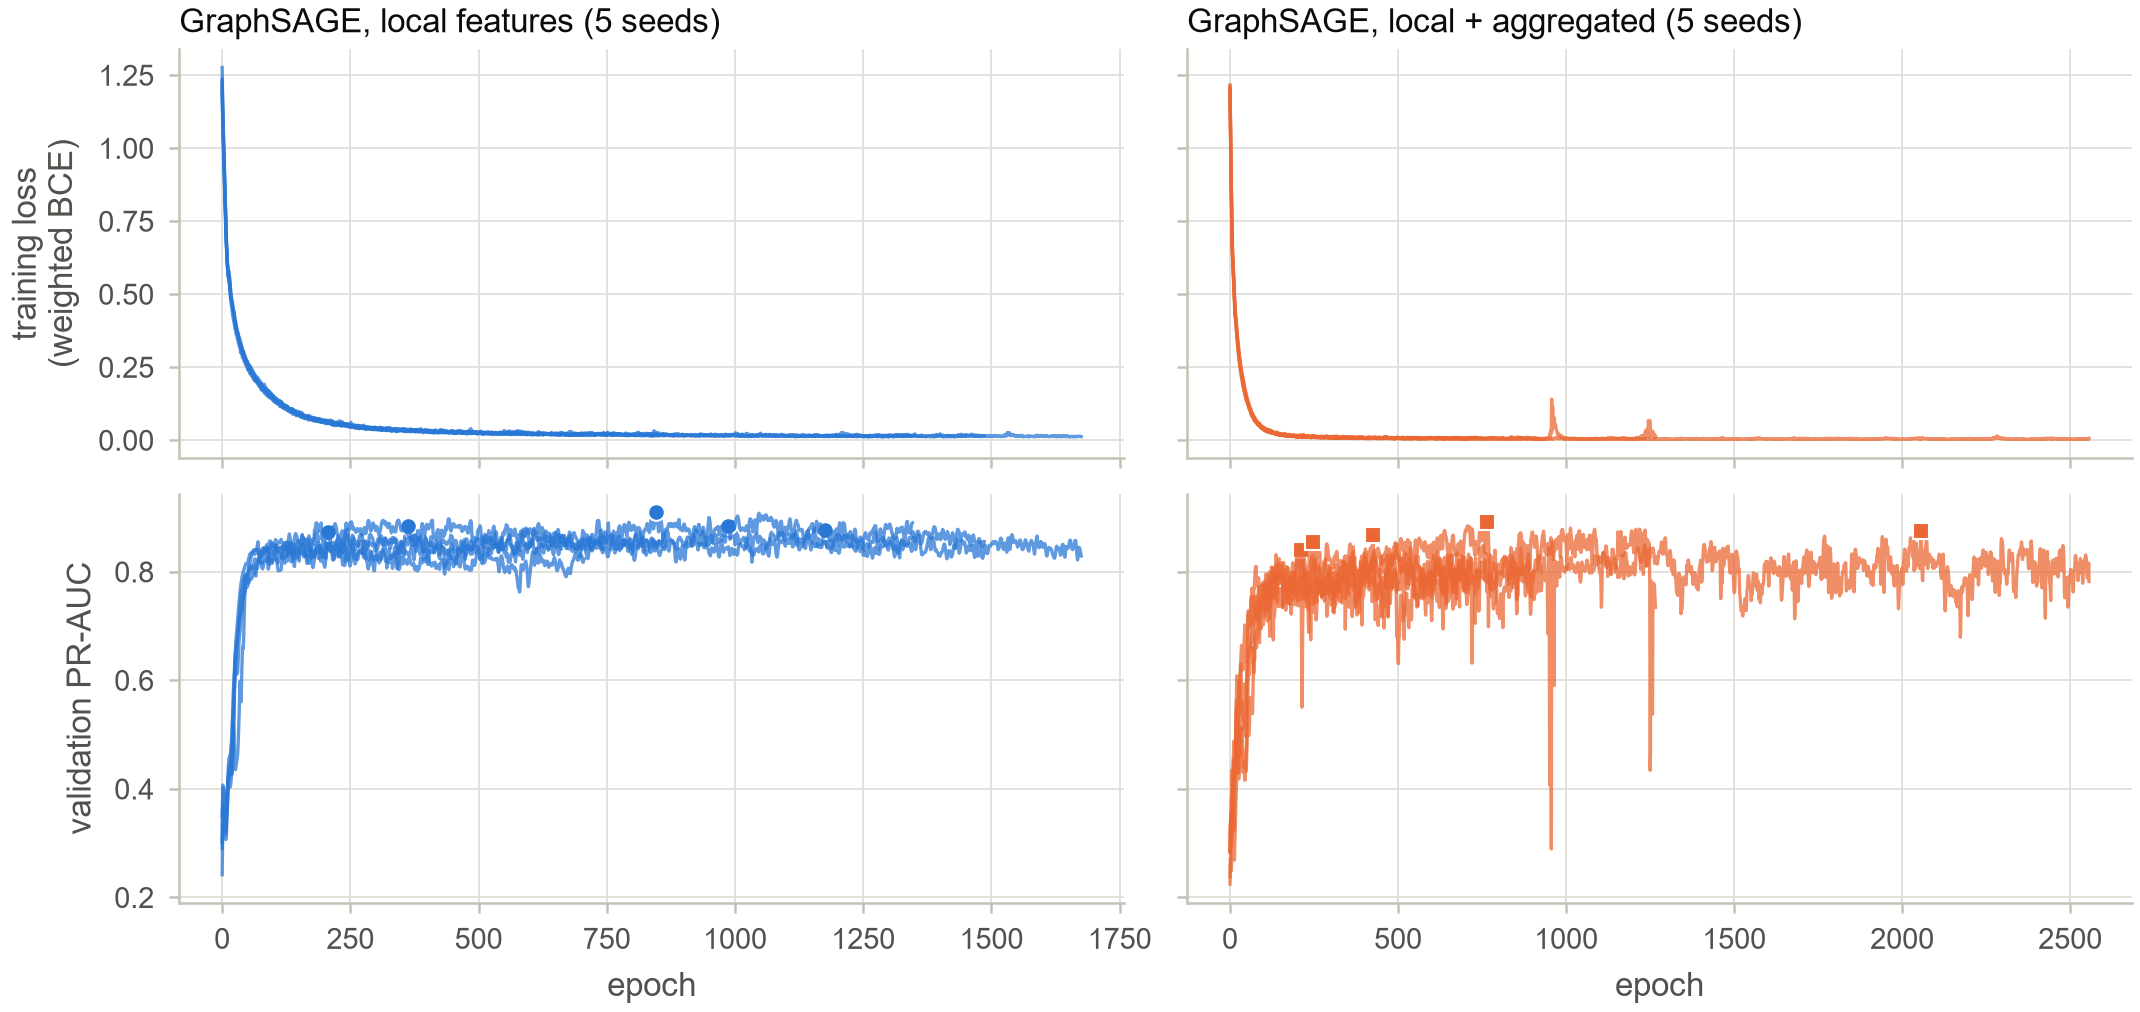
\includegraphics[width=\linewidth]{../../reports/study_C/runs/COMPLETO/figures/fig05_learning_graphsage}
        \caption{GraphSAGE}
        \label{fig:fig05_learning_graphsage}
    \end{subfigure}\hfill
    \begin{subfigure}[b]{0.32\linewidth}
        \centering
        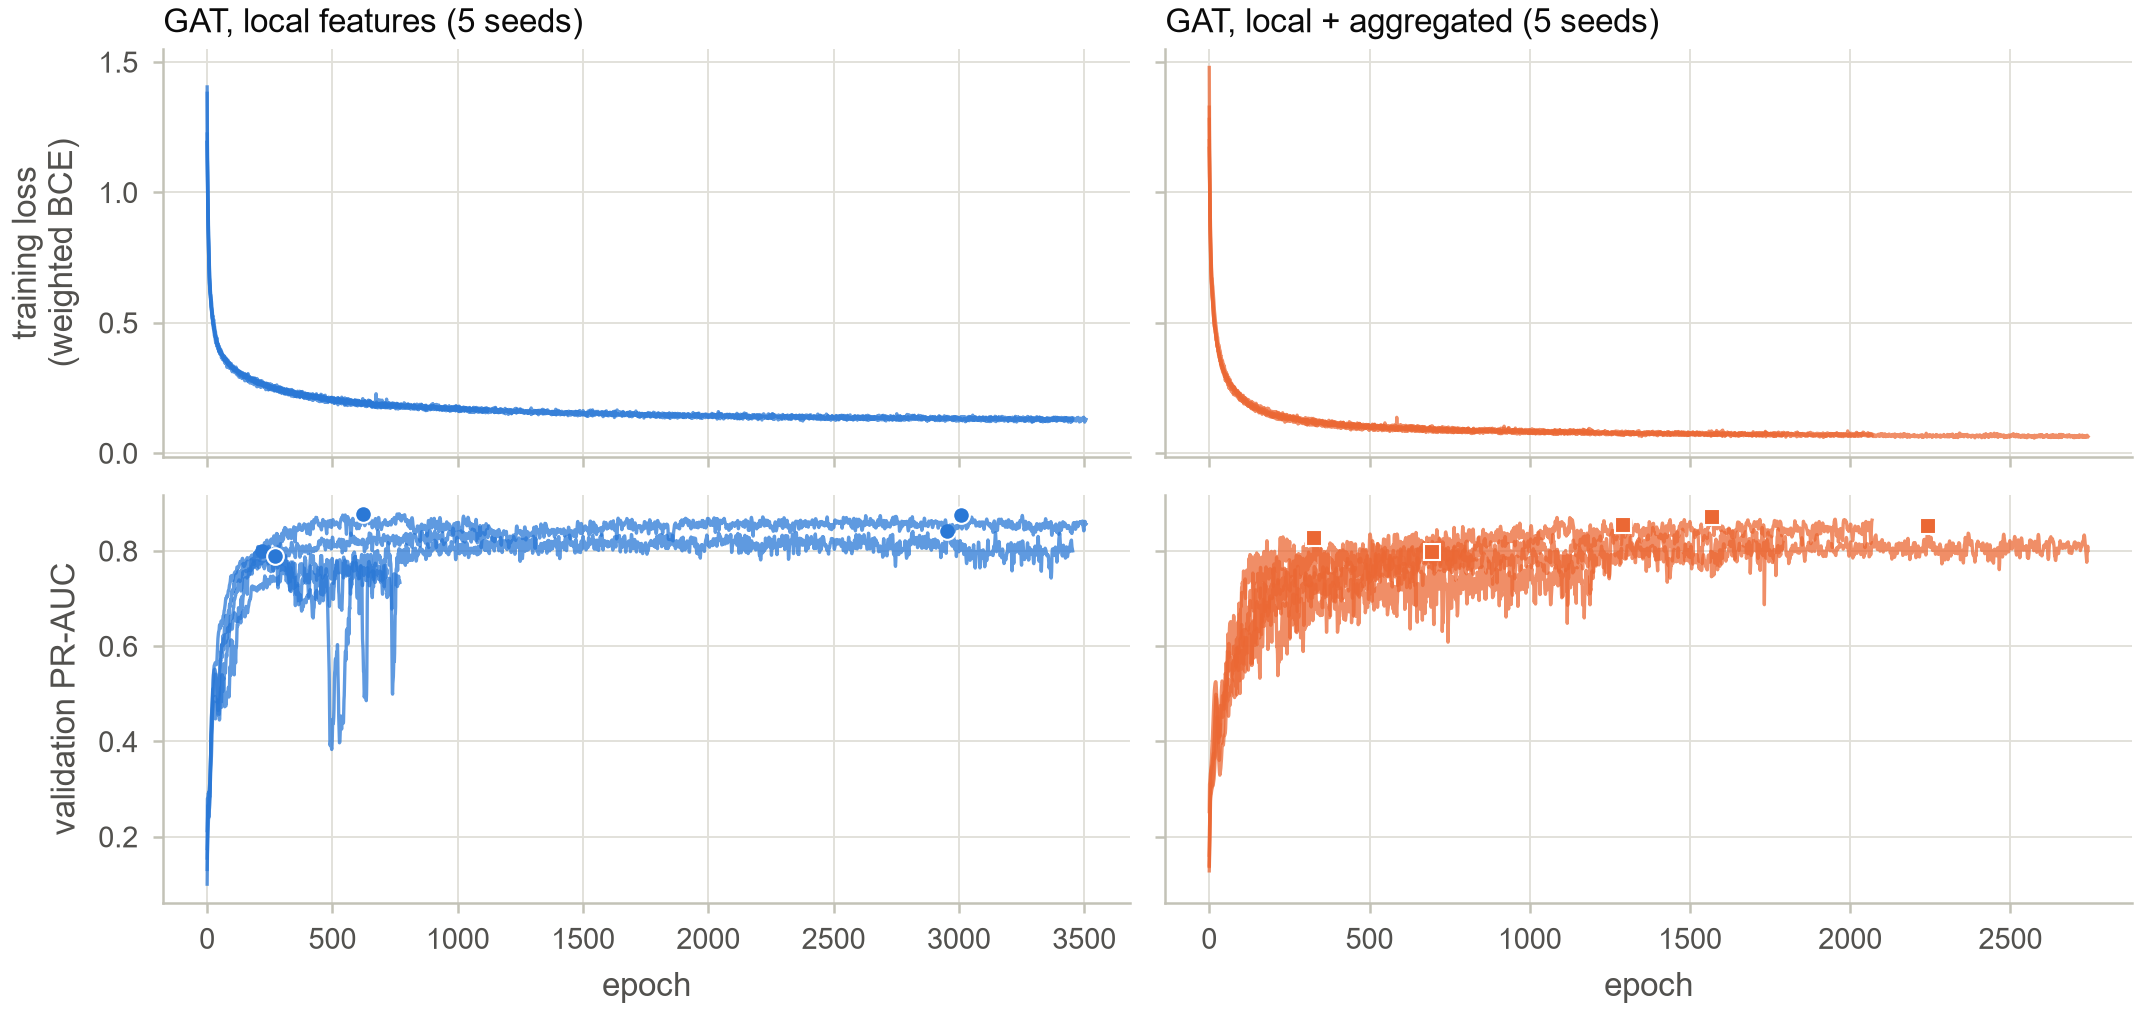
\includegraphics[width=\linewidth]{../../reports/study_C/runs/COMPLETO/figures/fig05_learning_gat}
        \caption{GAT}
        \label{fig:fig05_learning_gat}
    \end{subfigure}
    \end{minipage}}
    \caption{Curve di apprendimento, una linea per seed; in ogni pannello
    feature locali a sinistra e insieme completo a destra. Sopra: loss di
    addestramento (cross entropy pesata). Sotto: PR-AUC di
    validazione; il marcatore indica l'epoca selezionata, i cui pesi sono
    conservati.}
    \label{fig:fig05_learning}
\end{figure}

In tutti i modelli la loss di addestramento continua a scendere (fino a
$0{,}01$--$0{,}13$), mentre la PR-AUC di validazione raggiunge un plateau tra
$0{,}8$ e $0{,}9$ già nelle prime 100--300 epoche: le epoche successive migliorano solo l'adattamento
ai dati di addestramento. Con l'insieme completo le curve di validazione
oscillano molto di più, e le epoche selezionate sono sparse lungo il
plateau (MLP da 550 a $1\,796$, GraphSAGE da 211 a $2\,056$, GAT da 328 a
$2\,242$): la scelta dell'epoca dipende in buona parte dal rumore. Per GAT
con feature locali due seed si fermano presto (circa 750 epoche) su valori
più bassi ($0{,}79$--$0{,}80$) degli altri tre ($0{,}84$--$0{,}88$), da cui
la sua deviazione standard più ampia sul test. Infine, la PR-AUC di
validazione non predice quella di test. L'MLP con feature locali ha la
validazione migliore tra i modelli neurali ($0{,}93$) e il test peggiore ($0{,}35$),
mentre le GNN hanno validazioni più basse ma test migliori. Il cambiamento
di distribuzione tra le fasi pesa più delle differenze tra modelli
osservate in validazione.



\section{Discussione e limiti}\label{sec:discussione}

I tre studi danno una risposta coerente: la \textbf{struttura} del \textbf{grafo} contiene
\textbf{informazione utile}, ma il suo \textbf{valore aggiunto dipende} da quanto di essa è
\textbf{già disponibile} in forma più semplice.

Lo Studio A mostra reti organizzate
attorno a pochi hub, con volume estremamente concentrato (Gini maggiore di
$0{,}95$), periferia a stella priva di triangoli e alto ricambio mensile.

\begin{quote}
\fbox{\parbox{\dimexpr\linewidth-2\fboxsep-2\fboxrule}{\itshape
Le reti mostrano \textbf{gradi eterogenei a coda pesante} e \textbf{distanze
medie brevi}, tipiche di molte reti reali, ma \textbf{non sono né scale-free}
(la power-law è rifiutata nella maggior parte dei casi) \textbf{né
small-world} (clustering inferiore al modello nullo, $\sigma < 1$). La
struttura è più vicina a un modello \textbf{hub-and-spoke disassortativo}.}}
\end{quote}

Questa struttura spiega i risultati dello Studio B. Sapere \emph{chi} è attivo
basta già a una baseline di sola popolarità per ottenere buona parte delle
prestazioni con negativi uniformi, mentre le euristiche basate su vicini
comuni falliscono per l'assenza di triangoli. Solo GraphSAGE estrae
informazione aggiuntiva su \emph{a chi} una sorgente invierà, ed è
l'unico modello addestrato con negativi uniformi il cui vantaggio regge
ai negativi recenti in tutte le settimane di test; con negativi misti ci
riesce anche GAT, ma il guadagno a parità di attività del destinatario
resta piccolo.

Nello Studio C l'omofilia delle etichette rende il vicinato
informativo, e le GNN superano nettamente l'MLP quando dispongono delle sole
feature locali. Quando le feature aggregate riassumono già il vicinato a un
passo, però, il guadagno si riduce, e il
Random Forest resta il modello migliore. Il \textbf{grafo aggiunge} quindi
\textbf{informazione quando }questa \textbf{non è già codificata nelle feature} o nella
popolarità dei nodi, non in generale.

\paragraph{Validità temporale.}
Nessuna delle reti analizzate è stazionaria. L'attività dei token ERC-20 cala
di circa due ordini di grandezza, e nello Studio B i modelli sono
addestrati su settimane con decine di volte più positivi del test. In
Elliptic la quota illecita scende dall'$11{,}6\%$ al $5{,}7\%$, e dallo
step 43 tutti i modelli perdono quasi del tutto la capacità di riconoscere le
illecite. Anche la selezione dei modelli ne risente: nello Studio C, tra i modelli
neurali, l'ordinamento in validazione non corrisponde a quello in test
(l'MLP con feature locali è il migliore in validazione e il peggiore in
test). Le prestazioni riportate valgono per i periodi
osservati e non vanno estese ad altri periodi senza una nuova validazione.

\paragraph{Semantica dei dati e identità.}
Un indirizzo non corrisponde a una persona o a un'organizzazione: un'entità
può controllare molti indirizzi e un indirizzo, come un contratto, può
servire molti utenti. \textbf{Hub, community e indirizzi condivisi tra token sono
quindi descrittori strutturali e non trader, exchange o contratti del mondo reale.}
A meno di un controllo 1:1 attraverlo la ricerca online degli indirizzi per capire se si hanno degli intendificativi. Come l'unica
attribuzione presente, quella del router di MetaMask, che si basa su un'etichetta
pubblica di Etherscan verificata in modo indipendente. Gli importi sono
in unità on-chain grezze e non sono confrontabili tra token. I trasferimenti
unici sono ricostruiti da snapshot sovrapposti; la ricostruzione è coerente
su tutti i token, ma trasferimenti identici nello stesso giorno sono
distinguibili solo tramite la loro molteplicità. Le etichette di Elliptic
coprono solo il $22{,}9\%$ delle transazioni e derivano da una
classificazione delle entità che non è pubblica: i risultati sono una
valutazione su un benchmark e non una capacità di rilevare frodi reali.

\paragraph{Scelte metodologiche e approssimazioni.}
Diverse misure dello Studio A usano la proiezione non diretta (clustering,
cammini, assortatività, community), che ignora il verso dei flussi; per
grafi grandi betweenness, closeness armonica e cammini medi sono stimati da
un campione di sorgenti, e il confronto small-world si basa su 15 grafi
nulli per mese. Nello Studio B le coppie con un indirizzo mai visto (il 39\%
dei nuovi legami nel test) sono escluse, quindi i risultati valgono solo per
indirizzi già attivi. I negativi sono campionati (50 per positivo).
L'addestramento con negativi misti usa una sola proporzione ($1/2$), non
ottimizzata, e i negativi di addestramento possono includere raramente
coppie che diventeranno vere (falsi negativi), più probabili nel pool
recente perché è piccolo (in media 365 indirizzi nelle settimane di test). Gli iperparametri delle GNN non
sono stati ottimizzati in modo sistematico, le GNN sono ripetute con 3 seed
(Studio B) e 5 seed (Studio C), e il Random Forest con un solo seed, per cui
la sua variabilità non è stimata. Per Node2Vec la libreria usata
(torch-cluster 1.6.3) campiona correttamente le walk biased solo per
$q \ge 1$ e $p \le q$, quindi il regime $q < 1$ (walk che si allontanano
dal nodo di partenza) non è stato esplorato.

\paragraph{Generalizzabilità.}
Lo Studio A copre 4 degli 84 token di TGS, scelti per numero di
trasferimenti, e BITCOIN copre solo cinque mesi; lo Studio B usa un solo
token. I token più piccoli potrebbero avere strutture diverse. Elliptic
descrive un unico periodo di Bitcoin con feature anonimizzate, e il
\textbf{vantaggio} delle\textbf{ feature aggregate potrebbe non trasferirsi }a \textbf{dataset} in cui
il \textbf{vicinato non} è già \textbf{riassunto}.


\paragraph{Sviluppi futuri.}
Le estensioni più dirette sono: modelli temporali che usino la sequenza
degli eventi invece di snapshot cumulativi; un protocollo induttivo per gli indirizzi
senza storia; la calibrazione dei punteggi tra sorgenti diverse, che oggi
penalizza gli hub nell'AP; la ripetizione su più token e la ricalibrazione
periodica della soglia di classificazione in Elliptic.

\newpage
\section{Conclusioni}\label{sec:conclusioni}

Questo lavoro ha studiato se la rappresentazione a grafo di dati blockchain
fornisca informazione utile oltre alle tecniche standard, con tre studi
valutati sempre in ordine temporale.

Le reti di trasferimento dei token ERC-20 analizzate sono dominate da pochi
indirizzi centrali, che concentrano attività e volume, attorno ai quali
ruota una periferia ampia, poco connessa e in continuo ricambio. Le
distribuzioni hanno code pesanti, ma i test non supportano la legge di
potenza né l'ipotesi small-world. Le community esistono ma sono fortemente
collegate tra loro, e gli indirizzi attivi su più token sono una minoranza
strutturalmente centrale.

Nella previsione di nuovi legami sul token SWAP, gran parte del successo
apparente con negativi uniformi deriva dal riconoscere gli indirizzi attivi.
Con negativi recenti solo GraphSAGE supera in modo stabile una baseline di
sola popolarità (AP $0{,}28$ contro $0{,}15$, MRR $0{,}62$ contro $0{,}37$).
Addestrare con negativi misti porta l'AP a $0{,}46$, ma a parità di
attività del destinatario il guadagno è solo da $0{,}43$ a $0{,}47$.

Nella classificazione delle transazioni di Elliptic, il grafo è utile
quando le feature non contengono già il vicinato. Con l'insieme completo di
feature il Random Forest resta il modello migliore (PR-AUC $0{,}66$) e tutti
i modelli perdono efficacia dopo il cambiamento di distribuzione dello step
43.

Nel complesso, il valore della struttura del grafo è reale ma condizionato:
va misurato contro baseline che catturano popolarità e informazione di
vicinato già disponibili, con negativi difficili e con un protocollo
cronologico. Senza questi controlli, nei nostri esperimenti, il contributo delle GNN
risulterebbe sovrastimato.

\newpage
\bibliographystyle{plain}
\bibliography{references}

\end{document}


